\documentclass[lang=cn,newtx,10pt,scheme=chinese]{elegantbook}

\title{深入浅出数据结构}
\subtitle{北街学长倾力之作}

\author{北街}
% \institute{Elegant\LaTeX{} Program}
\date{2022/12/31}
\version{1.0}
% \bioinfo{自定义}{信息}

% \extrainfo{注意:本模板自 2023 年 1 月 122222 日开始,不再更新和维护!}

\setcounter{tocdepth}{3}

\logo{logo-blue.png}
\cover{cover.jpg}

% 本文档命令
\usepackage{array}
\newcommand{\ccr}[1]{\makecell{{\color{#1}\rule{1cm}{1cm}}}}

% 修改标题页的橙色带
\definecolor{customcolor}{RGB}{32,178,170}
\colorlet{coverlinecolor}{customcolor}
\usepackage{cprotect}

\addbibresource[location=local]{reference.bib} % 参考文献,不要删除
\usepackage{listings}         % 导入listings宏包
\usepackage{xcolor}           % 支持颜色

% 配置C++代码样式
\lstset{
    language=C++,             % 语言设置为C++
    basicstyle=\ttfamily,      % 基本样式
    keywordstyle=\color{blue}, % 关键词颜色
    commentstyle=\color{green},% 注释颜色
    stringstyle=\color{red},   % 字符串颜色
    numbers=left,              % 显示行号
    numberstyle=\tiny,         % 行号样式
    stepnumber=1,              % 每行显示行号
    breaklines=true,           % 自动换行
    frame=lines                % 代码块边框样式
}
\begin{document}

\maketitle
\frontmatter

\tableofcontents

\mainmatter

\chapter{数据结构与算法}

\section{数据结构}

\subsection{定义}
数据结构是什么?简单来说,它是用来组织和存储数据的一种方式。就像你整理房间时,衣服放衣柜,书籍放书架,零食藏在抽屉里(别骗我,你一定有零食抽屉!)。数据结构就是计算机世界里的“收纳神器”,它决定了数据的存储方式和操作效率。

\subsection{逻辑结构}
逻辑结构是数据之间的关系,就像你和朋友之间的关系一样复杂(或者简单)。根据数据元素之间的关系,逻辑结构可以分为以下几类:
\begin{itemize}
    \item \textbf{集合结构}:数据之间没有任何关系,就像一群互不认识的人站在公交车站。
    \item \textbf{线性结构}:数据之间有一对一的关系,就像排队买奶茶,每个人前后都有一个邻居。
    \item \textbf{树形结构}:数据之间有一对多的关系,就像家谱,祖宗有很多子孙。
    \item \textbf{图形结构}:数据之间有多对多的关系,就像社交网络,人人都可能是朋友(或者敌人)。
\end{itemize}

\subsection{存储结构}
存储结构是数据在计算机中的存储方式,决定了数据的“住址”。主要有以下两种:
\begin{itemize}
    \item \textbf{顺序存储}:数据存储在连续的存储单元中,就像一排整齐的书架。优点是访问速度快,缺点是插入和删除操作麻烦。
    \item \textbf{链式存储}:数据存储在不连续的存储单元中,通过指针连接,就像一串珍珠项链。优点是插入和删除方便,缺点是访问速度稍慢。
\end{itemize}
选择哪种存储方式,就像选择住公寓还是住别墅,各有利弊,关键看需求。

\section{算法}

\subsection{定义}
算法是解决问题的一组明确指令。它就像做菜的菜谱,告诉你每一步该干什么。比如,“煮方便面”这个算法可能是这样的:
\begin{enumerate}
    \item 烧水。
    \item 水开后放入面饼。
    \item 等3分钟,加入调料包。
    \item 搅拌均匀,开吃!
\end{enumerate}
一个好的算法不仅要能解决问题,还要高效,毕竟没人想等水烧开等到天荒地老。

\subsection{特征}
算法有以下几个显著特征:
\begin{itemize}
    \item \textbf{有穷性}:算法必须在有限步骤内结束,就像煮方便面不能煮一辈子。
    \item \textbf{确定性}:算法的每一步都有明确的定义,不会让你“随便加点盐”。
    \item \textbf{可行性}:算法的每一步都可以通过基本操作实现,比如“烧水”是可行的,但“召唤龙卷风”就不行。
    \item \textbf{输入}:算法可以有零个或多个输入,比如煮方便面需要水和面饼。
    \item \textbf{输出}:算法至少有一个输出,比如煮好的方便面。
\end{itemize}

\subsection{目标}
设计算法的目标是让它又快又省。具体来说:
\begin{itemize}
    \item \textbf{减少时间复杂度}:让算法运行得更快,就像希望快递能当天送达。
    \item \textbf{减少空间复杂度}:让算法占用更少的内存,就像希望行李箱能装下更多东西。
\end{itemize}
一个好的算法就像一个优秀的厨师,既能快速做好饭,又不浪费食材。

\subsection{复杂度计算}
算法复杂度是衡量算法效率的重要指标,分为时间复杂度和空间复杂度。它们是评估算法性能的核心标准,就像评估一辆车的油耗和速度,既要省油又要跑得快才是好车。

\subsubsection{时间复杂度}
时间复杂度描述算法运行所需的时间,通常用大 $O$ 表示法来表示。以下是一些常见的时间复杂度及其含义:

\begin{itemize}
    \item \textbf{$O(1)$:常数时间}
    无论输入规模多大,算法的运行时间都保持不变。
    \textit{示例}:访问数组中的某个元素,例如 $arr[5]$。
    \textit{解释}:直接定位到数组的第六个元素(索引从 0 开始),不需要额外的计算。

    \item \textbf{$O(n)$:线性时间}
    算法的运行时间与输入规模成正比。
    \textit{示例}:计算一个数组中所有元素的和。
    \textit{解释}:假设数组有 $n$ 个元素,算法需要遍历每个元素一次,因此运行时间为 $O(n)$。

    \item \textbf{$O(n^2)$:平方时间}
    算法的运行时间与输入规模的平方成正比。
    \textit{示例}:对一个数组中的所有元素两两比较,例如冒泡排序。
    \textit{解释}:对于 $n$ 个元素,每个元素需要与其他 $n-1$ 个元素进行比较,总共需要执行 $n \times (n-1)$ 次操作,近似为 $O(n^2)$。

    \item \textbf{$O(\log n)$:对数时间}
    算法的运行时间随着输入规模的对数增长。
    \textit{示例}:在一个有序数组中使用二分查找。
    \textit{解释}:每次查找都会将搜索范围缩小一半,因此运行时间为 $O(\log n)$。

    \item \textbf{$O(n \log n)$:线性对数时间}
    常见于高效的排序算法,例如归并排序和快速排序。
    \textit{示例}:对一个数组进行快速排序。
    \textit{解释}:快速排序在每次划分时需要 $O(n)$ 的时间,而划分的次数为 $O(\log n)$,因此总时间复杂度为 $O(n \log n)$。
\end{itemize}

\textbf{计算示例:}
假设我们有一个数组 $arr = [3, 1, 4, 1, 5]$,我们想要计算数组中所有元素的平方和:
\begin{verbatim}
for i in arr:
    result += i * i
\end{verbatim}
该算法需要遍历数组中的每个元素一次,因此时间复杂度为 $O(n)$。

\subsubsection{空间复杂度}
空间复杂度描述算法运行所需的存储空间,通常也用大 $O$ 表示法。以下是一些常见的空间复杂度及其含义:

\begin{itemize}
    \item \textbf{$O(1)$:常数空间}
    算法所需的额外空间不随输入规模的变化而变化。
    \textit{示例}:交换两个变量的值。
    \textit{解释}:只需要一个临时变量来存储中间值,额外空间为常数。

    \item \textbf{$O(n)$:线性空间}
    算法所需的额外空间与输入规模成正比。
    \textit{示例}:创建一个与输入数组大小相同的数组来存储结果。
    \textit{解释}:如果输入数组有 $n$ 个元素,额外需要 $n$ 个存储单元。

    \item \textbf{$O(n^2)$:平方空间}
    算法所需的额外空间与输入规模的平方成正比。
    \textit{示例}:创建一个 $n \times n$ 的二维矩阵。
    \textit{解释}:如果矩阵的维度为 $n$,则需要 $n^2$ 个存储单元。
\end{itemize}

\textbf{计算示例:}
假设我们需要存储一个二维数组的转置矩阵:
\begin{verbatim}
for i in range(n):
    for j in range(n):
        transpose[j][i] = matrix[i][j]
\end{verbatim}
如果原始矩阵的大小为 $n \times n$,则需要额外的 $n^2$ 空间来存储转置矩阵,因此空间复杂度为 $O(n^2)$。

\subsubsection{综合示例}
假设我们需要对一个数组进行排序并统计其中每个元素出现的次数:
\begin{itemize}
    \item 排序算法使用快速排序,时间复杂度为 $O(n \log n)$。
    \item 统计元素出现次数需要一个哈希表,空间复杂度为 $O(n)$。
\end{itemize}
因此,该算法的总时间复杂度为 $O(n \log n)$,空间复杂度为 $O(n)$。

通过这些示例,我们可以更直观地理解时间复杂度和空间复杂度的概念。复杂度计算就像评估一辆车的性能,既要跑得快(时间复杂度低),又要省油(空间复杂度低),才能称得上是一辆好车。

\chapter{线性表}

\section{线性表的逻辑结构}
线性表是一种最基本、最常用的数据结构,它的特点是数据元素之间存在一对一的线性关系。可以把它想象成排队买奶茶的队伍,每个人前后都有一个邻居,队伍的顺序非常重要。

线性表的逻辑结构可以用数学形式表示为:
$L = \{a_1, a_2, \dots, a_n\}$,其中 $a_i$ 表示线性表中的第 $i$ 个元素,$1 \leq i \leq n$。
\textit{示例}:假设线性表存储的是一周的日程安排:
$L = \{\text{周一}, \text{周二}, \text{周三}, \text{周四}, \text{周五}\}$。

线性表的特点:
\begin{itemize}
    \item 有且仅有一个“第一个”元素(队伍的开头)。
    \item 有且仅有一个“最后一个”元素(队伍的末尾)。
    \item 除了第一个和最后一个元素外,每个元素都有一个前驱和一个后继。
\end{itemize}

\section{顺序表}

\subsection{顺序表的定义}
顺序表是一种线性表的存储结构,它使用一组地址连续的存储单元依次存储线性表中的数据元素。可以把它想象成一排整齐的书架,每本书都有固定的位置。

\textit{示例}:假设我们有一个顺序表存储学生的学号:
$L = \{1001, 1002, 1003, 1004\}$。
在内存中,它可能被存储为:
\begin{table}[h]
  \centering
  \begin{tabular}{|c|c|c|c|c|}
  \hline
  \textbf{地址} & 0 & 1 & 2 & 3 \\
  \hline
  \textbf{数据} & 1001 & 1002 & 1003 & 1004 \\
  \hline
  \end{tabular}
  \caption{顺序表的存储示例}
  \label{tab:sequence_table}
\end{table}
顺序表的优点:
\begin{itemize}
    \item 支持随机访问,可以通过下标快速访问任意元素,时间复杂度为 $O(1)$。
    \item 存储结构简单,容易实现。
\end{itemize}

顺序表的缺点:
\begin{itemize}
    \item 插入和删除操作效率较低,时间复杂度为 $O(n)$。
    \item 需要连续的存储空间,可能导致内存浪费或溢出。
\end{itemize}

\subsection{顺序表的操作}
顺序表的基本操作包括插入、删除、查找和更新。以下是每种操作的详细说明:

\textbf{创建操作}:
创建一个空的顺序表,需要预先分配一定的存储空间。然后根据实际需求逐个插入元素。
代码如代码\ref{lst:create_list}所示:
\begin{lstlisting}[language=C++, caption={顺序表的创建示例代码}, label={lst:create_list}]
  #include <stdio.h>
  #include <stdlib.h>
  #define MAXSIZE 100

  typedef struct {//C语言方式
    int data[MAXSIZE];
    int length;
  }SqList;

  struct SqList {//c++方式,个人推荐这种方式,简单
    int data[MAXSIZE];
    int length;
  };
  SqList* createList(int length) {//传入要创建的顺序表的长度
    SqList* L = (SqList*)malloc(sizeof(SqList) * length);//分配存放线性表的空间
    int data;
    for (int i = 0; i < length; i++)
    {
      printf("请输入第%d个元素", i);
      scanf("%d", &L->data[i]);
    }
    L->length = length;
    return L;
  }
  \end{lstlisting}

时间复杂度为$O(n)$。很明显,这个操作用到了单层循环,所以时间复杂度为$O(n)$,

空间复杂度为$O(n)$。这里用到了一个数组,数组的长度为n,所以空间复杂度为$O(n)$。

\textbf{插入操作}:
在顺序表的第 $i$ 个位置插入一个新元素,需要将第 $i$ 个位置及其后的所有元素向后移动一位。
\textit{示例}:在 $L = \{1001, 1002, 1003, 1004\}$ 的第 2 个位置插入 $1005$,结果为:
$L = \{1001, 1005, 1002, 1003, 1004\}$。代码如代码\ref{lst:insert_list}所示:
\begin{lstlisting}[language=C++, caption={顺序表的插入示例代码}, label={lst:insert_list}]
  void insertList(SqList* L, int i, int data) {//传入要插入的顺序表,要插入的位置,要插入的数据
    if (i < 0 || i > L->length) {
      printf("插入位置不合法");
      return;
    }
    for (int j = L->length; j > i; j--)
    {
      L->data[j] = L->data[j - 1];
    }
    L->data[i] = data;
    L->length++;
  }
  \end{lstlisting}
时间复杂度为$O(n)$。很明显,这个操作用到了单层循环,所以时间复杂度为$O(n)$,
空间复杂度为$O(1)$。这里只用到了几个变量,所以空间复杂度为$O(1)$。



\textbf{删除操作}:
删除顺序表的第 $i$ 个元素,需要将第 $i+1$ 个位置及其后的所有元素向前移动一位。
\textit{示例}:从 $L = \{1001, 1002, 1003, 1004\}$ 中删除第 3 个元素,结果为:
$L = \{1001, 1002, 1004\}$。代码如代码\ref{lst:delete_list}所示:
\begin{lstlisting}[language=C++, caption={顺序表的删除示例代码}, label={lst:delete_list}]
  void deleteList(SqList* L, int i) {//传入要删除的顺序表,要删除的位置
    if (i < 0 || i >= L->length) {
      printf("删除位置不合法");
      return;
    }
    for (int j = i; j < L->length - 1; j++)
    {
      L->data[j] = L->data[j + 1];
    }
    L->length--;
  }
  \end{lstlisting}
时间复杂度为$O(n)$。很明显,这个操作用到了单层循环,所以时间复杂度为$O(n)$,
空间复杂度为$O(1)$。这里只用到了几个变量,所以空间复杂度为$O(1)$。

\textbf{查找操作}:
根据元素的值查找其在顺序表中的位置,时间复杂度为 $O(n)$。
\textit{示例}:在 $L = \{1001, 1002, 1003, 1004\}$ 中查找 $1003$,结果为位置 3。
代码如代码\ref{lst:search_list}所示:
\begin{lstlisting}[language=C++, caption={顺序表的查找示例代码}, label={lst:search_list}]
  int searchList(SqList* L, int data) {//传入要查找的顺序表,要查找的数据
    for (int i = 0; i < L->length; i++)
    {
      if (L->data[i] == data) {
        return i;
      }
    }
    return -1;
  }
  \end{lstlisting}
时间复杂度为$O(n)$。很明显,这个操作用到了单层循环,所以时间复杂度为$O(n)$,
空间复杂度为$O(1)$。这里只用到了几个变量,所以空间复杂度为$O(1)$。

\textbf{更新操作}:
将顺序表中第 $i$ 个位置的元素更新为新的值。
\textit{示例}:将 $L = \{1001, 1002, 1003, 1004\}$ 中第 2 个元素更新为 $2002$,结果为:
$L = \{1001, 2002, 1003, 1004\}$。
代码如代码\ref{lst:update_list}所示:
\begin{lstlisting}[language=C++, caption={顺序表的更新示例代码}, label={lst:update_list}]
  void updateList(SqList* L, int i, int data) {//传入要更新的顺序表,要更新的位置,要更新的数据
    if (i < 0 || i >= L->length) {
      printf("更新位置不合法");
      return;
    }
    L->data[i] = data;
  }
  \end{lstlisting}
时间复杂度为$O(1)$。很明显,这个操作只用到了一次赋值操作,所以时间复杂度为$O(1)$,
空间复杂度为$O(1)$。这里只用到了几个变量,所以空间复杂度为$O(1)$。

\section{链表}

\subsection{链表的定义}
链表是一种线性表的存储结构,它使用一组任意的存储单元存储数据元素,并通过指针将这些存储单元连接起来。可以把它想象成一串珍珠项链,每颗珍珠(数据元素)通过线(指针)连接在一起。

链表的优点:
\begin{itemize}
    \item 插入和删除操作效率高,时间复杂度为 $O(1)$。
    \item 不需要连续的存储空间,内存利用率高。
\end{itemize}

链表的缺点:
\begin{itemize}
    \item 不支持随机访问,查找效率较低,时间复杂度为 $O(n)$。
    \item 需要额外的存储空间存储指针。
\end{itemize}

\subsection{链表的相关术语}
\begin{itemize}
  \item \textbf{头指针}:指向链表的第一个节点的指针。
  \item \textbf{尾指针}:指向链表的最后一个节点的指针。
  \item \textbf{头结点}:不存储数据的节点,用于标识链表的起始位置。
  \item \textbf{尾结点}:指向 NULL 的节点,表示链表的结束。
  \item \textbf{首元结点}:第一个存储数据的节点。
\end{itemize}
为什么链表需要头结点?头结点是链表的起始位置,它不存储数据,只是为了方便操作。有了头结点,我们可以通过头指针快速访问链表的第一个节点,而无需特殊处理。
常见的单链表如图\ref{fig:single_linked_list}所示,常见的双链表如图\ref{fig:double_linked_list}所示。
\begin{figure}[h]
  \centering
  \includegraphics[width=0.8\textwidth]{./image/singleLink.png}
  \caption{单链表表示意图}
  \label{fig:single_linked_list}
\end{figure}

\begin{figure}[h]
  \centering
  \includegraphics[width=0.8\textwidth]{./image/doubleLink.png}
  \caption{双链表示意图}
  \label{fig:double_linked_list}
\end{figure}

\subsubsection{单链表}
单链表是链表的一种,每个节点只包含一个数据域和一个指针域,指针指向下一个节点。
\textit{示例}:
$L = \{1001 \rightarrow 1002 \rightarrow 1003\}$。
单链表的结构如图\ref{fig:singleLinkStruct}所示。单链表的结构由数据域和指针域组成,其中数据域存储数据元素,指针域存储下一个节点的地址。
\begin{figure}[h]
  \centering
  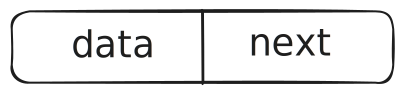
\includegraphics[width=0.6\textwidth]{./figure/pdf/cropped/singleStruct.pdf}
  \caption{单链表结构}
  \label{fig:singleLinkStruct}
\end{figure}
单链表的结构体定义如代码\ref{lst:singleLinkStruct}所示。
\begin{lstlisting}[language=C++, caption={单链表结构体定义}, label={lst:singleLinkStruct}]
  struct ListNode {
    int data;
    ListNode* next;
  };
\end{lstlisting}
单链表的基本操作包括插入、删除、查找和更新。以下是每种操作的详细说明:
建立单链表:

  头插法建立单链表

  1.首先创建一个头结点,将头结点的指针域指向 NULL。
  2.依次读入数据元素,创建新节点,将新节点的指针域指向头结点的下一个节点,再将头结点的指针域指向新节点。
  具体过程如图\ref{fig:headInsert}所示。
  \begin{figure}[h]
    \centering
    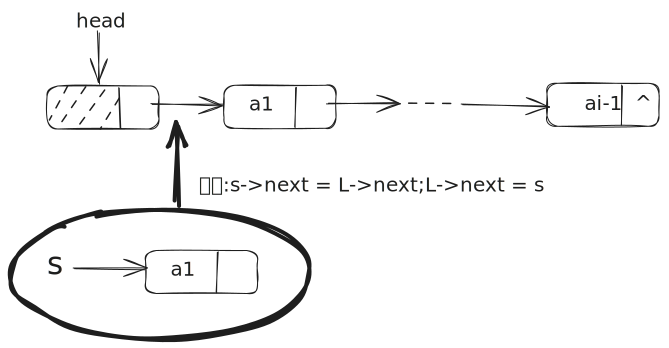
\includegraphics[width=1\textwidth]{./figure/pdf/cropped/headInsert.pdf}
    \caption{头插法建立单链表}
    \label{fig:headInsert}
  \end{figure}
  代码如代码\ref{lst:headInsert}所示。
  \begin{lstlisting}[language=C++, caption={头插法建立单链表示例代码}, label={lst:headInsert}]
    singleLink* createSingleLink() {
      int n, data;
      printf("请输入创建链表的节点个数:");
      scanf("%d", &n);
      SingleLink* L = (SingleLink*)malloc(sizeof(SingleLink));
      L->next = NULL;
      for (int i = 0; i < n; i++) {
        SingleLink* s = (singleLink*)malloc(sizeof(SingleLink));
        printf("请输入第%d个节点的值(int):", i + 1);
        scanf("%d", &data);
        s->data = data;
        s->next = NULL;
        s->next = L->next;
        L->next = s;
      }
      return L;
    }
    \end{lstlisting}
    该算法的总时间复杂度为 $O(n)$,空间复杂度为 $O(1)$。

    特点:头插法建立的单链表,新节点插入到链表的头部,逆序存储数据。

  尾插法建立单链表

  1.首先创建一个头结点,将头结点的指针域指向 NULL。
  2.依次读入数据元素,创建新节点,将新节点的指针域指向 NULL,再将尾结点的指针域指向新节点,再将新节点作为尾结点。
  具体过程如图\ref{fig:tailInsert}所示。
  \begin{figure}[h]
    \centering
    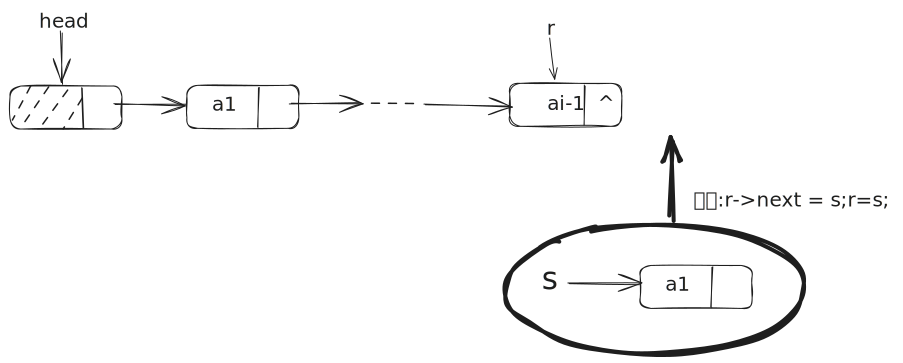
\includegraphics[width=1\textwidth]{./figure/pdf/cropped/tailInsert.pdf}
    \caption{尾插法建立单链表}
    \label{fig:tailInsert}
  \end{figure}
  代码如代码\ref{lst:tailInsert}所示。
  \begin{lstlisting}[language=C++, caption={尾插法建立单链表示例代码}, label={lst:tailInsert}]
    singleLink* createSingleLink() {
      int n, data;
      printf("请输入创建链表的节点个数:");
      scanf("%d", &n);
      SingleLink* L = (SingleLink*)malloc(sizeof(SingleLink));
      SingleLink* r = L;
      for (int i = 0; i < n; i++) {
        SingleLink* s = (singleLink*)malloc(sizeof(SingleLink));
        printf("请输入第%d个节点的值(int):", i + 1);
        scanf("%d", &data);
        s->data = data;
        s->next = NULL;
        r->next = s;
        r = s;
      }
      return L;
    }
    \end{lstlisting}
    该算法的总时间复杂度为 $O(n)$,空间复杂度为 $O(1)$。

    特点:尾插法建立的单链表,新节点插入到链表的尾部,顺序存储数据。

创建一个空链表

创建一个空链表,只需要创建一个头结点,将头结点的指针域指向 NULL。

代码如代码\ref{lst:createEmptySingleLink}所示。
\begin{lstlisting}[language=C++, caption={创建一个空链表示例代码}, label={lst:createEmptySingleLink}]
  singleLink* createEmptySingleLink() {
    SingleLink* L = (SingleLink*)malloc(sizeof(SingleLink));
    L->next = NULL;
    return L;
  }
\end{lstlisting}
该算法的总时间复杂度为 $O(1)$,空间复杂度为 $O(1)$。

特点:创建的链表为空,不包含任何数据元素。

输出单链表

输出单链表的所有数据元素,需要遍历链表的所有节点,并依次输出节点的数据域。

代码如代码\ref{lst:printSingleLink}所示。

\begin{lstlisting}[language=C++, caption={输出单链表示例代码}, label={lst:printSingleLink}]
void printSingleLink(SingleLink* L) {
  SingleLink* p = L->next;
  while (p != NULL) {
    printf("%d ", p->data);
    p = p->next;
  }
  printf("\n");
}
\end{lstlisting}
该算法的总时间复杂度为 $O(n)$,空间复杂度为 $O(1)$。

特点:输出单链表的所有数据元素。

输出单链表的长度

输出单链表的长度,需要遍历链表的所有节点,并统计节点的个数。

代码如代码\ref{lst:lengthSingleLink}所示。

\begin{lstlisting}[language=C++, caption={输出单链表长度示例代码}, label={lst:lengthSingleLink}]
int lengthSingleLink(SingleLink* L) {
  SingleLink* p = L->next;
  int length = 0;
  while (p != NULL) {
    length++;
    p = p->next;
  }
  return length;
}
\end{lstlisting}
该算法的总时间复杂度为 $O(n)$,空间复杂度为 $O(1)$。

特点:输出单链表的长度,即链表中数据元素的个数。

判断单链表是否为空

判断单链表是否为空,只需要判断头结点的指针域是否为 NULL。

代码如代码\ref{lst:isEmptySingleLink}所示。

\begin{lstlisting}[language=C++, caption={判断单链表是否为空示例代码}, label={lst:isEmptySingleLink}]
  bool isEmptySingleLink(SingleLink* L) {
    return L->next == NULL;
  }
  \end{lstlisting}
  该算法的总时间复杂度为 $O(1)$,空间复杂度为 $O(1)$。

  特点:判断单链表是否为空,即链表中是否包含数据元素。

查找单链表的第 $i$ 个元素

查找单链表的第 $i$ 个元素,需要遍历链表的所有节点,直到找到第 $i$ 个节点。

代码如代码\ref{lst:getSingleLink}所示。

\begin{lstlisting}[language=C++, caption={查找单链表的第 $i$ 个元素示例代码}, label={lst:getSingleLink}]
  int getSingleLink(SingleLink* L, int i) {
    SingleLink* p = L->next;
    int j = 1;
    while (p != NULL && j < i) {
      p = p->next;
      j++;
    }
    if (p == NULL || j > i) {
      printf("第%d个元素不存在", i);
      return -1;
    }
    return p->data;
  }
\end{lstlisting}
该算法的总时间复杂度为 $O(n)$,空间复杂度为 $O(1)$。

特点:查找单链表的第 $i$ 个元素,即链表中第 $i$ 个节点的数据元素。

删除单链表的第 $i$ 个元素

删除单链表的第 $i$ 个元素,需要遍历链表的所有节点,直到找到第 $i$ 个节点,然后删除该节点。

代码如代码\ref{lst:deleteSingleLink}所示。

\begin{lstlisting}[language=C++, caption={删除单链表的第 $i$ 个元素示例代码}, label={lst:deleteSingleLink}]
  void deleteSingleLink(SingleLink* L, int i) {
    SingleLink* p = L;
    for (int j = 0; j < i - 1; j++) {
      p = p->next;
    }
    SingleLink* q = p->next;
    p->next = q->next;
    free(q);
  }
  \end{lstlisting}
  该算法的总时间复杂度为 $O(n)$,空间复杂度为 $O(1)$。

  特点:删除单链表的第 $i$ 个元素,即删除链表中第 $i$ 个节点。

插入单链表的第 $i$ 个元素

插入单链表的第 $i$ 个元素,需要遍历链表的所有节点,直到找到第 $i$ 个节点,然后插入新节点。

代码如代码\ref{lst:insertSingleLink}所示。

\begin{lstlisting}[language=C++, caption={插入单链表的第 $i$ 个元素示例代码}, label={lst:insertSingleLink}]
void insertSingleLink(SingleLink* L, int i, int data) {
  SingleLink* p = L;
  for (int j = 0; j < i - 1; j++) {
    p = p->next;
  }
  SingleLink* s = (SingleLink*)malloc(sizeof(SingleLink));
  s->data = data;
  s->next = p->next;
  p->next = s;
}
\end{lstlisting}
该算法的总时间复杂度为 $O(n)$,空间复杂度为 $O(1)$。

特点:插入单链表的第 $i$ 个元素,即在链表中第 $i$ 个节点的位置插入新节点。
   



  \subsubsection{双链表}
  单链表只有指向下一个节点的指针,在某一些应用场合可能并不是那么方便,比如在删除某个节点时,需要找到该节点的前驱节点,而单链表并没有指向前驱节点的指针。双链表就是为了解决这个问题而设计的,它的每个节点有两个指针,一个指向前驱节点,一个指向后继节点。
  
  \textit{示例}:
  $L = \{\text{NULL} \leftrightarrow 1001 \leftrightarrow 1002 \leftrightarrow 1003 \leftrightarrow \text{NULL}\}$。

  双链表的结构如图\ref{fig:doubleLinkStruct}所示。双链表的结构由数据域、前驱指针和后继指针组成,其中数据域存储数据元素,前驱指针指向前一个节点,后继指针指向后一个节点。
  \begin{figure}[h]
    \centering
    
\includegraphics[width=0.6\textwidth]{./figure/pdf/cropped/doubleLinkStruct.pdf}
    \caption{双链表结构}
    \label{fig:doubleLinkStruct}
  \end{figure}

  双链表的结构体定义如代码\ref{lst:doubleLinkStruct}所示。
  \begin{lstlisting}[language=C++, caption={双链表结构体定义}, label={lst:doubleLinkStruct}]
    struct DLink {
      int data;
      DLink* pre;
      DLink* next;
    };
  \end{lstlisting}

  双链表的基本操作包括插入、删除、查找和更新。以下是每种操作的详细说明:

  \textbf{创建操作}:

  创建一个空的双链表,只需要创建一个头结点,将头结点的前驱指针和后继指针都指向 NULL。

  代码如代码\ref{lst:createEmptyDoubleLink}所示。
  \begin{lstlisting}[language=C++, caption={创建一个空双链表示例代码}, label={lst:createEmptyDoubleLink}]
    DLink* createEmptyDoubleLink() {
      DLink* L = (DLink*)malloc(sizeof(DLink));
      L->pre = NULL;
      L->next = NULL;
      return L;
    }
  \end{lstlisting}
  该算法的总时间复杂度为 $O(1)$,空间复杂度为 $O(1)$。

  特点:创建的双链表为空,不包含任何数据元素。

  \textbf{头插法}:

  头插法建立双链表,新节点插入到链表的头部。

  1.首先创建一个头结点,将头结点的前驱指针和后继指针都指向 NULL。

  2.依次读入数据元素,创建新节点,将新节点的前驱指针指向头结点,将新节点的后继指针指向头结点的后继节点,再将头结点的后继指针指向新节点,最后将新节点作为头结点的后继节点。

  具体过程如图\ref{fig:headInsertDouble}所示。
  \begin{figure}[h]
    \centering
    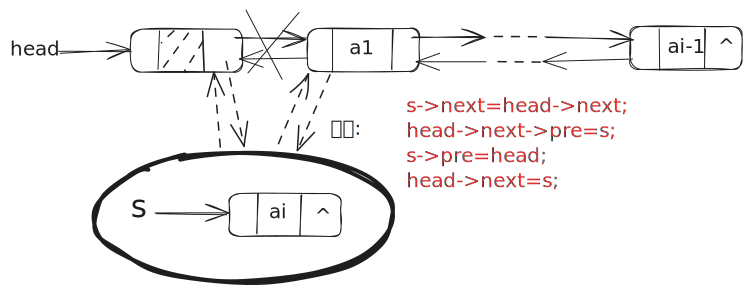
\includegraphics[width=1\textwidth]{./figure/pdf/cropped/headInsertDL.pdf}
    \caption{头插法建立双链表}
    \label{fig:headInsertDouble}
  \end{figure}
  代码如代码\ref{lst:headInsertDouble}所示。
  \begin{lstlisting}[language=C++, caption={头插法建立双链表示例代码}, label={lst:headInsertDouble}]
    DLink* createDoubleLink() {
      int n, data;
      printf("请输入创建链表的节点个数:");
      scanf("%d", &n);
      DLink* L = (DLink*)malloc(sizeof(DLink));
      L->pre = NULL;
      L->next = NULL;
      for (int i = 0; i < n; i++) {
        DLink* s = (DLink*)malloc(sizeof(DLink));
        printf("请输入第%d个节点的值(int):", i + 1);
        scanf("%d", &data);
        s->data = data;
        s->pre = L;
        s->next = L->next;
        L->next = s;
      }
      return L;
    }
  \end{lstlisting}
  该算法的总时间复杂度为 $O(n)$,空间复杂度为 $O(1)$。
  \textbf{尾插法}:
  尾插法建立双链表,新节点插入到链表的尾部。

  1.首先创建一个头结点,将头结点的前驱指针和后继指针都指向 NULL。

  2.依次读入数据元素,创建新节点,将新节点的前驱指针指向尾结点,将新节点的后继指针指向 NULL,再将尾结点的后继指针指向新节点,最后将新节点作为尾结点。

  具体过程如图\ref{fig:tailInsertDouble}所示。
  \begin{figure}[h]
    \centering
    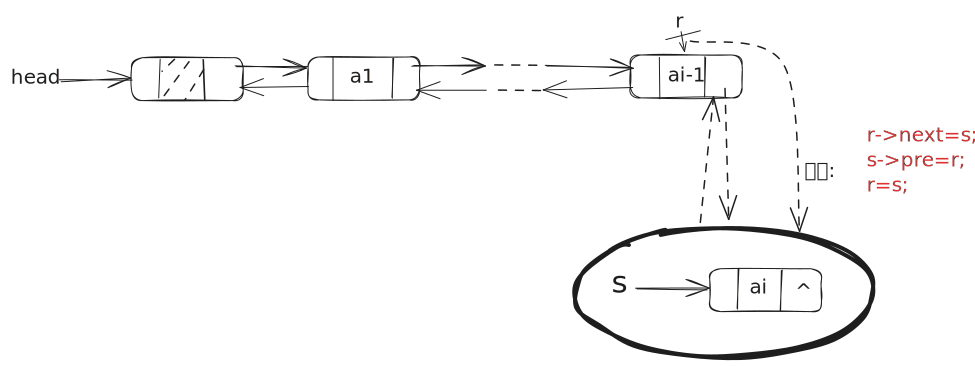
\includegraphics[width=1\textwidth]{./figure/pdf/cropped/tailInsertDL.pdf}
    \caption{尾插法建立双链表}
    \label{fig:tailInsertDouble}
  \end{figure}
  代码如代码\ref{lst:tailInsertDouble}所示。

  \begin{lstlisting}[language=C++, caption={尾插法建立双链表示例代码}, label={lst:tailInsertDouble}]
    DLink* createDoubleLink() {
      int n, data;
      printf("请输入创建链表的节点个数:");
      scanf("%d", &n);
      DLink* L = (DLink*)malloc(sizeof(DLink));
      DLink* r = L;
      for (int i = 0; i < n; i++) {
        DLink* s = (DLink*)malloc(sizeof(DLink));
        printf("请输入第%d个节点的值(int):", i + 1);
        scanf("%d", &data);
        s->data = data;
        s->pre = r;
        s->next = NULL;
        r->next = s;
        r = s;
      }
      return L;
    }
  \end{lstlisting}
  该算法的总时间复杂度为 $O(n)$,空间复杂度为 $O(1)$。

  特点:尾插法建立的双链表,新节点插入到链表的尾部,顺序存储数据。

  \textbf{输出操作}:

  输出双链表的所有数据元素,需要遍历链表的所有节点,并依次输出节点的数据域。

  代码如代码\ref{lst:printDoubleLink}所示。

  \begin{lstlisting}[language=C++, caption={输出双链表示例代码}, label={lst:printDoubleLink}]
    void printDoubleLink(DLink* L) {
      DLink* p = L->next;
      while (p != NULL) {
        printf("%d ", p->data);
        p = p->next;
      }
      printf("\n");
    }
  \end{lstlisting}

  该算法的总时间复杂度为 $O(n)$,空间复杂度为 $O(1)$。

  特点:输出双链表的所有数据元素。

  \textbf{输出双链表的长度}:

  输出双链表的长度,需要遍历链表的所有节点,并统计节点的个数。

  代码如代码\ref{lst:lengthDoubleLink}所示。

  \begin{lstlisting}[language=C++, caption={输出双链表长度示例代码}, label={lst:lengthDoubleLink}]
    int lengthDoubleLink(DLink* L) {
      DLink* p = L->next;
      int length = 0;
      while (p != NULL) {
        length++;
        p = p->next;
      }
      return length;
    }
  \end{lstlisting}

  该算法的总时间复杂度为 $O(n)$,空间复杂度为 $O(1)$。

  特点:输出双链表的长度,即链表中数据元素的个数。

  \textbf{判断双链表是否为空}:

  判断双链表是否为空,只需要判断头结点的后继指针是否为 NULL。

  代码如代码\ref{lst:isEmptyDoubleLink}所示。

  \begin{lstlisting}[language=C++, caption={判断双链表是否为空示例代码}, label={lst:isEmptyDoubleLink}]
    bool isEmptyDoubleLink(DLink* L) {
      return L->next == NULL;
    }
  \end{lstlisting}

  该算法的总时间复杂度为 $O(1)$,空间复杂度为 $O(1)$。

  特点:判断双链表是否为空,即链表中是否包含数据元素。

  \textbf{查找双链表的第 $i$ 个元素}:

  查找双链表的第 $i$ 个元素,需要遍历链表的所有节点,直到找到第 $i$ 个节点。

  代码如代码\ref{lst:getDoubleLink}所示。

  \begin{lstlisting}[language=C++, caption={查找双链表的第 $i$ 个元素示例代码}, label={lst:getDoubleLink}]
    int getDoubleLink(DLink* L, int i) {
      DLink* p = L->next;
      int j = 1;
      while (p != NULL && j < i) {
        p = p->next;
        j++;
      }
      if (p == NULL || j > i) {
        printf("第%d个元素不存在", i);
        return -1;
      }
      return p->data;
    }
  \end{lstlisting}

  该算法的总时间复杂度为 $O(n)$,空间复杂度为 $O(1)$。

  特点:查找双链表的第 $i$ 个元素,即链表中第 $i$ 个节点的数据元素。

  \textbf{删除双链表的第 $i$ 个元素}:

  删除双链表的第 $i$ 个元素,需要遍历链表的所有节点,直到找到第 $i$ 个节点,然后删除该节点。

  代码如代码\ref{lst:deleteDoubleLink}所示。

  \begin{lstlisting}[language=C++, caption={删除双链表的第 $i$ 个元素示例代码}, label={lst:deleteDoubleLink}]
    void deleteDoubleLink(DLink* L, int i) {
      DLink* p = L;
      for (int j = 0; j < i - 1; j++) {
        p = p->next;
      }
      DLink* q = p->next;
      p->next = q->next;
      if (q->next != NULL) {
        q->next->pre = p;
      }
      free(q);
    }
  \end{lstlisting}

  该算法的总时间复杂度为 $O(n)$,空间复杂度为 $O(1)$。

  特点:删除双链表的第 $i$ 个元素,即删除链表中第 $i$ 个节点。

  \textbf{插入双链表的第 $i$ 个元素}:

  插入双链表的第 $i$ 个元素,需要遍历链表的所有节点,直到找到第 $i$ 个节点,然后插入新节点。

  其中删除操作如图\ref{fig:deleteDoubleLink}所示。

  \begin{figure}[h]
    \centering
    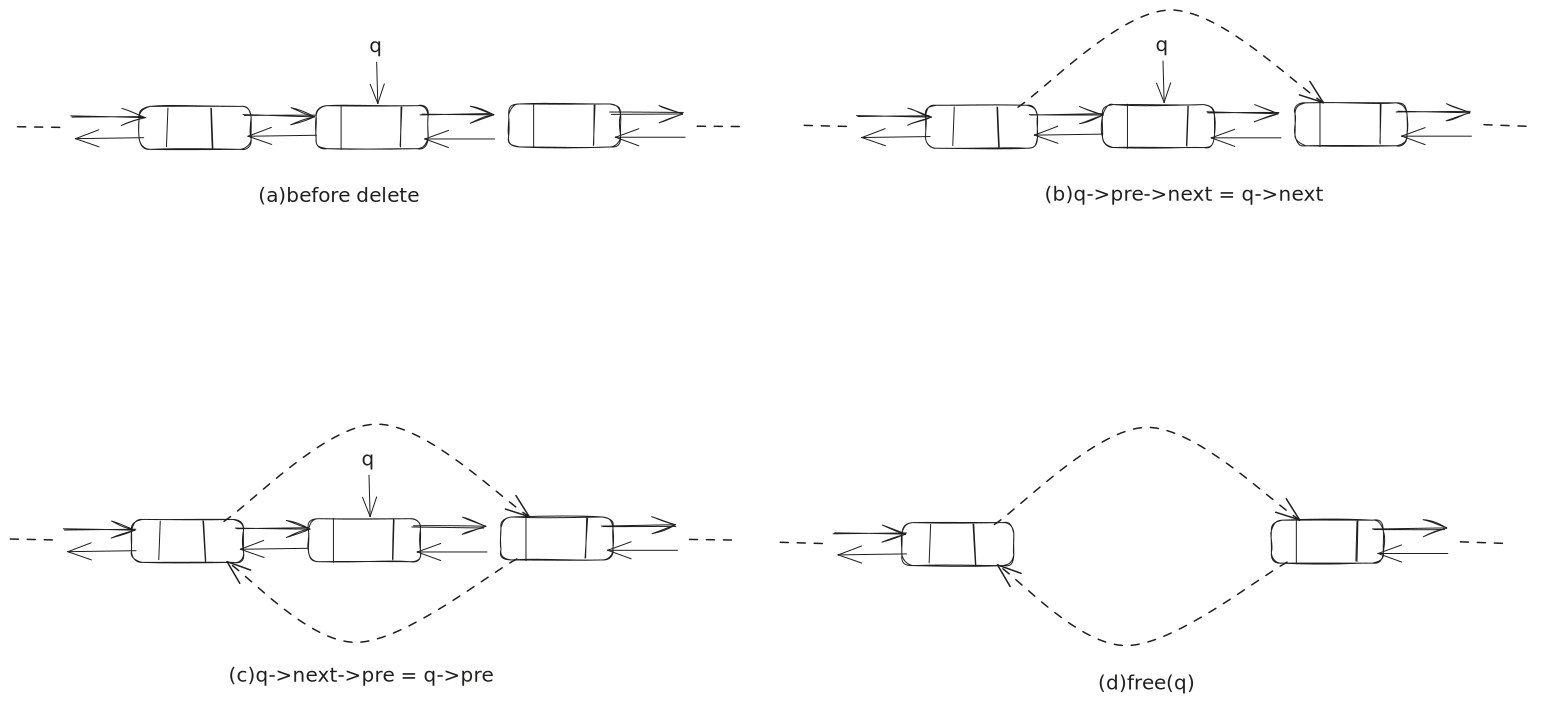
\includegraphics[width=1\textwidth]{./figure/pdf/cropped/deleteDL.pdf}
    \caption{删除双链表的第 $i$ 个元素}
    \label{fig:deleteDoubleLink}
  \end{figure}

  代码如代码\ref{lst:insertDoubleLink}所示。

  \begin{lstlisting}[language=C++, caption={插入双链表的第 $i$ 个元素示例代码}, label={lst:insertDoubleLink}]
    void insertDoubleLink(DLink* L, int i, int data) {
      DLink* p = L;
      for (int j = 0; j < i - 1; j++) {
        p = p->next;
      }
      DLink* s = (DLink*)malloc(sizeof(DLink));
      s->data = data;
      s->pre = p;
      s->next = p->next;
      if (p->next != NULL) {
        p->next->pre = s;
      }
      p->next = s;
    }

  \end{lstlisting}

  该算法的总时间复杂度为 $O(n)$,空间复杂度为 $O(1)$。

  特点:插入双链表的第 $i$ 个元素,即在链表中第 $i$ 个节点的位置插入新节点。

  \textbf{p结点之后插入结点s}:

  过程如图\ref{fig:insertAfterDoubleLink}所示。

  \begin{figure}[h]
    \centering
    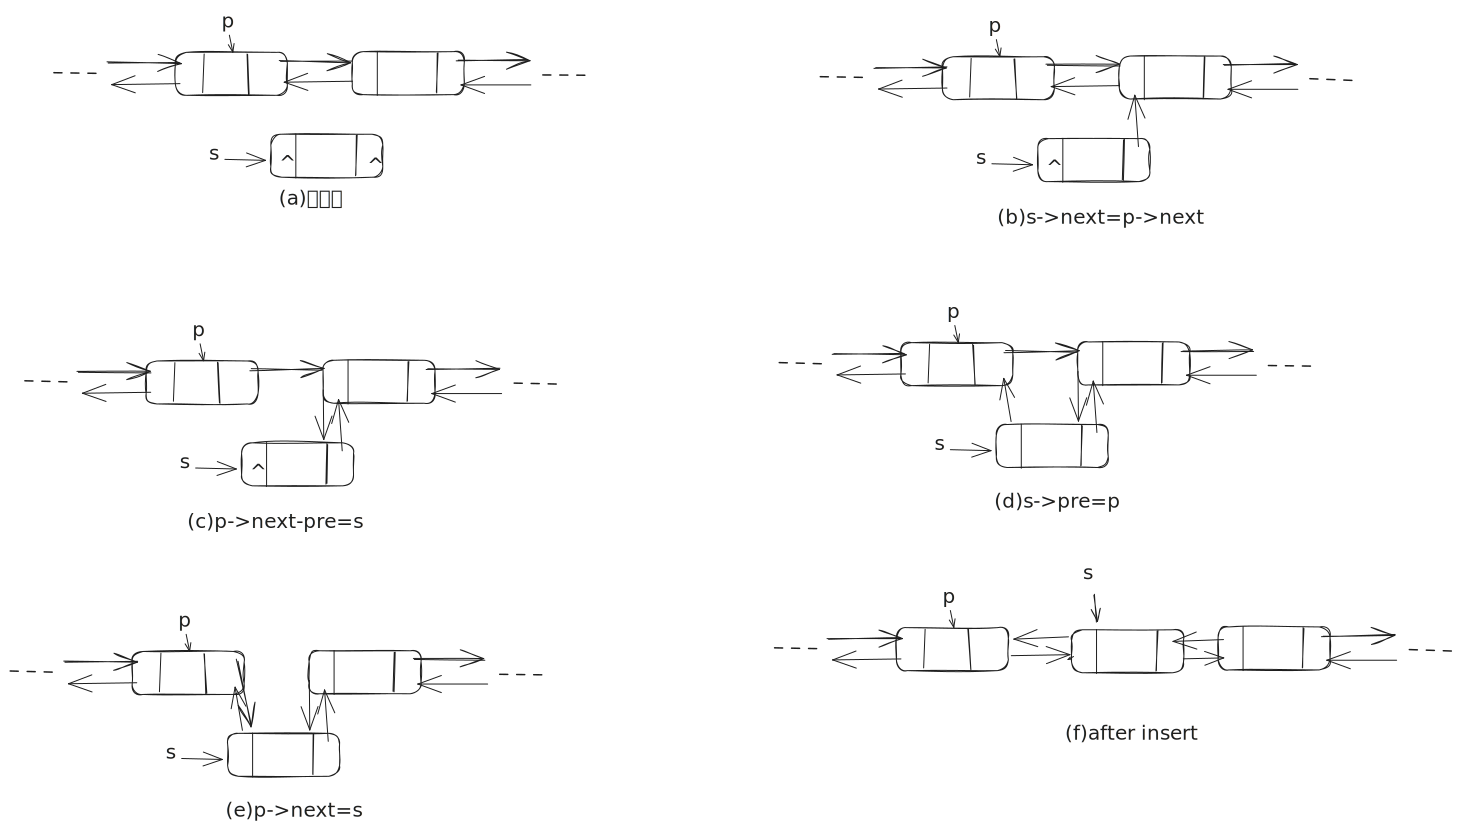
\includegraphics[width=1\textwidth]{./figure/pdf/cropped/insertDL.pdf}
    \caption{p结点之后插入结点s}
    \label{fig:insertAfterDoubleLink}
  \end{figure}
  代码如代码\ref{lst:insertAfterDoubleLink}所示。

  \begin{lstlisting}[language=C++, caption={p结点之后插入结点s示例代码}, label={lst:insertAfterDoubleLink}]
    void insertAfterDoubleLink(DLink* p, DLink* s) {
      s->pre = p;
      s->next = p->next;
      if (p->next != NULL) {
        p->next->pre = s;
      }
      p->next = s;
    }
  \end{lstlisting}

  该算法的总时间复杂度为 $O(1)$,空间复杂度为 $O(1)$。

  特点:在双链表中结点 p 之后插入结点 s。



  \subsubsection{循环链表\textbackslash\&静态链表}
  循环链表是链表的一种,最后一个节点的指针指向第一个节点,形成一个环。
  \textit{示例}:
  $L = \{1001 \rightarrow 1002 \rightarrow 1003 \rightarrow 1001\}$。

  \textbf{循环单链表}:

  循环单链表和单链表的区别在于,循环单链表的尾结点指针指向头结点。

  其结构如图\ref{fig:cycleSingleLink}所示。

  \begin{figure}[h]
    \centering
    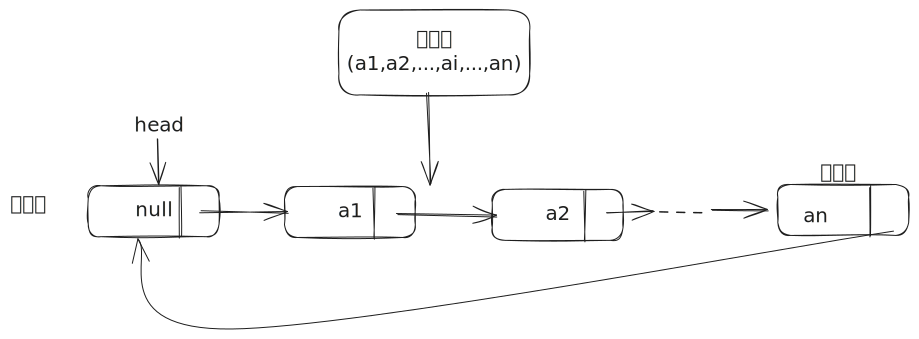
\includegraphics[width=0.6\textwidth]{./figure/pdf/cropped/cycleSLink.pdf}
    \caption{循环单链表结构}
    \label{fig:cycleSingleLink}
  \end{figure}

  \textbf{循环双链表}:

  循环双链表和双链表的区别在于,循环双链表的头结点的前驱指针指向尾结点,尾结点的后继指针指向头结点。

  其结构如图\ref{fig:cycleDoubleLink}所示。

  \begin{figure}[h]
    \centering
    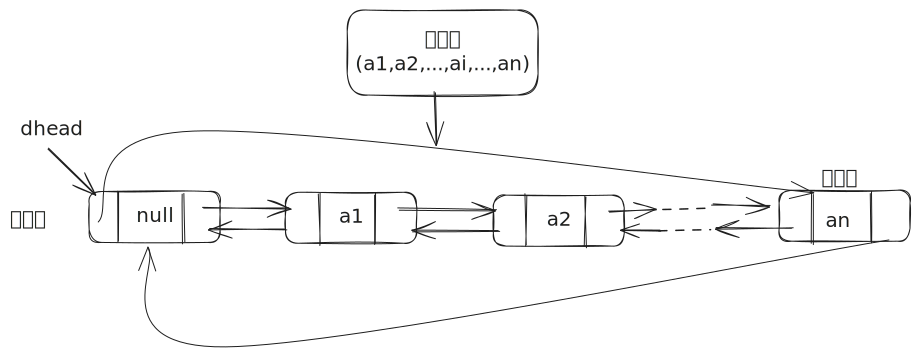
\includegraphics[width=0.6\textwidth]{./figure/pdf/cropped/cycleDLink.pdf}
    \caption{循环双链表结构}
    \label{fig:cycleDoubleLink}
  \end{figure}


  静态链表是使用数组模拟链表的一种实现方式,每个数组元素包含数据域和指针域。与前面所讲的链表不同,静态链表的指针域
  存储的是数组的索引,而不是指向下一个节点的指针。静态链表和顺序表一样,使用数组存储数据元素,但是静态链表可以更好地支持插入和删除操作。

  如图\ref{fig:staticLink}所示,静态链表的结构由数据域和指针域组成,其中数据域存储数据元素,指针域存储数组的索引。

  \begin{figure}[h]
    \centering
    \includegraphics[width=1\textwidth]{./figure/pdf/cropped/staticLink.pdf}
    \caption{静态链表结构}
    \label{fig:staticLink}
  \end{figure}

 数组的第一个元素不存储数据,它的指针域存储第一个数据元素的索引,最后一个元素的指针域存储下一个空闲位置的索引。最后一个
 元素的指针域值为-1。

  \section{顺序表与链表的比较}
  \begin{itemize}
      \item \textbf{存储方式}:顺序表使用数组存储数据元素,链表使用指针存储数据元素。
      \item \textbf{插入和删除}:顺序表插入和删除操作需要移动元素,时间复杂度为 $O(n)$,链表插入和删除操作只需要修改指针,时间复杂度为 $O(1)$。
      \item \textbf{空间复杂度}:顺序表的空间复杂度为 $O(n)$,链表的空间复杂度为 $O(n)$。
      \item \textbf{访问速度}:顺序表的访问速度快,时间复杂度为 $O(1)$,链表的访问速度慢,时间复杂度为 $O(n)$。
  \end{itemize}




\textit{总结}:顺序表适合需要频繁访问的场景,而链表适合需要频繁插入和删除的场景。

\chapter{栈与队列}
从组成元素的逻辑关系来看,栈和队列都属于线性结构.栈和队列与线性表的不同之处在于它们的相关运算具有一些特殊性.
更准确地说,一般线性表上的插入/删除运算不受限制,而栈和队列上的插入 删除运算均会受到某种特殊限制,
因此栈和队列也称为操作受限的线性表.
\section{栈}

\subsection{栈的定义}

栈是一种特殊的线性表,只能在表的一端进行插入和删除操作。栈的插入操作称为入栈,删除操作称为出栈。栈的特点是后进先出,即最后入栈的元素最先出栈。

如图\ref{fig:stack}所示,栈的结构由栈顶和栈底组成,栈顶指向栈顶元素,栈底指向栈底元素。

\begin{figure}[h]
  \centering
  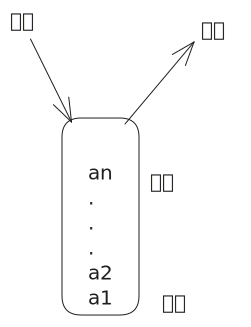
\includegraphics[width=0.2\textwidth]{./figure/pdf/cropped/stack.pdf}
  \caption{栈结构}
  \label{fig:stack}
\end{figure}

相关术语:

\begin{itemize}
  \item \textbf{栈顶}:栈顶是栈中最后一个元素。
  \item \textbf{栈底}:栈底是栈中第一个元素。
  \item \textbf{空栈}:栈中不包含任何元素。
  \item \textbf{满栈}:栈中包含的元素个数等于栈的最大容量。
  \item \textbf{栈的大小}:栈中包含的元素个数。
  \item \textbf{栈的容量}:栈的最大容量。
  \item \textbf{栈的压入}:将元素压入栈中。
  \item \textbf{栈的弹出}:将元素从栈中弹出。
  \end{itemize}

栈的特点:

\begin{itemize}
  \item 栈是一种特殊的线性表,只能在表的一端进行插入和删除操作。
  \item 栈的插入操作称为入栈,删除操作称为出栈。
  \item 栈的特点是后进先出,即最后入栈的元素最先出栈。
\end{itemize}
\subsection{栈的操作}

栈的基本操作包括创建、销毁、压入、弹出、获取栈顶元素、判断栈是否为空、判断栈是否为满、获取栈的大小和获取栈的容量。

\begin{itemize}
  \item \textbf{创建操作}:创建一个空栈。
  \item \textbf{销毁操作}:销毁栈。
  \item \textbf{压入操作}:将元素压入栈中。
  \item \textbf{弹出操作}:将元素从栈中弹出。
  \item \textbf{获取栈顶元素}:获取栈顶元素。
  \item \textbf{判断栈是否为空}:判断栈中是否包含元素。
  \item \textbf{判断栈是否为满}:判断栈中是否包含元素。
  \item \textbf{获取栈的大小}:获取栈中包含的元素个数。
  \item \textbf{获取栈的容量}:获取栈的最大容量。
  \item \textbf{清空栈}:清空栈中的所有元素。
  \item \textbf{遍历栈}:遍历栈中的所有元素。
\end{itemize}


\subsection{顺序栈}

顺序栈是使用数组实现的栈,栈的大小是固定的,栈的容量是数组的大小。

顺序栈的结构体定义如代码\ref{lst:seqStackStruct}所示。

\begin{lstlisting}[language=C++, caption={顺序栈结构体定义}, label={lst:seqStackStruct}]
  struct SeqStack {
    int* data;//栈的数据元素
    int top;//栈顶指针
    int capacity;//栈的容量
  };
\end{lstlisting}

顺序栈的存放过程如图\ref{fig:seqStack}所示。

\begin{figure}[h]
  \centering
  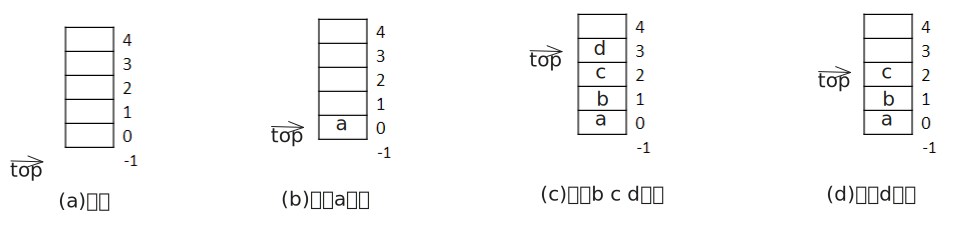
\includegraphics[width=1\textwidth]{./figure/pdf/cropped/processOfSeqStack.pdf}
  \caption{顺序栈存放过程}
  \label{fig:seqStack}
\end{figure}

顺序栈的基本操作包括创建、销毁、压入、弹出、获取栈顶元素、判断栈是否为空、判断栈是否为满、获取栈的大小和获取栈的容量。

\textbf{创建操作}:

创建一个空的顺序栈,需要为栈分配内存空间,并初始化栈的大小、栈的容量和栈顶指针。

代码如代码\ref{lst:createSeqStack}所示。

\begin{lstlisting}[language=C++, caption={创建一个空顺序栈示例代码}, label={lst:createSeqStack}]
  SeqStack* createSeqStack(int capacity) {
    SeqStack* S = (SeqStack*)malloc(sizeof(SeqStack));
    S->data = (int*)malloc(sizeof(int) * capacity);
    S->top = -1;
    S->capacity = capacity;
    return S;
  }

\end{lstlisting}

该算法的总时间复杂度为 $O(1)$,空间复杂度为 $O(n)$。

特点:创建的顺序栈为空,不包含任何数据元素。

\textbf{销毁操作}:

销毁顺序栈,需要释放栈的内存空间。

代码如代码\ref{lst:destroySeqStack}所示。

\begin{lstlisting}[language=C++, caption={销毁顺序栈示例代码}, label={lst:destroySeqStack}]
  void destroySeqStack(SeqStack* S) {
    free(S->data);
    free(S);
  }
\end{lstlisting}

该算法的总时间复杂度为 $O(1)$,空间复杂度为 $O(1)$。

特点:销毁顺序栈,释放栈的内存空间。

\textbf{判满操作}:

判断顺序栈是否为满,即栈中包含的元素个数等于栈的容量。

代码如代码\ref{lst:isFullSeqStack}所示。

\begin{lstlisting}[language=C++, caption={判断顺序栈是否为满示例代码}, label={lst:isFullSeqStack}]
  bool isFullSeqStack(SeqStack* S) {
    return S->top == S->capacity - 1;
  }

\end{lstlisting}

该算法的总时间复杂度为 $O(1)$,空间复杂度为 $O(1)$。

特点:判断顺序栈是否为满,即栈中包含的元素个数等于栈的容量。

\textbf{判空操作}:

判断顺序栈是否为空,即栈中不包含任何元素。

代码如代码\ref{lst:isEmptySeqStack}所示。

\begin{lstlisting}[language=C++, caption={判断顺序栈是否为空示例代码}, label={lst:isEmptySeqStack}]
  bool isEmptySeqStack(SeqStack* S) {
    return S->top == -1;
  }

\end{lstlisting}

该算法的总时间复杂度为 $O(1)$,空间复杂度为 $O(1)$。

特点:判断顺序栈是否为空,即栈中不包含任何元素。

\textbf{压入操作}:

将元素压入顺序栈中,即将元素放入栈顶。

代码如代码\ref{lst:pushSeqStack}所示。

\begin{lstlisting}[language=C++, caption={压入顺序栈示例代码}, label={lst:pushSeqStack}]
  void pushSeqStack(SeqStack* S, int data) {
    if (isFullSeqStack(S)) {
      printf("栈已满,无法压入元素\n");
      return;
    }
    S->data[++S->top] = data;
  }

\end{lstlisting}

该算法的总时间复杂度为 $O(1)$,空间复杂度为 $O(1)$。

特点:将元素压入顺序栈中,即将元素放入栈顶。

\textbf{弹出操作}:

将元素从顺序栈中弹出,即将栈顶元素删除。

代码如代码\ref{lst:popSeqStack}所示。

\begin{lstlisting}[language=C++, caption={弹出顺序栈示例代码}, label={lst:popSeqStack}]
  void popSeqStack(SeqStack* S) {
    if (isEmptySeqStack(S)) {
      printf("栈为空,无法弹出元素\n");
      return;
    }
    S->top--;
  }

\end{lstlisting}

该算法的总时间复杂度为 $O(1)$,空间复杂度为 $O(1)$。

特点:将元素从顺序栈中弹出,即将栈顶元素删除。

\textbf{获取栈顶元素}:

获取顺序栈的栈顶元素,即获取栈顶元素的值。

代码如代码\ref{lst:getTopSeqStack}所示。

\begin{lstlisting}[language=C++, caption={获取顺序栈的栈顶元素示例代码}, label={lst:getTopSeqStack}]
  int getTopSeqStack(SeqStack* S) {
    if (isEmptySeqStack(S)) {
      printf("栈为空,无法获取栈顶元素\n");
      return -1;
    }
    return S->data[S->top];
  }

\end{lstlisting}

该算法的总时间复杂度为 $O(1)$,空间复杂度为 $O(1)$。

特点:获取顺序栈的栈顶元素,即获取栈顶元素的值。

\textbf{获取栈的大小}:

获取顺序栈的大小,即获取栈中包含的元素个数。

代码如代码\ref{lst:sizeSeqStack}所示。

\begin{lstlisting}[language=C++, caption={获取顺序栈的大小示例代码}, label={lst:sizeSeqStack}]
  int sizeSeqStack(SeqStack* S) {
    return S->top + 1;
  }

\end{lstlisting}

该算法的总时间复杂度为 $O(1)$,空间复杂度为 $O(1)$。

特点:获取顺序栈的大小,即获取栈中包含的元素个数。

\textbf{获取栈的容量}:

获取顺序栈的容量,即获取栈的最大容量。

代码如代码\ref{lst:capacitySeqStack}所示。

\begin{lstlisting}[language=C++, caption={获取顺序栈的容量示例代码}, label={lst:capacitySeqStack}]
  int capacitySeqStack(SeqStack* S) {
    return S->capacity;
  }

\end{lstlisting}

该算法的总时间复杂度为 $O(1)$,空间复杂度为 $O(1)$。

特点:获取顺序栈的容量,即获取栈的最大容量。

\textbf{清空栈}:

清空顺序栈,即将栈中的所有元素删除。

代码如代码\ref{lst:clearSeqStack}所示。

\begin{lstlisting}[language=C++, caption={清空顺序栈示例代码}, label={lst:clearSeqStack}]
  void clearSeqStack(SeqStack* S) {
    S->top = -1;
  }

\end{lstlisting}

该算法的总时间复杂度为 $O(1)$,空间复杂度为 $O(1)$。

特点:清空顺序栈,即将栈中的所有元素删除。

\textbf{遍历栈}:

遍历顺序栈,即输出栈中的所有元素。

代码如代码\ref{lst:traverseSeqStack}所示。

\begin{lstlisting}[language=C++, caption={遍历顺序栈示例代码}, label={lst:traverseSeqStack}]
  void traverseSeqStack(SeqStack* S) {
    for (int i = 0; i <= S->top; i++) {
      printf("%d ", S->data[i]);
    }
    printf("\n");
  }

\end{lstlisting}

该算法的总时间复杂度为 $O(n)$,空间复杂度为 $O(1)$。

特点:遍历顺序栈,即输出栈中的所有元素。




\subsection{链栈}

栈是线性表的特例,线性表的存储结构还有链式存储结构,因此栈也可以使用链式存储结构实现,称为链栈.

链栈的结构体定义如代码\ref{lst:linkStackStruct}所示。

\begin{lstlisting}[language=C++, caption={链栈结构体定义}, label={lst:linkStackStruct}]
  struct LinkStack {
    int data;//栈的数据元素
    LinkStack* next;//栈的下一个元素
  };
\end{lstlisting}

链栈结构如图\ref{fig:linkStack}所示。

\begin{figure}[h]
  \centering
  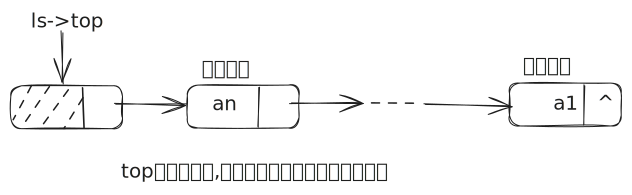
\includegraphics[width=1\textwidth]{./figure/pdf/cropped/linkStack.pdf}
  \caption{链栈}
  \label{fig:linkStack}
\end{figure}

我们可以发现,链栈的结构与单链表的结构相似,只是链栈的操作受到了限制,只能在栈顶进行插入和删除操作。

链栈的基本操作包括创建、销毁、压入、弹出、获取栈顶元素、判断栈是否为空、获取栈的大小和遍历栈。

\textbf{创建操作}:

创建一个空链栈,需要为栈分配内存空间,并初始化栈顶指针。

代码如代码\ref{lst:createLinkStack}所示。

\begin{lstlisting}[language=C++, caption={创建一个空链栈示例代码}, label={lst:createLinkStack}]
  LinkStack* createLinkStack() {
    LinkStack* S = (LinkStack*)malloc(sizeof(LinkStack));
    S->next = NULL;
    return S;
  }

\end{lstlisting}

该算法的总时间复杂度为 $O(1)$,空间复杂度为 $O(1)$。

特点:创建的链栈为空,不包含任何数据元素。

\textbf{销毁操作}:

销毁链栈,需要释放栈的内存空间。

代码如代码\ref{lst:destroyLinkStack}所示。

\begin{lstlisting}[language=C++, caption={销毁链栈示例代码}, label={lst:destroyLinkStack}]
  void destroyLinkStack(LinkStack* S) {
    LinkStack* p = S;
    while (p != NULL) {
      LinkStack* q = p;
      p = p->next;
      free(q);
    }
  }

\end{lstlisting}

该算法的总时间复杂度为 $O(n)$,空间复杂度为 $O(1)$。

特点:销毁链栈,释放栈的内存空间。

\textbf{判空操作}:

判断链栈是否为空,即栈中不包含任何元素。

代码如代码\ref{lst:isEmptyLinkStack}所示。

\begin{lstlisting}[language=C++, caption={判断链栈是否为空示例代码}, label={lst:isEmptyLinkStack}]
  bool isEmptyLinkStack(LinkStack* S) {
    return S->next == NULL;
  }

\end{lstlisting}

该算法的总时间复杂度为 $O(1)$,空间复杂度为 $O(1)$。

特点:判断链栈是否为空,即栈中不包含任何元素。

\textbf{压入操作}:

将元素压入链栈中,即将元素放入栈顶。

代码如代码\ref{lst:pushLinkStack}所示。

\begin{lstlisting}[language=C++, caption={压入链栈示例代码}, label={lst:pushLinkStack}]
  void pushLinkStack(LinkStack* S, int data) {
    LinkStack* p = (LinkStack*)malloc(sizeof(LinkStack));
    p->data = data;
    p->next = S->next;
    S->next = p;
  }

\end{lstlisting}

该算法的总时间复杂度为 $O(1)$,空间复杂度为 $O(1)$。

特点:将元素压入链栈中,即将元素放入栈顶。

\textbf{弹出操作}:

将元素从链栈中弹出,即将栈顶元素删除。

代码如代码\ref{lst:popLinkStack}所示。

\begin{lstlisting}[language=C++, caption={弹出链栈示例代码}, label={lst:popLinkStack}]
  void popLinkStack(LinkStack* S) {
    if (isEmptyLinkStack(S)) {
      printf("栈为空,无法弹出元素\n");
      return;
    }
    LinkStack* p = S->next;
    S->next = p->next;
    free(p);
  }

\end{lstlisting}

该算法的总时间复杂度为 $O(1)$,空间复杂度为 $O(1)$。

特点:将元素从链栈中弹出,即将栈顶元素删除。

\textbf{获取栈顶元素}:

获取链栈的栈顶元素,即获取栈顶元素的值。

代码如代码\ref{lst:getTopLinkStack}所示。

\begin{lstlisting}[language=C++, caption={获取链栈的栈顶元素示例代码}, label={lst:getTopLinkStack}]
  int getTopLinkStack(LinkStack* S) {
    if (isEmptyLinkStack(S)) {
      printf("栈为空,无法获取栈顶元素\n");
      return -1;
    }
    return S->next->data;
  }

\end{lstlisting}

该算法的总时间复杂度为 $O(1)$,空间复杂度为 $O(1)$。

特点:获取链栈的栈顶元素,即获取栈顶元素的值。

\textbf{遍历栈}:

遍历链栈,即输出栈中的所有元素。

代码如代码\ref{lst:traverseLinkStack}所示。

\begin{lstlisting}[language=C++, caption={遍历链栈示例代码}, label={lst:traverseLinkStack}]
  void traverseLinkStack(LinkStack* S) {
    LinkStack* p = S->next;
    while (p != NULL) {
      printf("%d ", p->data);
      p = p->next;
    }
    printf("\n");
  }

\end{lstlisting}

该算法的总时间复杂度为 $O(n)$,空间复杂度为 $O(1)$。

特点:遍历链栈,即输出栈中的所有元素。



\subsection{共享栈}

共享栈是两个栈共享一个存储空间的栈,两个栈的栈底分别位于共享空间的两端,两个栈的栈顶向中间延伸。

共享栈的结构如图\ref{fig:sharedStack}所示。

\begin{figure}[h]
  \centering
  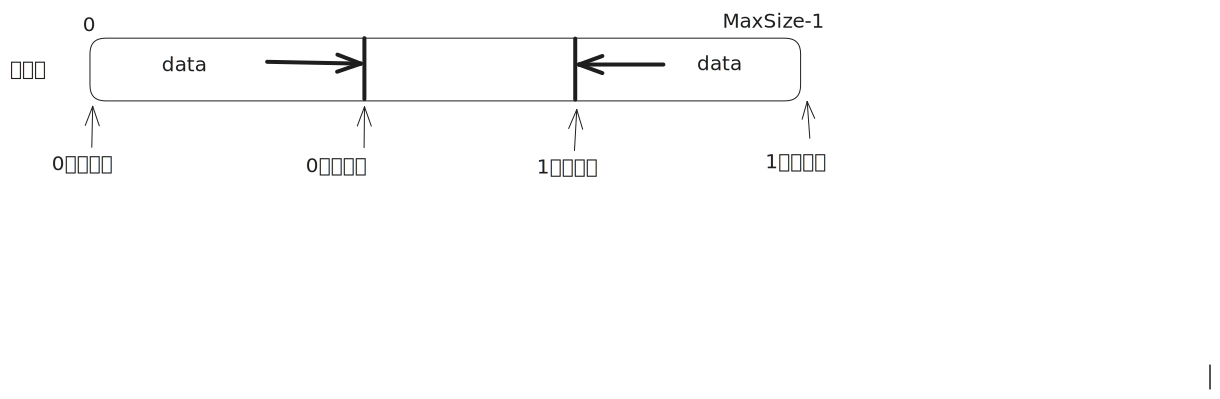
\includegraphics[width=1\textwidth]{./figure/pdf/cropped/shareStack.pdf}
  \caption{共享栈}
  \label{fig:sharedStack}
\end{figure}


共享栈的结构体定义如代码\ref{lst:sharedStackStruct}所示。

\begin{lstlisting}[language=C++, caption={共享栈结构体定义}, label={lst:sharedStackStruct}]
  struct SharedStack {
    int* data;//栈的数据元素
    int top1;//栈1的栈顶指针
    int top2;//栈2的栈顶指针
    int capacity;//栈的容量
  };
\end{lstlisting}

共享栈的基本操作包括创建、销毁、压入、弹出、获取栈顶元素、判断栈是否为空、判断栈是否为满、获取栈的大小和获取栈的容量。

\textbf{创建操作}:

创建一个空共享栈,需要为栈分配内存空间,并初始化栈的大小、栈的容量和栈顶指针。

代码如代码\ref{lst:createSharedStack}所示。

\begin{lstlisting}[language=C++, caption={创建一个空共享栈示例代码}, label={lst:createSharedStack}]
  SharedStack* createSharedStack(int capacity) {
    SharedStack* S = (SharedStack*)malloc(sizeof(SharedStack));
    S->data = (int*)malloc(sizeof(int) * capacity);
    S->top1 = -1;
    S->top2 = capacity;
    S->capacity = capacity;
    return S;
  }

\end{lstlisting}

该算法的总时间复杂度为 $O(1)$,空间复杂度为 $O(1)$。

特点:创建的共享栈为空,不包含任何数据元素。

\textbf{销毁操作}:

销毁共享栈,需要释放栈的内存空间。

代码如代码\ref{lst:destroySharedStack}所示。

\begin{lstlisting}[language=C++, caption={销毁共享栈示例代码}, label={lst:destroySharedStack}]
  void destroySharedStack(SharedStack* S) {
    free(S->data);
    free(S);
  }

\end{lstlisting}

该算法的总时间复杂度为 $O(1)$,空间复杂度为 $O(1)$。

特点:销毁共享栈,释放栈的内存空间。

\textbf{判空操作}:

判断共享栈是否为空,即栈中不包含任何元素。

代码如代码\ref{lst:isEmptySharedStack}所示。

\begin{lstlisting}[language=C++, caption={判断共享栈是否为空示例代码}, label={lst:isEmptySharedStack}]
  bool isEmptySharedStack(SharedStack* S, int stackNumber) {
    if (stackNumber == 1) {
      return S->top1 == -1;
    } else if (stackNumber == 2) {
      return S->top2 == S->capacity;
    } else {
      return false;
    }
  }

\end{lstlisting}

该算法的总时间复杂度为 $O(1)$,空间复杂度为 $O(1)$。

特点:判断共享栈是否为空,即栈中不包含任何元素。

\textbf{判满操作}:

判断共享栈是否为满,即栈中包含的元素个数等于栈的容量。

代码如代码\ref{lst:isFullSharedStack}所示。

\begin{lstlisting}[language=C++, caption={判断共享栈是否为满示例代码}, label={lst:isFullSharedStack}]
  bool isFullSharedStack(SharedStack* S) {
    return S->top1 + 1 == S->top2;
  }

\end{lstlisting}

该算法的总时间复杂度为 $O(1)$,空间复杂度为 $O(1)$。

特点:判断共享栈是否为满,即栈中包含的元素个数等于栈的容量。

\textbf{压入操作}:

将元素压入共享栈中,即将元素放入栈顶。

代码如代码\ref{lst:pushSharedStack}所示。

\begin{lstlisting}[language=C++, caption={压入共享栈示例代码}, label={lst:pushSharedStack}]
  void pushSharedStack(SharedStack* S, int data, int stackNumber) {
    if (isFullSharedStack(S)) {
      printf("栈已满,无法压入元素\n");
      return;
    }
    if (stackNumber == 1) {
      S->data[++S->top1] = data;
    } else if (stackNumber == 2) {
      S->data[--S->top2] = data;
    }
  }

\end{lstlisting}

该算法的总时间复杂度为 $O(1)$,空间复杂度为 $O(1)$。

特点:将元素压入共享栈中,即将元素放入栈顶。

\textbf{弹出操作}:

将元素从共享栈中弹出,即将栈顶元素删除。

代码如代码\ref{lst:popSharedStack}所示。

\begin{lstlisting}[language=C++, caption={弹出共享栈示例代码}, label={lst:popSharedStack}]
  void popSharedStack(SharedStack* S, int stackNumber) {
    if (isEmptySharedStack(S, stackNumber)) {
      printf("栈为空,无法弹出元素\n");
      return;
    }
    if (stackNumber == 1) {
      S->top1--;
    } else if (stackNumber == 2) {
      S->top2++;
    }
  }

\end{lstlisting}

该算法的总时间复杂度为 $O(1)$,空间复杂度为 $O(1)$。

特点:将元素从共享栈中弹出,即将栈顶元素删除。

\textbf{获取栈顶元素}:

获取共享栈的栈顶元素,即获取栈顶元素的值。

代码如代码\ref{lst:getTopSharedStack}所示。

\begin{lstlisting}[language=C++, caption={获取共享栈的栈顶元素示例代码}, label={lst:getTopSharedStack}]
  int getTopSharedStack(SharedStack* S, int stackNumber) {
    if (isEmptySharedStack(S, stackNumber)) {
      printf("栈为空,无法获取栈顶元素\n");
      return -1;
    }
    if (stackNumber == 1) {
      return S->data[S->top1];
    } else if (stackNumber == 2) {
      return S->data[S->top2];
    } else {
      return -1;
    }
  }

\end{lstlisting}

该算法的总时间复杂度为 $O(1)$,空间复杂度为 $O(1)$。

特点:获取共享栈的栈顶元素,即获取栈顶元素的值。

\textbf{获取栈的大小}:

获取共享栈的大小,即获取栈中包含的元素个数。

代码如代码\ref{lst:sizeSharedStack}所示。

\begin{lstlisting}[language=C++, caption={获取共享栈的大小示例代码}, label={lst:sizeSharedStack}]
  int sizeSharedStack(SharedStack* S) {
    return S->top1 + 1 + S->capacity - S->top2;
  }

\end{lstlisting}

该算法的总时间复杂度为 $O(1)$,空间复杂度为 $O(1)$。

特点:获取共享栈的大小,即获取栈中包含的元素个数。

\textbf{获取栈的容量}:

获取共享栈的容量,即获取栈的最大容量。

代码如代码\ref{lst:capacitySharedStack}所示。

\begin{lstlisting}[language=C++, caption={获取共享栈的容量示例代码}, label={lst:capacitySharedStack}]
  int capacitySharedStack(SharedStack* S) {
    return S->capacity;
  }

\end{lstlisting}

该算法的总时间复杂度为 $O(1)$,空间复杂度为 $O(1)$。

特点:获取共享栈的容量,即获取栈的最大容量。

\textbf{清空栈}:

清空共享栈,即将栈中的所有元素删除。

代码如代码\ref{lst:clearSharedStack}所示。

\begin{lstlisting}[language=C++, caption={清空共享栈示例代码}, label={lst:clearSharedStack}]
  void clearSharedStack(SharedStack* S) {
    S->top1 = -1;
    S->top2 = S->capacity;
  }

\end{lstlisting}

该算法的总时间复杂度为 $O(1)$,空间复杂度为 $O(1)$。

特点:清空共享栈,即将栈中的所有元素删除。

\textbf{遍历栈}:

遍历共享栈,即输出栈中的所有元素。

代码如代码\ref{lst:traverseSharedStack}所示。

\begin{lstlisting}[language=C++, caption={遍历共享栈示例代码}, label={lst:traverseSharedStack}]
  void traverseSharedStack(SharedStack* S) {
    for (int i = 0; i <= S->top1; i++) {
      printf("%d ", S->data[i]);
    }
    for (int i = S->capacity - 1; i >= S->top2; i--) {
      printf("%d ", S->data[i]);
    }
    printf("\n");
  }

\end{lstlisting}

该算法的总时间复杂度为 $O(n)$,空间复杂度为 $O(1)$。

特点:遍历共享栈,即输出栈中的所有元素。


\section{队列}



\subsection{队列的定义}

队列是一种先进先出的线性表,只允许在表的一端进行插入,而在另一端进行删除操作。


\subsection{队列的操作}

队列的基本操作包括创建、销毁、入队、出队、获取队头元素、判断队列是否为空、判断队列是否为满、获取队列的大小和获取队列的容量。


\subsection{顺序队列}

顺序队列是使用数组实现的队列,队列的大小是固定的,队列的容量是数组的大小。

顺序队列的结构如如图\ref{fig:seqQueue}所示。

\begin{figure}[h]
  \centering
  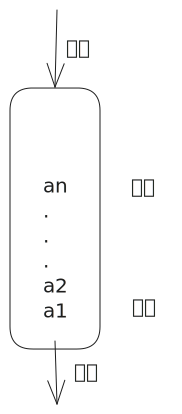
\includegraphics[width=0.2\textwidth]{./figure/pdf/cropped/seqQueue.pdf}
  \caption{顺序队列}
  \label{fig:seqQueue}
\end{figure}

顺序队列的结构体定义如代码\ref{lst:seqQueueStruct}所示。

\begin{lstlisting}[language=C++, caption={顺序队列结构体定义}, label={lst:seqQueueStruct}]
  struct SeqQueue {
    int* data;//队列的数据元素
    int front;//队头指针
    int rear;//队尾指针
    int capacity;//队列的容量
  };
\end{lstlisting}


顺序队列的存放过程如图\ref{fig:seqQueuePut}所示。

\begin{figure}[h]
  \centering
  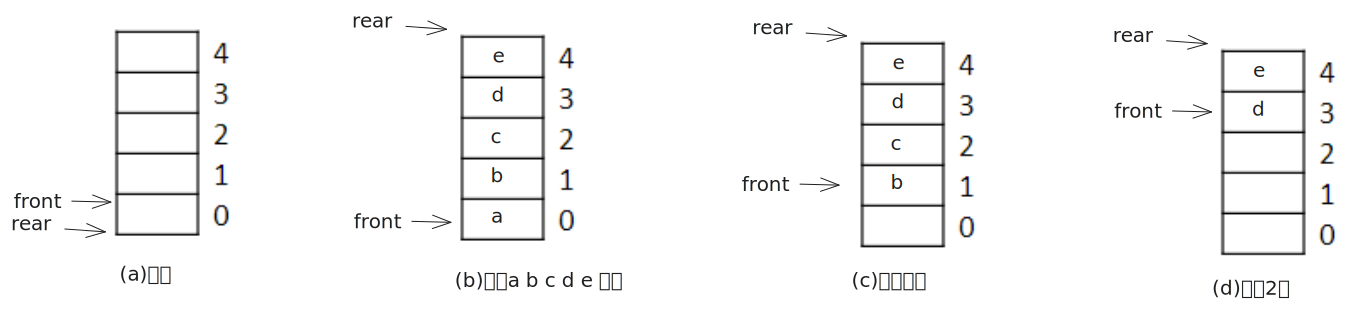
\includegraphics[width=1\textwidth]{./figure/pdf/cropped/seqQueuePut.pdf}
  \caption{顺序队列的存放过程}
  \label{fig:seqQueuePut}
\end{figure}

相关术语:

\begin{itemize}
  \item 队头指针:指向队头元素的前一个位置。
  \item 队尾指针:指向队尾元素。
  \item 队列的容量:队列的最大容量。
  \item 队列的大小:队列中包含的元素个数。
  \item 队列的长度:队列中包含的元素个数。
  \item 队列的空间:队列的容量减去队列的大小。
  \item 队列的空:队列的大小为0。
  \item 队列的满:队列的大小等于队列的容量。
\end{itemize}

顺序队列的基本操作包括创建、销毁、入队、出队、获取队头元素、判断队列是否为空、判断队列是否为满、获取队列的大小和获取队列的容量。

\textbf{创建操作}:

创建一个空顺序队列,需要为队列分配内存空间,并初始化队头指针、队尾指针和队列的容量。

代码如代码\ref{lst:createSeqQueue}所示。

\begin{lstlisting}[language=C++, caption={创建一个空顺序队列示例代码}, label={lst:createSeqQueue}]
  SeqQueue* createSeqQueue(int capacity) {
    SeqQueue* Q = (SeqQueue*)malloc(sizeof(SeqQueue));
    Q->data = (int*)malloc(sizeof(int) * capacity);
    Q->front = 0;
    Q->rear = 0;
    Q->capacity = capacity;
    return Q;
  }

\end{lstlisting}

该算法的总时间复杂度为 $O(1)$,空间复杂度为 $O(1)$。

特点:创建的顺序队列为空,不包含任何数据元素。

\textbf{销毁操作}:

销毁顺序队列,需要释放队列的内存空间。

代码如代码\ref{lst:destroySeqQueue}所示。

\begin{lstlisting}[language=C++, caption={销毁顺序队列示例代码}, label={lst:destroySeqQueue}]
  void destroySeqQueue(SeqQueue* Q) {
    free(Q->data);
    free(Q);
  }

\end{lstlisting}

该算法的总时间复杂度为 $O(1)$,空间复杂度为 $O(1)$。

特点:销毁顺序队列,释放队列的内存空间。

\textbf{判空操作}:

判断顺序队列是否为空,即队列中不包含任何元素。

代码如代码\ref{lst:isEmptySeqQueue}所示。

\begin{lstlisting}[language=C++, caption={判断顺序队列是否为空示例代码}, label={lst:isEmptySeqQueue}]
  bool isEmptySeqQueue(SeqQueue* Q) {
    return Q->front == Q->rear;
  }

\end{lstlisting}

该算法的总时间复杂度为 $O(1)$,空间复杂度为 $O(1)$。

特点:判断顺序队列是否为空,即队列中不包含任何元素。

\textbf{判满操作}:

判断顺序队列是否为满,即队列中包含的元素个数等于队列的容量。

代码如代码\ref{lst:isFullSeqQueue}所示。

\begin{lstlisting}[language=C++, caption={判断顺序队列是否为满示例代码}, label={lst:isFullSeqQueue}]
  bool isFullSeqQueue(SeqQueue* Q) {
    return (Q->rear + 1) % Q->capacity == Q->front;
  }

\end{lstlisting}

该算法的总时间复杂度为 $O(1)$,空间复杂度为 $O(1)$。

特点:判断顺序队列是否为满,即队列中包含的元素个数等于队列的容量。

\textbf{入队操作}:

将元素入队,即将元素放入队尾。

代码如代码\ref{lst:enQueueSeqQueue}所示。

\begin{lstlisting}[language=C++, caption={入队示例代码}, label={lst:enQueueSeqQueue}]
  void enQueueSeqQueue(SeqQueue* Q, int data) {
    if (isFullSeqQueue(Q)) {
      printf("队列已满,无法入队\n");
      return;
    }
    Q->data[Q->rear] = data;
    Q->rear = (Q->rear + 1) % Q->capacity;
  }

\end{lstlisting}

该算法的总时间复杂度为 $O(1)$,空间复杂度为 $O(1)$。

特点:将元素入队,即将元素放入队尾。

\textbf{出队操作}:

将元素出队,即将队头元素删除。

代码如代码\ref{lst:deQueueSeqQueue}所示。

\begin{lstlisting}[language=C++, caption={出队示例代码}, label={lst:deQueueSeqQueue}]
  void deQueueSeqQueue(SeqQueue* Q) {
    if (isEmptySeqQueue(Q)) {
      printf("队列为空,无法出队\n");
      return;
    }
    Q->front = (Q->front + 1) % Q->capacity;
  }

\end{lstlisting}

该算法的总时间复杂度为 $O(1)$,空间复杂度为 $O(1)$。

特点:将元素出队,即将队头元素删除。

\textbf{获取队头元素}:

获取顺序队列的队头元素,即获取队头元素的值。

代码如代码\ref{lst:getFrontSeqQueue}所示。

\begin{lstlisting}[language=C++, caption={获取队头元素示例代码}, label={lst:getFrontSeqQueue}]
  int getFrontSeqQueue(SeqQueue* Q) {
    if (isEmptySeqQueue(Q)) {
      printf("队列为空,无法获取队头元素\n");
      return -1;
    }
    return Q->data[Q->front];
  }

\end{lstlisting}

该算法的总时间复杂度为 $O(1)$,空间复杂度为 $O(1)$。

特点:获取顺序队列的队头元素,即获取队头元素的值。

\textbf{获取队列的大小}:

获取顺序队列的大小,即获取队列中包含的元素个数。

代码如代码\ref{lst:sizeSeqQueue}所示。

\begin{lstlisting}[language=C++, caption={获取队列的大小示例代码}, label={lst:sizeSeqQueue}]
  int sizeSeqQueue(SeqQueue* Q) {
    return (Q->rear - Q->front + Q->capacity) % Q->capacity;
  }

\end{lstlisting}

该算法的总时间复杂度为 $O(1)$,空间复杂度为 $O(1)$。

特点:获取顺序队列的大小,即获取队列中包含的元素个数。

\textbf{获取队列的容量}:

获取顺序队列的容量,即获取队列的最大容量。

代码如代码\ref{lst:capacitySeqQueue}所示。

\begin{lstlisting}[language=C++, caption={获取队列的容量示例代码}, label={lst:capacitySeqQueue}]
  int capacitySeqQueue(SeqQueue* Q) {
    return Q->capacity;
  }

\end{lstlisting}

该算法的总时间复杂度为 $O(1)$,空间复杂度为 $O(1)$。

特点:获取顺序队列的容量,即获取队列的最大容量。

\textbf{清空队列}:

清空顺序队列,即将队列中的所有元素删除。

代码如代码\ref{lst:clearSeqQueue}所示。

\begin{lstlisting}[language=C++, caption={清空队列示例代码}, label={lst:clearSeqQueue}]
  void clearSeqQueue(SeqQueue* Q) {
    Q->front = 0;
    Q->rear = 0;
  }

\end{lstlisting}

该算法的总时间复杂度为 $O(1)$,空间复杂度为 $O(1)$。

特点:清空顺序队列,即将队列中的所有元素删除。

\textbf{遍历队列}:

遍历顺序队列,即输出队列中的所有元素。

代码如代码\ref{lst:traverseSeqQueue}所示。

\begin{lstlisting}[language=C++, caption={遍历队列示例代码}, label={lst:traverseSeqQueue}]
  void traverseSeqQueue(SeqQueue* Q) {
    for (int i = Q->front; i != Q->rear; i = (i + 1) % Q->capacity) {
      printf("%d ", Q->data[i]);
    }
    printf("\n");
  }

\end{lstlisting}

该算法的总时间复杂度为 $O(n)$,空间复杂度为 $O(1)$。

特点:遍历顺序队列,即输出队列中的所有元素。

针对循环队列,我们还可以使用另外两种方法来判断队列是否为空和队列是否为满。

第一种:使用一个变量记录队列的大小,当队列为空时,队列的大小为0;当队列为满时,队列的大小等于队列的容量。

第二种:新增一个tag变量,当队列为空时,tag等于0;当队列为满时,tag等于1。
第一种的结构体为:

\begin{lstlisting}[language=C++, caption={循环队列结构体定义}, label={lst:circleQueueStruct}]
  struct CircleQueue {
    int* data;//队列的数据元素
    int front;//队头指针
    int rear;//队尾指针
    int size;//队列的大小
    int capacity;//队列的容量
  };
\end{lstlisting}

\textbf{判空操作}:

判断循环队列是否为空,即队列中不包含任何元素。

代码如代码\ref{lst:isEmptyCircleQueue}所示。

\begin{lstlisting}[language=C++, caption={判断循环队列是否为空示例代码}, label={lst:isEmptyCircleQueue}]
  bool isEmptyCircleQueue(CircleQueue* Q) {
    return Q->size == 0;
  }

\end{lstlisting}

\textbf{判满操作}:

判断循环队列是否为满,即队列中包含的元素个数等于队列的容量。

代码如代码\ref{lst:isFullCircleQueue}所示。

\begin{lstlisting}[language=C++, caption={判断循环队列是否为满示例代码}, label={lst:isFullCircleQueue}]
  bool isFullCircleQueue(CircleQueue* Q) {
    return Q->size == Q->capacity;
  }

\end{lstlisting}

第二种的结构体为:

\begin{lstlisting}[language=C++, caption={循环队列结构体定义}, label={lst:circleQueueStruct}]
  struct CircleQueue {
    int* data;//队列的数据元素
    int front;//队头指针
    int rear;//队尾指针
    int tag;//标记队列是否为满
    int capacity;//队列的容量
  };
\end{lstlisting}

\textbf{判空操作}:

判断循环队列是否为空,即队列中不包含任何元素。

代码如代码\ref{lst:isEmptyCircleQueue}所示。

\begin{lstlisting}[language=C++, caption={判断循环队列是否为空示例代码}, label={lst:isEmptyCircleQueue}]
  bool isEmptyCircleQueue(CircleQueue* Q) {
    return Q->front == Q->rear && Q->tag == 0;
  }

\end{lstlisting}

\textbf{判满操作}:

判断循环队列是否为满,即队列中包含的元素个数等于队列的容量。

代码如代码\ref{lst:isFullCircleQueue}所示。

\begin{lstlisting}[language=C++, caption={判断循环队列是否为满示例代码}, label={lst:isFullCircleQueue}]
  bool isFullCircleQueue(CircleQueue* Q) {
    return Q->front == Q->rear && Q->tag == 1;
  }

\end{lstlisting}

\subsection{链式队列}

链式队列是使用链表实现的队列,队列的大小是动态的,队列的容量是无限的。

链式队列的结构如如图\ref{fig:linkQueue}所示。

\begin{figure}[h]
  \centering
  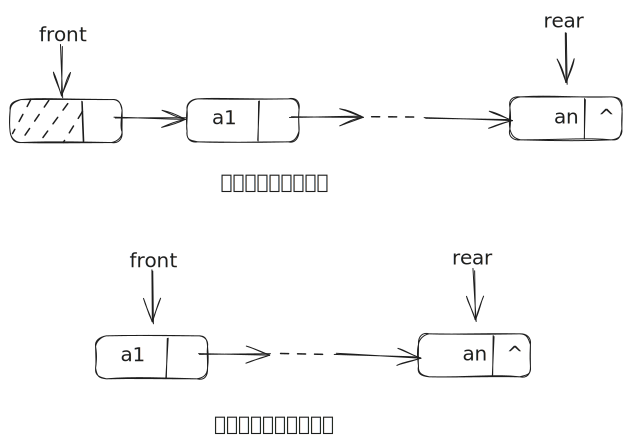
\includegraphics[width=1\textwidth]{./figure/pdf/cropped/linkQueue.pdf}
  \caption{链式队列}
  \label{fig:linkQueue}
\end{figure}

图中示出了两类链式队列,一类带头结点,一类不带头结点。

我们可以发现,不带头结点的链式队列需要特殊处理队列为空的情况,因为队列为空时,
队头指针和队尾指针都为空。因此,我们通常使用带头结点的链式队列。

链式队列的结构体定义如代码\ref{lst:linkQueueStruct}所示。

\begin{lstlisting}[language=C++, caption={链式队列结构体定义}, label={lst:linkQueueStruct}]
  struct singleLink {
	NODETYPE data;
	singleLink* next;
  }; 
  struct LinkQueue {
    singleLink* front, * rear;
  };
\end{lstlisting}

链式队列的基本操作包括创建、销毁、入队、出队、获取队头元素、判断队列是否为空、获取队列的大小。

\textbf{创建操作}:

创建一个空链式队列,需要为队列分配内存空间,并初始化队头指针和队尾指针。

代码如代码\ref{lst:createLinkQueue}所示。

\begin{lstlisting}[language=C++, caption={创建一个空链式队列示例代码}, label={lst:createLinkQueue}]
  LinkQueue* createLinkQueue() {
    singleLink* h = (singleLink*)malloc(sizeof(singleLink));
    LinkQueue* Q = (LinkQueue*)malloc(sizeof(LinkQueue));
    Q->front = h;
    Q->rear = h;
    return Q;
  }

该算法的总时间复杂度为 $O(1)$,空间复杂度为 $O(1)$。

特点:创建的链式队列为空,不包含任何数据元素。

\textbf{销毁操作}:

销毁链式队列,需要释放队列的内存空间。

代码如代码\ref{lst:destroyLinkQueue}所示。

\begin{lstlisting}[language=C++, caption={销毁链式队列示例代码}, label={lst:destroyLinkQueue}]
  void destroyLinkQueue(LinkQueue* Q) {
    singleLink* p = Q->front;
    while (p != NULL) {
      singleLink* q = p;
      p = p->next;
      free(q);
    }
    free(Q);
  }

\end{lstlisting}

该算法的总时间复杂度为 $O(n)$,空间复杂度为 $O(1)$。

特点:销毁链式队列,释放队列的内存空间。

\textbf{判空操作}:

判断链式队列是否为空,即队列中不包含任何元素。

代码如代码\ref{lst:isEmptyLinkQueue}所示。

\begin{lstlisting}[language=C++, caption={判断链式队列是否为空示例代码}, label={lst:isEmptyLinkQueue}]
  bool isEmptyLinkQueue(LinkQueue* Q) {
    return Q->front == Q->rear;
  }

\end{lstlisting}

该算法的总时间复杂度为 $O(1)$,空间复杂度为 $O(1)$。

特点:判断链式队列是否为空,即队列中不包含任何元素。

\textbf{入队操作}:

将元素入队,即将元素放入队尾。

代码如代码\ref{lst:enQueueLinkQueue}所示。

\begin{lstlisting}[language=C++, caption={入队示例代码}, label={lst:enQueueLinkQueue}]
  void enQueueLinkQueue(LinkQueue* Q, NODETYPE data) {
    singleLink* p = (singleLink*)malloc(sizeof(singleLink));
    p->data = data;
    p->next = NULL;
    Q->rear->next = p;
    Q->rear = p;
  }

\end{lstlisting}

该算法的总时间复杂度为 $O(1)$,空间复杂度为 $O(1)$。

特点:将元素入队,即将元素放入队尾。

\textbf{出队操作}:

将元素出队,即将队头元素删除。

代码如代码\ref{lst:deQueueLinkQueue}所示。

\begin{lstlisting}[language=C++, caption={出队示例代码}, label={lst:deQueueLinkQueue}]
  void deQueueLinkQueue(LinkQueue* Q) {
    if (isEmptyLinkQueue(Q)) {
      printf("队列为空,无法出队\n");
      return;
    }
    singleLink* p = Q->front->next;
    Q->front->next = p->next;
    if (Q->rear == p) {
      Q->rear = Q->front;
    }
    free(p);
  }

\end{lstlisting}

该算法的总时间复杂度为 $O(1)$,空间复杂度为 $O(1)$。

特点:将元素出队,即将队头元素删除。

\textbf{获取队头元素}:

获取链式队列的队头元素,即获取队头元素的值。

代码如代码\ref{lst:getFrontLinkQueue}所示。

\begin{lstlisting}[language=C++, caption={获取队头元素示例代码}, label={lst:getFrontLinkQueue}]
  NODETYPE getFrontLinkQueue(LinkQueue* Q) {
    if (isEmptyLinkQueue(Q)) {
      printf("队列为空,无法获取队头元素\n");
      return -1;
    }
    return Q->front->next->data;
  }

\end{lstlisting}

该算法的总时间复杂度为 $O(1)$,空间复杂度为 $O(1)$。

特点:获取链式队列的队头元素,即获取队头元素的值。

\textbf{获取队列的大小}:

获取链式队列的大小,即获取队列中包含的元素个数。

代码如代码\ref{lst:sizeLinkQueue}所示。

\begin{lstlisting}[language=C++, caption={获取队列的大小示例代码}, label={lst:sizeLinkQueue}]
  int sizeLinkQueue(LinkQueue* Q) {
    int size = 0;
    singleLink* p = Q->front->next;
    while (p != NULL) {
      size++;
      p = p->next;
    }
    return size;
  }

\end{lstlisting}

该算法的总时间复杂度为 $O(n)$,空间复杂度为 $O(1)$。

特点:获取链式队列的大小,即获取队列中包含的元素个数。

\textbf{清空队列}:

清空链式队列,即将队列中的所有元素删除。

代码如代码\ref{lst:clearLinkQueue}所示。

\begin{lstlisting}[language=C++, caption={清空队列示例代码}, label={lst:clearLinkQueue}]
  void clearLinkQueue(LinkQueue* Q) {
    singleLink* p = Q->front->next;
    while (p != NULL) {
      singleLink* q = p;
      p = p->next;
      free(q);
    }
    Q->rear = Q->front;
  }

\end{lstlisting}

该算法的总时间复杂度为 $O(n)$,空间复杂度为 $O(1)$。

特点:清空链式队列,即将队列中的所有元素删除。

\textbf{遍历队列}:

遍历链式队列,即输出队列中的所有元素。

代码如代码\ref{lst:traverseLinkQueue}所示。

\begin{lstlisting}[language=C++, caption={遍历队列示例代码}, label={lst:traverseLinkQueue}]
  void traverseLinkQueue(LinkQueue* Q) {
    singleLink* p = Q->front->next;
    while (p != NULL) {
      printf("%d ", p->data);
      p = p->next;
    }
    printf("\n");
  }

\end{lstlisting}

该算法的总时间复杂度为 $O(n)$,空间复杂度为 $O(1)$。

特点:遍历链式队列,即输出队列中的所有元素。





\subsection{双端队列}

双端队列是一种具有队列和栈的性质的线性表,双端队列的两端都可以进行插入和删除操作。

双端队列的结构如如图\ref{fig:deque}所示。

\begin{figure}[h]
  \centering
  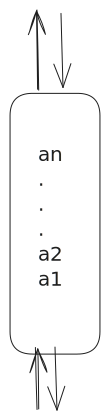
\includegraphics[width=0.1\textwidth]{./figure/pdf/cropped/DQueue.pdf}
  \caption{双端队列}
  \label{fig:deque}
\end{figure}


\section{栈和队列的应用}

\subsection{栈的应用}

\subsubsection{简单表达式求值}

这里限定的简单表达式是用户输入的一个包含+、-、*、/、(、)和正整数的合法算数表达式,计算该表达式的运算结果。

在算术表达式中, 运算符位于两个操作数中间的表达式称为中缀表达式 (infix
expression) ,例如 1十2* 3 就是一个中绥表达式。中组表达式是一种最常用的表达式形式,
日常生活中的表达式一般都是中绥表达式。

对中组表达式的运算一般遵循“先乘除,后加减,从左到右计算,先括号内,后括号外?的
规则,因此中组表达式不仅要依赖运算符优先级,还要处理括号。

算术表达式的另一种形式是后缀表达式(postfix expression)或逆波兰表达式,就是在
算术表达式中运算符在操作数的后面,如1+2* 3 的后组表达式为12 3 * +。在后缀表
达式中已经考虑了运算符的优先级,没有括号,只有操作数和运算符,而且越放在前面的运
算符越优先执行。

同样,在算术表达式中,如果运算符在操作数的前面,称为前缀表达式 (prefix
expression) ,如 1+2* 3 的前缀表达式为+1 * 2 3。

后缀表达式是一种十分有用的表达式,它将复杂表达式转换为可以依靠简单的操作得
到计算结果的表达式。所以对中绥表达式的求值过程是先将中绥算术表达式转换成后缀表
达式,然后对该后缀表达式求值。


\textbf{中缀表达式转后缀表达式}

中缀表达式转后缀表达式的算法如下:

1. 从左到右扫描中缀表达式。

2. 如果是操作数,则直接输出。

3. 如果是运算符,则判断其与栈顶运算符的优先级,是右括号或优先级低于栈顶运算符,则栈顶运算符依次出栈并输出,直到遇到左括号或栈空为止。此时将当前运算符入栈。

4. 如果是左括号,则直接入栈。

5. 如果是右括号,则依次出栈并输出直到遇到左括号,左括号出栈。

6. 重复2-5步骤,直到表达式的最右端。

7. 将栈中的运算符依次出栈并输出。

例如,中缀表达式$3+5*8-(6 + 2)$转换为后缀表达式的过程如表\ref{tab:infixToPostfix}所示。


\begin{table}[h!]
  \centering
  \begin{tabular}{|c|c|c|}
  \hline
  \textbf{扫描的符号} & \textbf{栈 (Stack)} & \textbf{输出 (Output)} \\ \hline
  3 &  & 3 \\ \hline
  + & + & 3 \\ \hline
  5 & + & 3 5 \\ \hline
  * & + * & 3 5 \\ \hline
  8 & + * & 3 5 8 \\ \hline
  - & - & 3 5 8 * + \\ \hline
  ( & - ( & 3 5 8 * + \\ \hline
  6 & - ( & 3 5 8 * + 6 \\ \hline
  + & - ( + & 3 5 8 * + 6 \\ \hline
  2 & - ( + & 3 5 8 * + 6 2 \\ \hline
  ) & - & 3 5 8 * + 6 2 + \\ \hline
  (结束) &  & 3 5 8 * + 6 2 + - \\ \hline
  \end{tabular}
  \caption{前缀转后缀}
  \label{tab:infixToPostfix}
  \end{table}

代码如代码\ref{lst:infixToPostfix}所示。

\begin{lstlisting}[language=C++, caption={中缀表达式转后缀表达式示例代码}, label={lst:infixToPostfix}]
  bool isOperator(char c) {
    return c == '+' || c == '-' || c == '*' || c == '/';
  }

  int priority(char c) {
    if (c == '+' || c == '-') {
      return 1;
    }
    if (c == '*' || c == '/') {
      return 2;
    }
    return 0;
  }

  string infixToPostfix(string infix) {
    stack<char> s;
    string postfix = "";
    for (int i = 0; i < infix.size(); i++) {
      if (isdigit(infix[i])) {
        postfix += infix[i];
      } else if (infix[i] == '(') {
        s.push(infix[i]);
      } else if (infix[i] == ')') {
        while (!s.empty() && s.top() != '(') {
          postfix += s.top();
          s.pop();
        }
        s.pop();
      } else if (isOperator(infix[i])) {
        while (!s.empty() && priority(s.top()) >= priority(infix[i])) {
          postfix += s.top();
          s.pop();
        }
        s.push(infix[i]);
      }
    }
    while (!s.empty()) {
      postfix += s.top();
      s.pop();
    }
    return postfix;
  }

\end{lstlisting}

该算法的总时间复杂度为 $O(n)$,空间复杂度为 $O(n)$。

特点:中缀表达式转后缀表达式。

\textbf{后缀表达式求值}

后缀表达式求值的算法如下:

1. 从左到右扫描后缀表达式。

2. 如果是操作数,则入栈。

3. 如果是运算符,则从栈中弹出两个操作数,进行运算,将运算结果入栈。

4. 重复2-3步骤,直到表达式的最右端。

5. 栈中的元素即为表达式的运算结果。

例如,后缀表达式$3 5 8 * + 6 2 + -$的求值过程如表\ref{tab:postfixEvaluation}所示。

\begin{table}[h!]
  \centering
  \begin{tabular}{|c|c|}
  \hline
  \textbf{扫描的符号} & \textbf{栈 (Stack)} \\ \hline
  3 & 3 \\ \hline
  5 & 3 5 \\ \hline
  8 & 3 5 8 \\ \hline
  * & 3 40 \\ \hline
  + & 43 \\ \hline
  6 & 43 6 \\ \hline
  2 & 43 6 2 \\ \hline
  + & 43 8 \\ \hline
  - & 35 \\ \hline
  \end{tabular}
  \caption{后缀表达式求值}
  \label{tab:postfixEvaluation}
  \end{table}

代码如代码\ref{lst:postfixEvaluation}所示。

\begin{lstlisting}[language=C++, caption={后缀表达式求值示例代码}, label={lst:postfixEvaluation}]
  int postfixEvaluation(string postfix) {
    stack<int> s;
    for (int i = 0; i < postfix.size(); i++) {
      if (isdigit(postfix[i])) {
        s.push(postfix[i] - '0');
      } else {
        int b = s.top();
        s.pop();
        int a = s.top();
        s.pop();
        if (postfix[i] == '+') {
          s.push(a + b);
        } else if (postfix[i] == '-') {
          s.push(a - b);
        } else if (postfix[i] == '*') {
          s.push(a * b);
        } else if (postfix[i] == '/') {
          s.push(a / b);
        }
      }
    }
    return s.top();
  }

\end{lstlisting}


\subsubsection{括号匹配}

括号匹配是指对于一个字符串,其中包含的括号必须是成对出现的,且左括号必须在右括号的前面。

例如,字符串“((()))”是括号匹配的,而字符串“(()))”不是括号匹配的。

括号匹配的算法如下:

1. 从左到右扫描字符串。

2. 如果是左括号,则入栈。

3. 如果是右括号,则判断栈是否为空,如果为空,则返回false;否则,出栈。

4. 重复2-3步骤,直到字符串的最右端。

5. 如果栈为空,则返回true;否则,返回false。

例如,字符串“(())()”的括号匹配过程如表\ref{tab:bracketMatching}所示。

\begin{table}[h!]
  \centering
  \begin{tabular}{|c|c|c|}
  \hline
  \textbf{扫描的符号} & \textbf{栈 (Stack)} & \textbf{是否匹配} \\ \hline
  ( & ( &  \\ \hline
  ( & (( &  \\ \hline
  ) & ( &  \\ \hline
  ) &  &  \\ \hline
  ( & ( &  \\ \hline
  ) &  &  \\ \hline
  (结束) &  & 是 \\ \hline
  \end{tabular}
  \caption{括号匹配}
  \label{tab:bracketMatching}
  \end{table}

代码如代码\ref{lst:bracketMatching}所示。

\begin{lstlisting}[language=C++, caption={括号匹配示例代码}, label={lst:bracketMatching}]
  bool bracketMatching(string s) {
    stack<char> st;
    for (int i = 0; i < s.size(); i++) {
      if (s[i] == '(') {
        st.push(s[i]);
      } else if (s[i] == ')') {
        if (st.empty()) {
          return false;
        }
        st.pop();
      }
    }
    return st.empty();
  }

\end{lstlisting}

该算法的总时间复杂度为 $O(n)$,空间复杂度为 $O(n)$。

特点:括号匹配。

\subsection{队列的应用}

\subsubsection{约瑟夫环问题}

约瑟夫环问题是一个著名的问题,是一个数学的应用问题,该问题的大致描述如下:

设有n个人围成一圈,从第一个人开始报数,报到m的人出列,然后从出列的下一个人开始重新报数,报到m的人出列,如此循环,直到所有的人都出列为止。

例如,当n=6,m=5时,出列的顺序为5、4、6、2、3、1。

约瑟夫环问题的算法如下:

1. 创建一个队列,将所有的人依次入队。

2. 从队头开始,依次出队,报数,如果报数为m,则出队;否则,重新入队。

3. 重复2步骤,直到队列为空。

例如,当n=6,m=5时,出列的顺序为5、4、6、2、3、1。

代码如代码\ref{lst:josephus}所示。

\begin{lstlisting}[language=C++, caption={约瑟夫环问题示例代码}, label={lst:josephus}]
  void josephus(int n, int m) {
    queue<int> q;
    for (int i = 1; i <= n; i++) {
      q.push(i);
    }
    while (!q.empty()) {
      for (int i = 1; i < m; i++) {
        q.push(q.front());
        q.pop();
      }
      cout << q.front() << " ";
      q.pop();
    }
  }

\end{lstlisting}

该算法的总时间复杂度为 $O(nm)$,空间复杂度为 $O(n)$。

特点:约瑟夫环问题。




\chapter{串}

串(string)是由零个或多个字符组成的有限序列。含零个字符的串称为空串,用多表
示。串中所含字符的个数称为该串的长度(或串长)。通常将一个串表示成"aa …a, 的形
式,其中最外边的双引号(或单引号)不是串的内容,它们是串的标志,用于将串与标识符(如
变量名等)加以区别。每个 w(1委未站代表一个字符,不同的机器和编程语言对合法字符
〈即人允许使用的字符)有不同的规定。但在一般情况下,英文字母.数字(0,1,…,9)和常用的
标点符号以及空格符等都是合法的字符。

两个串相等当且仅当这两个串的长度相等并且各对应位置上的字符都
相同。一个串中任意个连续字符组成的序列称为该串的子串(substring),
例如串"abcde"的子串有"a"、ab"、abc"和"abcd"等。为了表述清楚,在串
中空格字符用“0D"”符号表示,例如"aDOb"是一个长度为4的串,其中含有两
个空格字符。空串是不包含任何字符的串,其长度为 0,空串是任何串的
子串


\section{串的存储结构}

串的存储结构有两种,即顺序存储结构和链式存储结构。
\subsection{顺序存储结构}


顺序串中的字符被依次存放在一组连续的存储单元里。一般来说,一个字节(8 位)可
以表示一个字符(存放其 ASCII 码) 。而计算机内存是按字编址的,即以字为存储单位,一
个存储单元指的是一个字。而一个字可能包含多个字节,其所包含的字节数随机器而异。

顺序串的存储方式有两种: 一种是每个字只存一个字符,如图\ref{fig:seqString}所示(假设一个字包
含4个字节) ,这称为非紧缩格式(其存储密度小); 另一种是每个字存放多个字符,如图\ref{fig:tightSeqString}
所示 ,这称为紧缩格式(其存储密度大) 。在这两个图中,有阴影的字节为空闲部分。



\begin{figure}[h]
  \centering
  \includegraphics[width=0.2\textwidth]{./figure/pdf/cropped/narrowString.pdf}
  \caption{非紧缩格式的顺序串}
  \label{fig:seqString}
\end{figure}


\begin{figure}[h]
  \centering
  \includegraphics[width=0.2\textwidth]{./figure/pdf/cropped/notNarrowString.pdf}
  \caption{紧缩格式的顺序串}
  \label{fig:tightSeqString}
\end{figure}

串的紧缩格式存储方式是将串中的字符紧凑地存放在存储单元中,这样可以节省存储空间。
但是,在插入和删除操作时,需要移动大量的字符,因此效率较低。非紧缩格式存储方式是将 串中的字符依次存放在存储单元中,字符之间不留空,这样可以方便地进行插入和删除操作。
但是,由于字符之间没有留空,因此存储密度较低。
我们主要讨论非紧缩格式的顺序串。

顺序串的结构如代码\ref{lst:seqStringStruct}所示。

\begin{lstlisting}[language=C++, caption={顺序串结构体定义}, label={lst:seqStringStruct}]
  struct SeqString {
    char data[MAXSIZE];//存放串的字符数组
    int length;//串的长度
  };
\end{lstlisting}

顺序串的基本操作包括创建、销毁、清空、获取长度、获取字符、连接、比较、插入、删除、替换、复制、判断相等、求子串、输出等。

\textbf{创建操作}:

创建一个空串,需要为串分配内存空间,并初始化串的长度。

代码如代码\ref{lst:createSeqString}所示。

\begin{lstlisting}[language=C++, caption={创建一个空串示例代码}, label={lst:createSeqString}]
  SeqString* createSeqString() {
    SeqString* s = (SeqString*)malloc(sizeof(SeqString));
    s->length = 0;
    return s;
  }

\end{lstlisting}

该算法的总时间复杂度为 $O(1)$,空间复杂度为 $O(1)$。

特点:创建一个空串。

\textbf{销毁操作}:

销毁串,需要释放串的内存空间。

代码如代码\ref{lst:destroySeqString}所示。

\begin{lstlisting}[language=C++, caption={销毁串示例代码}, label={lst:destroySeqString}]
  void destroySeqString(SeqString* s) {
    free(s);
  }

\end{lstlisting}

该算法的总时间复杂度为 $O(1)$,空间复杂度为 $O(1)$。

特点:销毁串。

\textbf{清空操作}:

清空串,即将串的长度设置为0。

代码如代码\ref{lst:clearSeqString}所示。

\begin{lstlisting}[language=C++, caption={清空串示例代码}, label={lst:clearSeqString}]
  void clearSeqString(SeqString* s) {
    s->length = 0;
  }

\end{lstlisting}

该算法的总时间复杂度为 $O(1)$,空间复杂度为 $O(1)$。

特点:清空串。

\textbf{获取长度操作}:

获取串的长度。

代码如代码\ref{lst:lengthSeqString}所示。

\begin{lstlisting}[language=C++, caption={获取串的长度示例代码}, label={lst:lengthSeqString}]
  int lengthSeqString(SeqString* s) {
    return s->length;
  }

\end{lstlisting}

该算法的总时间复杂度为 $O(1)$,空间复杂度为 $O(1)$。

特点:获取串的长度。

\textbf{获取字符操作}:

获取串中指定位置的字符。

代码如代码\ref{lst:getSeqString}所示。

\begin{lstlisting}[language=C++, caption={获取串中指定位置的字符示例代码}, label={lst:getSeqString}]
  char getSeqString(SeqString* s, int i) {
    if (i < 0 || i >= s->length) {
      printf("位置不合法\n");
      return -1;
    }
    return s->data[i];
  }

\end{lstlisting}

该算法的总时间复杂度为 $O(1)$,空间复杂度为 $O(1)$。

特点:获取串中指定位置的字符。

\textbf{连接操作}:

连接两个串,即将两个串连接成一个串。

代码如代码\ref{lst:concatSeqString}所示。

\begin{lstlisting}[language=C++, caption={连接两个串示例代码}, label={lst:concatSeqString}]
  SeqString* concatSeqString(SeqString* s1, SeqString* s2) {
    SeqString* s = createSeqString();
    for (int i = 0; i < s1->length; i++) {
      s->data[s->length++] = s1->data[i];
    }
    for (int i = 0; i < s2->length; i++) {
      s->data[s->length++] = s2->data[i];
    }
    return s;
  }

\end{lstlisting}

该算法的总时间复杂度为 $O(n)$,空间复杂度为 $O(n)$。

特点:连接两个串。

\textbf{比较操作}:

比较两个串的大小。

代码如代码\ref{lst:compareSeqString}所示。

\begin{lstlisting}[language=C++, caption={比较两个串的大小示例代码}, label={lst:compareSeqString}]
  int compareSeqString(SeqString* s1, SeqString* s2) {//s1>s2返回正数,s1=s2返回0,s1<s2返回负数
    int i = 0;
    while (i < s1->length && i < s2->length) {//比较两个串的公共部分
      if (s1->data[i] != s2->data[i]) {//如果两个串的字符不相等
        return s1->data[i] - s2->data[i];
      }
      i++;
    }
    return s1->length - s2->length;
  }

\end{lstlisting}

该算法的总时间复杂度为 $O(n)$,空间复杂度为 $O(1)$。

特点:比较两个串的大小。

\textbf{插入操作}:

在指定位置插入子串。

代码如代码\ref{lst:insertSeqString}所示。

\begin{lstlisting}[language=C++, caption={在指定位置插入子串示例代码}, label={lst:insertSeqString}]
  void insertSeqString(SeqString* s, int i, SeqString* t) {
    if (i < 0 || i > s->length) {
      printf("位置不合法\n");
      return;
    }
    for (int j = s->length - 1; j >= i; j--) {//将i位置及其后面的字符后移
      s->data[j + t->length] = s->data[j];
    }
    for (int j = 0; j < t->length; j++) {//将t中的字符插入到i位置
      s->data[i + j] = t->data[j];
    }
    s->length += t->length;//修改串的长度
  }

\end{lstlisting}

该算法的总时间复杂度为 $O(n)$,空间复杂度为 $O(1)$。

特点:在指定位置插入子串。

\textbf{删除操作}:

删除指定位置的子串。

代码如代码\ref{lst:deleteSeqString}所示。

\begin{lstlisting}[language=C++, caption={删除指定位置的子串示例代码}, label={lst:deleteSeqString}]
  void deleteSeqString(SeqString* s, int i, int len) {
    if (i < 0 || i >= s->length || len < 0 || i + len > s->length) {
      printf("位置不合法\n");
      return;
    }
    for (int j = i + len; j < s->length; j++) {//将i+len位置及其后面的字符前移
      s->data[j - len] = s->data[j];
    }
    s->length -= len;//修改串的长度
  }

\end{lstlisting}

该算法的总时间复杂度为 $O(n)$,空间复杂度为 $O(1)$。

特点:删除指定位置的子串。

\textbf{替换操作}:

替换指定位置的子串。

代码如代码\ref{lst:replaceSeqString}所示。

\begin{lstlisting}[language=C++, caption={替换指定位置的子串示例代码}, label={lst:replaceSeqString}]
  void replaceSeqString(SeqString* s, int i, int len, SeqString* t) {
    if (i < 0 || i >= s->length || len < 0 || i + len > s->length) {
      printf("位置不合法\n");
      return;
    }
    for (int j = i + len; j < s->length; j++) {//将i+len位置及其后面的字符前移
      s->data[j - len + t->length] = s->data[j];
    }
    for (int j = 0; j < t->length; j++) {//将t中的字符插入到i位置
      s->data[i + j] = t->data[j];
    }
    s->length = s->length - len + t->length;//修改串的长度
  }

\end{lstlisting}

该算法的总时间复杂度为 $O(n)$,空间复杂度为 $O(1)$。

特点:替换指定位置的子串。

\textbf{复制操作}:

复制串。

代码如代码\ref{lst:copySeqString}所示。

\begin{lstlisting}[language=C++, caption={复制串示例代码}, label={lst:copySeqString}]
  SeqString* copySeqString(SeqString* s) {
    SeqString* t = createSeqString();
    for (int i = 0; i < s->length; i++) {
      t->data[i] = s->data[i];
    }
    t->length = s->length;
    return t;
  }

\end{lstlisting}

该算法的总时间复杂度为 $O(n)$,空间复杂度为 $O(n)$。

特点:复制串。

\textbf{判断相等操作}:

判断两个串是否相等。

代码如代码\ref{lst:equalSeqString}所示。

\begin{lstlisting}[language=C++, caption={判断两个串是否相等示例代码}, label={lst:equalSeqString}]
  bool equalSeqString(SeqString* s1, SeqString* s2) {
    if (s1->length != s2->length) {
      return false;
    }
    for (int i = 0; i < s1->length; i++) {
      if (s1->data[i] != s2->data[i]) {
        return false;
      }
    }
    return true;
  }

\end{lstlisting}

该算法的总时间复杂度为 $O(n)$,空间复杂度为 $O(1)$。

特点:判断两个串是否相等。

\textbf{求子串操作}:

求串的子串。

代码如代码\ref{lst:subSeqString}所示。

\begin{lstlisting}[language=C++, caption={求串的子串示例代码}, label={lst:subSeqString}]
  SeqString* subSeqString(SeqString* s, int i, int len) {
    if (i < 0 || i >= s->length || len < 0 || i + len > s->length) {
      printf("位置不合法\n");
      return NULL;
    }
    SeqString* t = createSeqString();
    for (int j = 0; j < len; j++) {
      t->data[j] = s->data[i + j];
    }
    t->length = len;
    return t;
  }

\end{lstlisting}

该算法的总时间复杂度为 $O(n)$,空间复杂度为 $O(n)$。

特点:求串的子串。

\textbf{输出操作}:

输出串。

代码如代码\ref{lst:printSeqString}所示。

\begin{lstlisting}[language=C++, caption={输出串示例代码}, label={lst:printSeqString}]
  void printSeqString(SeqString* s) {
    for (int i = 0; i < s->length; i++) {
      printf("%c", s->data[i]);
    }
    printf("\n");
  }

\end{lstlisting}

该算法的总时间复杂度为 $O(n)$,空间复杂度为 $O(1)$。

特点:输出串。


\subsection{链式存储结构}

串采用链式存储结构存储时称为链串,这里采用带头结点的单链表作为链串。链串的
组织形式与一般的单链表类似,主要区别在于链串中的一个结点可以存储多个字符。通常
将链串中每个结点所存储的字符个数称为结点大小。图\ref{fig:linkStr_fourNodes}和图 \ref{fig:linkStr_oneNode}分别表示同一个串
"ABCDEFGHIJKLMN "的结点大小为 4(存储密度大)和 1(存储密度小)时的链串结构 。


\begin{figure}[h]
  \centering
  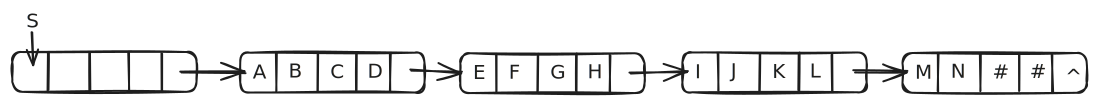
\includegraphics[width=0.8\textwidth]{./figure/pdf/cropped/linkStr_fourNodes.pdf}
  \caption{结点大小为4的链串}
  \label{fig:linkStr_fourNodes}

\end{figure}

\begin{figure}[h]
  \centering
  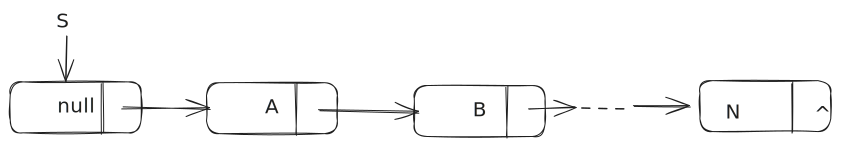
\includegraphics[width=0.6\textwidth]{./figure/pdf/cropped/linkStr_oneNode.pdf}
  \caption{结点大小为1的链串}
  \label{fig:linkStr_oneNode}

\end{figure}

当绪点大小大于 1(例如结点大小为4)时,链串的尾结点的各个数据域不一定总能全被
字符占满,此时应在这些未占用的数据域里补上不属于字符集的特殊符号(例如' \# '字符),
以示区别(参见图\ref{fig:linkStr_fourNodes} 中的尾结点) 。

在链串中 ,结点大小越大,存储密度越大,但一些基本操作(如插入、删除、替换等)有所
不便,且可能引起大量字符移动,因此它适合于串很少修改的情况; 结点大小越小(如结点
大小为 1 时) ,相关操作的实现越方便,但存储密度下降。为简便起见,这里规定链串结点大
小均为1。

链串的结构如代码\ref{lst:linkStringStruct}所示。

\begin{lstlisting}[language=C++, caption={链串结构体定义}, label={lst:linkStringStruct}]
  struct LinkNode {
    char data;//存放字符
    LinkNode* next;//指向下一个结点
  };

  struct LinkString {
    LinkNode* head;//头结点
    int length;//串的长度
  };
\end{lstlisting}

\section{串的操作}

串的操作包括创建、销毁、清空、获取长度、获取字符、连接、比较、插入、删除、替换、复制、判断相等、求子串、输出等。

\textbf{创建操作}:

创建一个空串,需要为串分配内存空间,并初始化串的长度。

代码如代码\ref{lst:createLinkString}所示。

\begin{lstlisting}[language=C++, caption={创建一个空串示例代码}, label={lst:createLinkString}]
  LinkString* createLinkString() {
    LinkString* s = (LinkString*)malloc(sizeof(LinkString));
    s->head = NULL;
    s->length = 0;
    return s;
  }

\end{lstlisting}

该算法的总时间复杂度为 $O(1)$,空间复杂度为 $O(1)$。

特点:创建一个空串。

\textbf{销毁操作}:

销毁串,需要释放串的内存空间。

代码如代码\ref{lst:destroyLinkString}所示。

\begin{lstlisting}[language=C++, caption={销毁串示例代码}, label={lst:destroyLinkString}]
  void destroyLinkString(LinkString* s) {
    LinkNode* p = s->head;
    while (p != NULL) {
      LinkNode* q = p;
      p = p->next;
      free(q);
    }
    free(s);
  }

\end{lstlisting}

该算法的总时间复杂度为 $O(n)$,空间复杂度为 $O(1)$。

特点:销毁串。

\textbf{清空操作}:

清空串,即将串的长度设置为0。

代码如代码\ref{lst:clearLinkString}所示。

\begin{lstlisting}[language=C++, caption={清空串示例代码}, label={lst:clearLinkString}]
  void clearLinkString(LinkString* s) {
    LinkNode* p = s->head;
    while (p != NULL) {
      LinkNode* q = p;
      p = p->next;
      free(q);
    }
    s->head = NULL;
    s->length = 0;
  }

\end{lstlisting}

该算法的总时间复杂度为 $O(n)$,空间复杂度为 $O(1)$。

特点:清空串。

\textbf{获取长度操作}:

获取串的长度。

代码如代码\ref{lst:lengthLinkString}所示。

\begin{lstlisting}[language=C++, caption={获取串的长度示例代码}, label={lst:lengthLinkString}]
  int lengthLinkString(LinkString* s) {
    return s->length;
  }

\end{lstlisting}

该算法的总时间复杂度为 $O(1)$,空间复杂度为 $O(1)$。

特点:获取串的长度。

\textbf{获取字符操作}:

获取串中指定位置的字符。

代码如代码\ref{lst:getLinkString}所示。

\begin{lstlisting}[language=C++, caption={获取串中指定位置的字符示例代码}, label={lst:getLinkString}]
  char getLinkString(LinkString* s, int i) {
    if (i < 0 || i >= s->length) {
      printf("位置不合法\n");
      return -1;
    }
    LinkNode* p = s->head;
    for (int j = 0; j < i; j++) {
      p = p->next;
    }
    return p->data;
  }

\end{lstlisting}

该算法的总时间复杂度为 $O(n)$,空间复杂度为 $O(1)$。

特点:获取串中指定位置的字符。

\textbf{连接操作}:

连接两个串,即将两个串连接成一个串。

代码如代码\ref{lst:concatLinkString}所示。

\begin{lstlisting}[language=C++, caption={连接两个串示例代码}, label={lst:concatLinkString}]
  LinkString* concatLinkString(LinkString* s1, LinkString* s2) {
    LinkString* s = createLinkString();//创建一个新串
    LinkNode* p = s1->head;//将s1中的字符复制到s中
    
    while (p != NULL) {//复制s1中的字符
      LinkNode* q = (LinkNode*)malloc(sizeof(LinkNode));//创建一个新结点
      q->data = p->data;//复制字符
      q->next = NULL;
      if (s->head == NULL) {//将新结点插入到s中
        s->head = q;
      } else {//将新结点插入到s的末尾
        LinkNode* r = s->head;
        while (r->next != NULL) {
          r = r->next;
        }
        r->next = q;
      }
      s->length++;
      p = p->next;
    }
    p = s2->head;//将s2中的字符复制到s中
    while (p != NULL) {//复制s2中的字符
      LinkNode* q = (LinkNode*)malloc(sizeof(LinkNode));//创建一个新结点
      q->data = p->data;
      q->next = NULL;
      if (s->head == NULL) {//将新结点插入到s中
        s->head = q;
      } else {//将新结点插入到s的末尾
        LinkNode* r = s->head;
        while (r->next != NULL) {
          r = r->next;
        }
        r->next = q;
      }
      s->length++;
      p = p->next;
    }
    return s;
  }



\end{lstlisting}


\textbf{比较操作}:

比较两个串的大小。

代码如代码\ref{lst:compareLinkString}所示。

\begin{lstlisting}[language=C++, caption={比较两个串的大小示例代码}, label={lst:compareLinkString}]
  int compareLinkString(LinkString* s1, LinkString* s2) {//s1>s2返回正数,s1=s2返回0,s1<s2返回负数
    LinkNode* p = s1->head;
    LinkNode* q = s2->head;
    while (p != NULL && q != NULL) {//比较两个串的公共部分
      if (p->data != q->data) {//如果两个串的字符不相等
        return p->data - q->data;
      }
      p = p->next;
      q = q->next;
    }
    return s1->length - s2->length;
  }

\end{lstlisting}

\textbf{插入操作}:

在指定位置插入子串。

代码如代码\ref{lst:insertLinkString}所示。

\begin{lstlisting}[language=C++, caption={在指定位置插入子串示例代码}, label={lst:insertLinkString}]
  void insertLinkString(LinkString* s, int i, LinkString* t) {
    if (i < 0 || i > s->length) {
      printf("位置不合法\n");
      return;
    }
    LinkNode* p = s->head;
    for (int j = 0; j < i - 1; j++) {//找到第i-1个结点
      p = p->next;
    }
    LinkNode* q = t->head;
    while (q != NULL) {//将t中的字符插入到s中
      LinkNode* r = (LinkNode*)malloc(sizeof(LinkNode));//创建一个新结点
      r->data = q->data;
      r->next = p->next;
      p->next = r;
      s->length++;
      p = r;
      q = q->next;
    }
  }

\end{lstlisting}

\textbf{删除操作}:

删除指定位置的子串。

代码如代码\ref{lst:deleteLinkString}所示。

\begin{lstlisting}[language=C++, caption={删除指定位置的子串示例代码}, label={lst:deleteLinkString}]
  void deleteLinkString(LinkString* s, int i, int len) {
    if (i < 0 || i >= s->length || len < 0 || i + len > s->length) {
      printf("位置不合法\n");
      return;
    }
    LinkNode* p = s->head;
    for (int j = 0; j < i - 1; j++) {//找到第i-1个结点
      p = p->next;
    }
    LinkNode* q = p->next;
    for (int j = 0; j < len; j++) {//删除子串
      LinkNode* r = q;
      q = q->next;
      free(r);
      s->length--;
    }
    p->next = q;
  }

\end{lstlisting}

\textbf{替换操作}:

替换指定位置的子串。

代码如代码\ref{lst:replaceLinkString}所示。

\begin{lstlisting}[language=C++, caption={替换指定位置的子串示例代码}, label={lst:replaceLinkString}]
  void replaceLinkString(LinkString* s, int i, int len, LinkString* t) {
    if (i < 0 || i >= s->length || len < 0 || i + len > s->length) {
      printf("位置不合法\n");
      return;
    }
    LinkNode* p = s->head;
    for (int j = 0; j < i - 1; j++) {//找到第i-1个结点
      p = p->next;
    }
    LinkNode* q = p->next;
    for (int j = 0; j < len; j++) {//删除子串
      LinkNode* r = q;
      q = q->next;
      free(r);
      s->length--;
    }
    p->next = q;
    LinkNode* r = t->head;
    while (r != NULL) {//插入子串
      LinkNode* s = (LinkNode*)malloc(sizeof(LinkNode));//创建一个新结点
      s->data = r->data;
      s->next = p->next;
      p->next = s;
      s->length++;
      p = s;
      r = r->next;
    }
  }

\end{lstlisting}

\textbf{复制操作}:

复制串。

代码如代码\ref{lst:copyLinkString}所示。

\begin{lstlisting}[language=C++, caption={复制串示例代码}, label={lst:copyLinkString}]
  LinkString* copyLinkString(LinkString* s) {
    LinkString* t = createLinkString();
    LinkNode* p = s->head;
    LinkNode* q = NULL;
    while (p != NULL) {
      LinkNode* r = (LinkNode*)malloc(sizeof(LinkNode));
      r->data = p->data;
      r->next = NULL;
      if (t->head == NULL) {
        t->head = r;
      } else {
        q->next = r;
      }
      t->length++;
      q = r;
      p = p->next;
    }
    return t;
  }

\end{lstlisting}

\textbf{判断相等操作}:

判断两个串是否相等。

代码如代码\ref{lst:equalLinkString}所示。

\begin{lstlisting}[language=C++, caption={判断两个串是否相等示例代码}, label={lst:equalLinkString}]
  bool equalLinkString(LinkString* s1, LinkString* s2) {
    LinkNode* p = s1->head;
    LinkNode* q = s2->head;
    while (p != NULL && q != NULL) {
      if (p->data != q->data) {
        return false;
      }
      p = p->next;
      q = q->next;
    }
    return p == NULL && q == NULL;
  }

\end{lstlisting}

\textbf{求子串操作}:

求串的子串。

代码如代码\ref{lst:subLinkString}所示。

\begin{lstlisting}[language=C++, caption={求串的子串示例代码}, label={lst:subLinkString}]
  LinkString* subLinkString(LinkString* s, int i, int len) {
    if (i < 0 || i >= s->length || len < 0 || i + len > s->length) {
      printf("位置不合法\n");
      return NULL;
    }
    LinkString* t = createLinkString();
    LinkNode* p = s->head;
    for (int j = 0; j < i; j++) {
      p = p->next;
    }
    LinkNode* q = NULL;
    while (len > 0) {
      LinkNode* r = (LinkNode*)malloc(sizeof(LinkNode));
      r->data = p->data;
      r->next = NULL;
      if (t->head == NULL) {
        t->head = r;
      } else {
        q->next = r;
      }
      t->length++;
      q = r;
      p = p->next;
      len--;
    }
    return t;
  }

\end{lstlisting}

\textbf{输出操作}:

输出串。

代码如代码\ref{lst:printLinkString}所示。

\begin{lstlisting}[language=C++, caption={输出串示例代码}, label={lst:printLinkString}]
  void printLinkString(LinkString* s) {
    LinkNode* p = s->head;
    while (p != NULL) {
      printf("%c", p->data);
      p = p->next;
    }
    printf("\n");
  }

\end{lstlisting}


\section{串模式匹配}

设有两个串* 和+,,串上的定位就是要在串s 中找到一个与上相等的子串。通常把 * 称
为目标串(target string) ,把 上 称为模式串(pattern string),因此串定位查找也称为模式匹配
Cpattern matching) 。模式匹配成功是指在目标串 s 中找到了一个模式串 上; 不成功则指目
标串 * 中不存在模式串+。

模式匹配是一个比较复杂的串操作 ,许多人对此提出了很多效率各不相同的算法。在
此介绍两种算法 ,并设串均采用顺序存储结构 。

\subsection{BF算法}

BF(Brute Force)算法是一种简单直观的模式匹配算法,也称为朴素模式匹配算法。
BF算法的基本思想是从目标串的第一个字符开始,依次与模式串的每一个字符进行比较,如果相等,
则继续比较下一个字符,如果不相等,则从目标串的下一个字符开始,重新与模式串的第一个字符比较,
直到找到与模式串相等的子串或目标串的所有字符都比较完为止。

例如 ,设目标串为"ababcabcacbab",模式串为"abcac",BF算法的匹配过程如下:

\begin{itemize}
  \item 从目标串的第一个字符"a"开始,与模式串的第一个字符"a"比较,相等,继续比较下一个字符;
  \item 与模式串的第二个字符"b"比较,不相等,从目标串的第二个字符"b"开始,重新与模式串的第一个字符比较;
  \item 与模式串的第一个字符"a"比较,不相等,从目标串的第三个字符"a"开始,重新与模式串的第一个字符比较;
  \item 与模式串的第一个字符"a"比较,相等,继续比较下一个字符;
  \item 与模式串的第二个字符"b"比较,相等,继续比较下一个字符;
  \item 与模式串的第三个字符"c"比较,相等,继续比较下一个字符;
  \item 与模式串的第四个字符"a"比较,相等,继续比较下一个字符;
  \item 与模式串的第五个字符"c"比较,相等,匹配成功。
\end{itemize}

BF算法的代码如代码\ref{lst:BF}所示。

\begin{lstlisting}[language=C++, caption={BF算法示例代码}, label={lst:BF}]
  int BF(char* s, char* t) {
    int i = 0, j = 0;
    while (s[i] != '\0' && t[j] != '\0') {
      if (s[i] == t[j]) {
        i++;
        j++;
      } else {
        i = i - j + 1;
        j = 0;
      }
    }
    if (t[j] == '\0') {
      return i - j;
    } else {
      return -1;
    }
  }

\end{lstlisting}

BF算法的时间复杂度为$O(m*n)$,空间复杂度为$O(1)$。

这个算法简单且易于理解,但效率不高,主要原因是主串指针 $i$ 在若干个字符比较相等后,若有一个字符比较不相等,
就需回溯(即 $i = i - j + 1$)。该算法在最好情况下的时间复杂度为 $O(m)$,
即主串的前 $m$ 个字符正好等于模式串的 $m$ 个字符。在最坏情况下的时间复杂度为 $O(n \times m)$。
可以证明其平均时间复杂度也是 $O(n \times m)$,也就是说,该算法的平均时间性能接近最坏的情况。
\subsection{KMP算法}

KMP 算法是 D. E. Knuth、J. H. Morris 和 V. R. Pratt 共同提出的,称之为 Knuth-
Morris-Pratt 算法 ,简称 KMP 算法。该算法与 Brute-Force 算法相比有较大的改进,主要是
消除了主串指针的回溯,从而使算法效率有了某种程度的提高。

KMP算法的核心,是一个被称为部分匹配表(Partial Match Table)的数组。
这里我们抛开所有的枝枝蔓蔓,先来解释一下这个数据到底是什么。对于字符串“abababca”,它的PMT如表\ref{table:PMT}所示。


\begin{table}[htbp]
  \centering
  \caption{PMT表}
  \begin{tabular}{|c|c|c|c|c|c|c|c|c|}
    \hline
    字符串 & a & b & a & b & a & b & c & a \\
    \hline
    index: & 0 & 1 & 2 & 3 & 4 & 5 & 6 & 7 \\
    \hline
    PMT值 & 0 & 0 & 1 & 2 & 3 & 4 & 0 & 1 \\
    \hline
  \end{tabular}
  \label{table:PMT}
\end{table}

就像例子中所示,如果待匹配的模式字符串有8个字符,那么PMT就有8个值。

在这里要先解释一下字符串的前缀和后缀。所谓前缀,顾名思义,就是除了最后一个字符以外,一个字符串的全部头部组合;
后缀则是除了第一个字符以外,一个字符串的全部尾部组合。比如字符串“ABCD”的前缀包括“A”、“AB”和“ABC”,后缀包括“BCD”、“CD”和“D”。

例如,对于字符串“abababca”,它的前缀和后缀的匹配情况如下:

\begin{itemize}
  \item “a”:前缀为空集,后缀为空集,匹配长度为0;
  \item “ab”:前缀为{“a”},后缀为{“b”},匹配长度为0;
  \item “aba”:前缀为{“a”,“ab”},后缀为{“ba”,“a”},匹配长度为1;
  \item “abab”:前缀为{“a”,“ab”,“aba”},后缀为{“bab”,“ab”,“b”},匹配长度为2;
  \item “ababa”:前缀为{“a”,“ab”,“aba”,“abab”},后缀为{“baba”,“aba”,“ba”,“a”},匹配长度为3;
  \item “ababab”:前缀为{“a”,“ab”,“aba”,“abab”,“ababa”},后缀为{“babab”,“abab”,“bab”,“ab”,“b”},匹配长度为4;
  \item “abababc”:前缀为{“a”,“ab”,“aba”,“abab”,“ababa”,“ababab”},后缀为{“bababc”,“ababc”,“babc”,“abc”,“bc”,“c”},匹配长度为0;
  \item “abababca”:前缀为{“a”,“ab”,“aba”,“abab”,“ababa”,“ababab”,“abababc”},后缀为{“babca”,“abca”,“bca”,“ca”,“a”},匹配长度为1。
\end{itemize}

有了这个定义,就可以说明PMT的含义了。PMT的值是字符串的前缀集合与后缀集合的交集中最长元素的长度。


在清楚这个表所表达的意思之后,我们再来看看如何使用这个表来加速字符串的查找,以及这样使用的道理是什么。

如图\ref{fig:KMP}所示,当模式串与主串匹配失败时,根据PMT表,模式串向右移动的位数为失配字符的位置减去对应的PMT值。

\begin{figure}[h]
  \centering
  \includegraphics[width=0.5\textwidth]{./figure/pdf/cropped/KMP.pdf}
  \caption{KMP算法示意图}
  \label{fig:KMP}

\end{figure}

在主字符串 "ababababca" 中查找模式字符串 "abababca" 时,如果在位置 j 处字符不匹配,根据模式字符串的 PMT(部分匹配表)性质,可以跳过一些字符的比较。

假设主字符串的 i 指针在位置 i 处失配,这意味着主字符串从位置 i−j 到 i 的这一段,与模式字符串从位置 0 到 j 的这一段是完全相同的。而 PMT[j−1] 表示模式字符串从位置 0 到 j−1 的最长前缀和后缀的匹配长度。

因此,我们可以断定主字符串中 i 指针之前的 PMT[j−1] 位,与模式字符串的第 0 位到第 PMT[j−1] 位是相同的。这样一来,这些字符的比较就可以跳过。

具体做法是:

1. 保持主字符串的 i 指针不动。

2. 将模式字符串的 j 指针移动到 PMT[j−1] 位置。

例如,在位置 i 处失配时,主字符串和模式字符串的前 6 位是相同的。而模式字符串的前 6 位中,其前 4 位的前缀和后 4 位的后缀是相同的。
因此,我们可以推断主字符串中 i 指针之前的 4 位,与模式字符串开头的 4 位是相同的(即灰色部分)。这部分无需再次比较。并且我们知道根据
PMT表就已经是最长公共前后缀了,所以我们可以放心的将模式串的指针移动到 PMT[j−1] 位置。

有了上面的思路,我们就可以使用PMT加速字符串的查找了。
我们看到如果是在 j 位 失配,那么影响 j 指针回溯的位置的其实是第 j −1 位的 PMT 值,所以为了编程的方便, 
我们不直接使用PMT数组,而是将PMT数组向后偏移一位。我们把新得到的这个数组称为next数组。
下面给出根据next数组进行字符串匹配加速的字符串匹配程序。其中要注意的一个技巧是,
在把PMT进行向右偏移时,第0位的值,我们将其设成了-1,这只是为了编程的方便,并没有其他的意义。
在本节的例子中,next数组如表\ref{table:next}所示。

\begin{table}[htbp]
  \centering
  \caption{next表}
  \begin{tabular}{|c|c|c|c|c|c|c|c|c|}
    \hline
    字符串 & a & b & a & b & a & b & c & a \\
    \hline
    index: & 0 & 1 & 2 & 3 & 4 & 5 & 6 & 7 \\
    \hline
    next值 & -1 & 0 & 0 & 1 & 2 & 3 & 4 & 0 \\
    \hline
  \end{tabular}
  \label{table:next}
\end{table}


KMP算法的代码如代码\ref{lst:KMP}所示。

\begin{lstlisting}[language=C++, caption={KMP算法示例代码}, label={lst:KMP}]
  void getNext(char* t, int* next) {
    int j = 0, k = -1;
    next[0] = -1;
    while (t[j] != '\0') {
      if (k == -1 || t[j] == t[k]) {
        j++;
        k++;
        next[j] = k;
      } else {
        k = next[k];
      }
    }
  }

  int KMP(char* s, char* t) {
    int i = 0, j = 0;
    int next[100];
    getNext(t, next);
    while (s[i] != '\0' && t[j] != '\0') {
      if (j == -1 || s[i] == t[j]) {
        i++;
        j++;
      } else {
        j = next[j];
      }
    }
    if (t[j] == '\0') {
      return i - j;
    } else {
      return -1;
    }
  }

\end{lstlisting}


KMP算法的时间复杂度为$O(m+n)$,空间复杂度为$O(m)$。


在上述代码中,我们使用到了一个next数组,在之前的学习中我们知道所谓next数组就是PMT表的变形,现在我们一起来看看如何求解next数组。

\subsection{next数组的求解}





\chapter{数组和广义表}

\section{数组}

\subsection{数组的基本概念}

从逻辑结构上看,数组是具有相同数据类型的有限个数据元素的有序序列。

从存储结构上看,数组是一种顺序存储结构,它的元素在内存中是连续存储的。

几乎所有的计算机高级语言都实现了数组这种数据结构,数组是一种非常重要的数据结构,它在计算机程序设计中有着广泛的应用。
这里以C语言为例,介绍数组的基本性质:

\begin{itemize}
  \item 数组的长度:数组的长度是数组中元素的个数,数组的长度是固定的,一旦定义就不能改变。
  \item 数组的下标:数组的下标是从0开始的整数,数组的第一个元素的下标为0,第二个元素的下标为1,依次类推。
  \item 数组的元素:数组的元素是具有相同数据类型的数据元素,数组的元素可以是基本数据类型,也可以是结构体、类等复合数据类型。
  \item 数组的随机访问:数组的元素可以通过下标随机访问,数组的随机访问时间复杂度为O(1)。
\end{itemize}
\subsection{数组的存储结构}

在设计数组的存储结构时,通常将数组的所有元素存储到一块连续的内存空间中,这样可以通过数组的下标随机访问数组的元素。
\subsubsection{一维数组的存储结构}

对于一维数组 $(a_1, a_2, \dots, a_i, \dots, a_n)$,按元素顺序存储到一块地址连续的内存单元中。  
假设第一个元素 $a_1$ 的存储地址用 $\text{LOC}(a_1)$ 表示,每个元素占用 $R$ 个存储单元,则任一数组元素 $a_i$ 的存储地址 $\text{LOC}(a_i)$ 即可由以下公式求出:

\begin{equation}
    \text{LOC}(a_i) = \text{LOC}(a_1) + (i - 1) \times R \quad (1 \leq i \leq n)
\end{equation}

该式说明一维数组中任一元素的存储地址可直接计算得到,即一维数组中的任一元素可直接存取,正因为如此,一维数组具有随机存储特性。
\subsubsection{二维数组的存储结构}

对于一个 $m$ 行 $n$ 列的二维数组 $A_{m \times n}$:

\[
\begin{bmatrix}
a_{0,0} & a_{0,1} & \dots & a_{0,n-1} \\
a_{1,0} & a_{1,1} & \dots & a_{1,n-1} \\
\vdots & \vdots & \ddots & \vdots \\
a_{m-1,0} & a_{m-1,1} & \dots & a_{m-1,n-1}
\end{bmatrix}
\]

将 $A_{m \times n}$ 简记为 $A$,$A$ 是这样的一维数组:
\[
A = (a_{0,0}, a_{0,1}, \dots, a_{0,n-1}, a_{1,0}, a_{1,1}, \dots, a_{m-1,n-1})
\]
其中,$a_{i,j}$ 表示二维数组中第 $i$ 行第 $j$ 列的元素,$0 \leq i \leq m -1 , 0 \leq j \leq n-1$。

对于二维数组来说,其存储方式主要有两种,即按行优先存放(或者以行序为主序存放)和按列优先存放(或者以列序为主序存放)。

\textbf{二维数组按行优先存放}

二维数组按行优先存放的示意图如图\ref{fig:row_major_array}所示,即先存储第 1 行,紧接着存储第 2 行……依此类推,最后存储第 $m$ 行。

\[
\begin{bmatrix}
a_{0,0} & a_{0,1} & \dots & a_{0,n-1} \\
a_{1,0} & a_{1,1} & \dots & a_{1,n-1} \\
\vdots & \vdots & \ddots & \vdots \\
a_{m-1,0} & a_{m-1,1} & \dots & a_{m-1,n-1}
\end{bmatrix}
\]

\begin{figure}[h]
  \centering
  \includegraphics[width=1\textwidth]{./figure/pdf/cropped/rowFirst.pdf}
  \caption{二维数组按行优先存储的一维数组表示(下标从0开始)}
  \label{fig:row_major_array}
\end{figure}

假设第一个元素 $a_{0,0}$ 的存储地址用 $\text{LOC}(a_{0,0})$ 表示,每个元素占用 $R$ 个存储单元,则该二维数组中的任一元素 $a_{i,j}$ 的存储地址可由下式确定:

\begin{equation}
\text{LOC}(a_{i,j}) = \text{LOC}(a_{0,0}) + [i \times n + j] \times R
\end{equation}

上式推导的思路是,在内存中元素 $a_{i,j}$ 前面有 $i$ 行,每行 $n$ 个元素,即已存放了 $i \times n$ 个元素,占用了 $i \times n \times R$ 个内存单元;在第 $i$ 行中,元素 $a_{i,j}$ 前面有 $j$ 个元素,即已存放了 $j$ 个元素,占用了 $j \times R$ 个内存单元。因此,元素 $a_{i,j}$ 的存储地址为上述公式所示。

\textbf{二维数组按列优先存放}

二维数组按列优先存放的示意图如图\ref{fig:column_major_array}所示,即先存储第 0 列,紧接着存储第 1 列……依此类推,最后存储第 $n-1$ 列。

\[
\begin{bmatrix}
a_{0,0} & a_{0,1} & \dots & a_{0,n-1} \\
a_{1,0} & a_{1,1} & \dots & a_{1,n-1} \\
\vdots & \vdots & \ddots & \vdots \\
a_{m-1,0} & a_{m-1,1} & \dots & a_{m-1,n-1}
\end{bmatrix}
\]

\begin{figure}[h]
  \centering
  \includegraphics[width=1\textwidth]{./figure/pdf/cropped/columnFirst.pdf}
  \caption{二维数组按列优先存储的一维数组表示(下标从0开始)}
  \label{fig:column_major_array}
\end{figure}

假设第一个元素 $a_{0,0}$ 的存储地址用 $\text{LOC}(a_{0,0})$ 表示,每个元素占用 $R$ 个存储单元,则该二维数组中的任一元素 $a_{i,j}$ 的存储地址可由下式确定:

\begin{equation}
\text{LOC}(a_{i,j}) = \text{LOC}(a_{0,0}) + [j \times m + i] \times R
\end{equation}

上式推导的思路是,在内存中元素 $a_{i,j}$ 前面有 $j$ 列,每列 $m$ 个元素,即已存放了 $j \times m$ 个元素,占用了 $j \times m \times R$ 个内存单元;在第 $j$ 列中,元素 $a_{i,j}$ 前面有 $i$ 个元素,即已存放了 $i$ 个元素,占用了 $i \times R$ 个内存单元。因此,元素 $a_{i,j}$ 的存储地址为上述公式所示。

特殊矩阵是指非零元素或零元素的分布有一定规律的矩阵,为了节省存储空间 ,特别是在
高阶矩阵的情况下 ,可以利用特殊矩阵的规律对它们进行压缩存储,以提高存储空间效率。
特殊和矩阵的主要形式有对称和矩阵、对角和抑阵等。它们都是方阵 ,即行数和列数相同。

\textbf{对称矩阵的压缩存储}

对称矩阵是指矩阵的元素以主对角线为对称轴对应相等的矩阵,即 $a_{i,j} = a_{j,i}$,对称矩阵的主对角线上的元素都是对称轴上的元素。

对称矩阵的压缩存储方法是只存储矩阵的上三角元素或下三角元素,这样可以节省一半的存储空间。


若一个阶为 $n$ 的方阵 $A$ 中的元素满足 $a_{i,j} = a_{j,i} \ (0 \leq i, j \leq n-1)$,则称其为 $n$ 阶对称矩阵(symmetric matrix)。

一般情况下,一个 $n$ 阶方阵的所有元素可以分为 3 个部分,即主对角部分(含 $n$ 个元素)、上三角部分和下三角部分,如图\ref{fig:common_matrix}所示。
已知一个元素的下标,就可以确定它属于哪个部分。

\begin{figure}[h]
  \centering
  \includegraphics[width=0.5\textwidth]{./figure/pdf/cropped/commonMatrix.pdf}
  \caption{一般矩阵的三个部分}
  \label{fig:common_matrix}
\end{figure}

对称矩阵中的元素是按对角线对称的,即上三角部分和下三角部分中的对应元素相等,因此在存储时可以只存储主对角线加上三角部分的元素,
或者主对角线加下三角部分的元素,让对称的两个元素共享一个存储空间。

不失一般性,对称矩阵采用以行序为主序存储主对角线加下三角部分的元素。如图\ref{fig:downMatrix}所示,假设以一维数组

\begin{figure}
  \centering
  \includegraphics[width=1\textwidth]{./figure/pdf/cropped/downMatrix.pdf}
  \caption{对称矩阵的压缩存储}
  \label{fig:downMatrix}
\end{figure}
\[
B[0 \dots \frac{n(n+1)}{2} - 1]
\]

作为 $n$ 阶对称矩阵 $A$ 的存储结构,$A$ 中的元素 $a_{i,j}$ 存储在 $B$ 中的元素 $B[k]$ 中,那么 $k$ 与 $i,j$ 的关系分为以下
两种情况:

(1) 若 $a_{i,j}$ 是 $A$ 中主对角线或者下三角部分的元素,有 $i \geq j$。在以行序为主序的存储方式下,不计行下标为 $i$ 的行,
元素 $a_{i,j}$ 的前面共存储了 $i$ 行(行下标为 $0$ 到 $i-1$,行下标为 $0$ 的行有一个元素,行下标为 $1$ 的行有两个元素,……,
行下标为 $i-1$ 的行有 $i$ 个元素),这 $i$ 行有 $1 + 2 + \dots + i = \frac{i(i+1)}{2}$ 个元素;在行下标为 $i$ 的行中,
元素 $a_{i,j}$ 的前面也存储了 $j$ 个元素。所以元素 $a_{i,j}$ 的前面共存储了 $\frac{i(i+1)}{2} + j$ 个元素,而一维数组的下标
是从 $0$ 开始的,所以有:
\[
k = \frac{i(i+1)}{2} + j
\]

(2) 若 $a_{i,j}$ 是 $A$ 中上三角部分的元素,有 $i < j$。其值等于 $a_{j,i}$,而元素 $a_{j,i}$ 属于情况 (1),它存放在 $B$ 中
下标为 $k = \frac{j(j+1)}{2} + i$ 的位置,所以此时有:
\[
k = \frac{j(j+1)}{2} + i
\]

将两种情况合起来,得到 $k$ 与 $i,j$ 的关系如下:
\[
k =
\begin{cases} 
\frac{i(i+1)}{2} + j, & \text{当 } i \geq j \\ 
\frac{j(j+1)}{2} + i, & \text{当 } i < j 
\end{cases}
\]

显然,一维数组 $B$ 中存放的元素个数为 $1 + 2 + \dots + n = \frac{n(n+1)}{2}$。如果将 $A$ 直接采用一个 $n \times n$ 的二维数组存储,所需要的存储空间为 $n^2$ 个元素,所以这种压缩存储方法几乎节省了一半的存储空间。另外,由于一维数组 $B$ 具有随机存取特性,所以采用这种压缩存储方法后,对称矩阵 $A$ 仍然具有随机存取特性。

归纳起来,在计算 $A$ 中元素 $a_{i,j}$ 在 $B$ 中存储位置 $k$ 时,首先求出元素 $a_{i,j}$ 前面共存放多少个元素(设为 $m$ 个);再看 $B$ 中存放元素的下标是从 $0$ 开始还是从 $1$ 开始(设 $B$ 的初始下标为 $s$),则有:
\[
k = m + s
\]
\textbf{上、下三角矩阵的压缩存储}

上、下三角矩阵是指矩阵的主对角线以下(或以上)的元素都是零的矩阵。上三角矩阵是指主对角线以下的元素都是零的矩阵,下三角矩阵是指主对角线以上的元素都是零的矩阵。

上、下三角矩阵的压缩存储方法是只存储矩阵的上三角元素或下三角元素,这样可以节省一半的存储空间。

我们以上三角矩阵为例,对于上三角矩阵,其压缩存储方法是采用以行序为主序存储其主对角线加上三角部分的元素,
另外用一个元素存储常数 $c$,并将压缩结果存放在一维数组 $B$ 中,如图\ref{fig:upperMatrix}所示。

\begin{figure}[h]
  \centering
  \includegraphics[width=1\textwidth]{./figure/pdf/cropped/upperMatrix.pdf}
  \caption{上三角矩阵的压缩存储}
  \label{fig:upperMatrix}
\end{figure}
显然,$B$ 中元素的个数为 $\frac{n(n+1)}{2} + 1$,即用 $B[0 \dots \frac{n(n+1)}{2}]$ 存放矩阵 $A$ 中的元素。

同样,$A$ 中元素 $a_{i,j}$ 存储在 $B$ 的元素 $B[k]$ 中,那么 $k$ 与 $i,j$ 的关系分为以下两种情况:

(1) 若 $a_{i,j}$ 是 $A$ 中主对角线或者上三角部分的元素,有 $i \leq j$。在以行序为主序的存储方式下,不计行下标为 $i$ 的行,元素 $a_{i,j}$ 的前面共存储了 $i$ 行(行下标为 $0 \sim i-1$,行下标为 $0$ 的行有 $n$ 个元素,行下标为 $1$ 的行有 $n-1$ 个元素,……,行下标为 $i-1$ 的行有 $n-i+1$ 个元素),这 $i$ 行有:
\[
n + (n-1) + \dots + (n-i+1) = \frac{i(2n-i+1)}{2}
\]
个元素;在行下标为 $i$ 的行中,元素 $a_{i,j}$ 的前面也存储了 $j-i$ 个元素。所以元素 $a_{i,j}$ 的前面共存储了:
\[
\frac{i(2n-i+1)}{2} + (j-i)
\]
个元素,而一维数组的下标是从 $0$ 开始的,所以有:
\[
k = \frac{i(2n-i+1)}{2} + (j-i)
\]

(2) 若 $a_{i,j}$ 是 $A$ 中下三角部分的元素,有 $i > j$。其值为常数 $c$,用 $B$ 中最后一个位置(即下标为 $\frac{n(n+1)}{2}$ 的元素)存放常数 $c$。

将两种情况合起来,得到 $k$ 与 $i,j$ 的关系如下:
\[
k =
\begin{cases} 
\frac{i(2n-i+1)}{2} + (j-i), & \text{当 } i \leq j \\ 
\frac{n(n+1)}{2}, & \text{当 } i > j
\end{cases}
\]

对于下三角矩阵 $A$,其常见的压缩存储方法是采用以行序为主序存储其主对角线加下三角部分的元素,另外用一个元素存储常数 $c$,
并将压缩结果存放在一维数组 $B$ 中。采用类似于对称矩阵的推导过程,得到 $k$ 与 $i,j$ 的关系如下:
\[
k =
\begin{cases} 
\frac{i(2n-i+1)}{2} + (j-i), & \text{当 } i \leq j \\ 
\frac{n(n+1)}{2}, & \text{当 } i > j
\end{cases}
\]
\section{稀疏矩阵}



\subsection{稀疏矩阵的定义}

稀疏矩阵是指矩阵中绝大多数元素为零的矩阵。在实际应用中,许多矩阵都是稀疏矩阵,例如,图像处理中的二值图像、灰度图像等。

例如 $m \times n$ 的矩阵 $A$ 如表\ref{table:sparse_matrix}所示,其中 $m = 6$,$n = 7$

\begin{table}[htbp]
  \centering
  \caption{稀疏矩阵示例}
  \begin{tabular}{||ccccccc||c}
    
    1 & 0 & 3 & 0 & 0 & 0 & 0 \\
    0 & 2 & 0 & 0 & 0 & 0 & 0 \\
    4 & 0 & 5 & 0 & 0 & 0 & 0 \\
    0 & 0 & 0 & 0 & 9 & 0 & 0 \\
    0 & 0 & 0 & 0 & 0 & 0 & 0 \\
    0 & 0 & 0 & 0 & 0 & 0 & 4 \\
    
  \end{tabular}
  \label{table:sparse_matrix}
\end{table}

在表\ref{table:sparse_matrix}中,矩阵 $A$ 中有 $t = 7$ 个非零元素,占矩阵 $A$ 的总元素个数的比例为 $\frac{t}{m \times n} = \frac{7}{42} \approx 0.1667$,因此矩阵 $A$ 是一个稀疏矩阵。

\subsection{稀疏矩阵的三元组表示}

稀疏矩阵的三元组表示是指用三个一维数组来表示稀疏矩阵,这三个数组分别存储非零元素的行号、列号和元素值。


\begin{table}[htbp]
  \centering
  \caption{稀疏矩阵的三元组表示}
  \begin{tabular}{|c|c|c|}
    \hline
    行号 & 列号 & 元素值 \\
    \hline
    0 & 0 & 1 \\
    0 & 2 & 3 \\
    1 & 1 & 2 \\
    2 & 0 & 4 \\
    2 & 2 & 5 \\
    3 & 4 & 9 \\
    5 & 6 & 4 \\
    \hline
  \end{tabular}
  \label{table:sparse_matrix_triplet}
\end{table}

表\ref{table:sparse_matrix_triplet}中的三元组表示了表\ref{table:sparse_matrix}中的稀疏矩阵,其中第一列存储了非零元素的行号,第二列存储了非零元素的列号,第三列存储了非零元素的值。

三元组顺序表的数据类型定义如下:

\begin{lstlisting}[language=C++, caption={三元组顺序表的数据类型定义}]
  typedef struct {
    int r, c; // 非零元素的行号和列号
    ElemType d; // 非零元素的值
  } Triple;
  typedef struct {
    Triple data[MAXSIZE + 1]; // 非零元素三元组表,data[0]未用
    int rows, cols, nums; // 矩阵的行数、列数和非零元素个数
  } TSMatrix;
\end{lstlisting}


稀疏矩阵的运算包括矩阵的转置、矩阵的相加、矩阵的相乘等,这里仅讨论一些基本运算算法。

\textbf{从一个二维稀疏矩阵创建三元组顺序表}

采用以行序为主序的方式扫描二维稀疏矩阵$A$,将非零元素的行号、列号和元素值存入三元组顺序表$B$中。算法如下:

\begin{lstlisting}[language=C++, caption={从一个二维稀疏矩阵创建三元组顺序表}]
  void CreateSMatrix(TSMatrix &A, int a[][N], int m, int n) {
    A.rows = m;
    A.cols = n;
    A.nums = 0;
    for (int i = 0; i < m; i++) {
      for (int j = 0; j < n; j++) {
        if (a[i][j] != 0) {// 非零元素
          A.nums++;
          A.data[A.nums].r = i;
          A.data[A.nums].c = j;
          A.data[A.nums].d = a[i][j];
        }
      }
    }
  }
\end{lstlisting}


\textbf{三元组元素的赋值}

该运算就是对于稀疏矩阵 $A$ 执行 $A[i][j] = x$($x$ 通常是一个非零值)。先在三元组顺序表 $A$ 中找到适当的位置 $k$,如果该位置对应一个非零元素,将其 $A.data[k]$ 数据域修改为 $x$;否则需要插入一个非零元素,将 $A.data[k \dots A.nums-1]$ 的元素均后移一个位置,再将非零元素插入到 $A.data[k]$ 处。算法如下:

\begin{lstlisting}[language=C++, caption={稀疏矩阵三元组顺序表的赋值操作}]
  void AssignSMatrix(TSMatrix &A, int i, int j, int x) {
    int k = 1;
    // 找到适当的位置 k
    while (k <= A.nums && (A.data[k].r < i || (A.data[k].r == i && A.data[k].c < j))) {
      k++;
    }
    // 如果位置 k 对应一个非零元素
    if (k <= A.nums && A.data[k].r == i && A.data[k].c == j) {
      if (x != 0) {
        A.data[k].d = x; // 修改数据域为 x
      } else {
        // 删除该非零元素
        for (int p = k; p < A.nums; p++) {
          A.data[p] = A.data[p + 1];
        }
        A.nums--;
      }
    } else if (x != 0) { // 插入一个非零元素
      for (int p = A.nums; p >= k; p--) {
        A.data[p + 1] = A.data[p];
      }
      A.data[k].r = i;
      A.data[k].c = j;
      A.data[k].d = x;
      A.nums++;
    }
  }
\end{lstlisting}

\textbf{将指定位置的元素值赋给变量}

该运算就是对于稀疏矩阵 $A$ 执行 $x = A[i][j]$,即将稀疏矩阵 $A$ 中第 $i$ 行第 $j$ 列的元素值赋给变量 $x$。
先在三元组顺序表 $A$ 中找到适当的位置 $k$,如果该位置对应一个非零元素,将其 $A.data[k]$ 数据域赋给 $x$;
否则 $x$ 赋值为 $0$。算法如下:

\begin{lstlisting}[language=C++, caption={稀疏矩阵三元组顺序表的取值操作}]
  void ValueSMatrix(TSMatrix A, int i, int j, int &x) {
    int k = 1;
    // 找到适当的位置 k
    while (k <= A.nums && (A.data[k].r < i || (A.data[k].r == i && A.data[k].c < j))) {
      k++;
    }
    // 如果位置 k 对应一个非零元素
    if (k <= A.nums && A.data[k].r == i && A.data[k].c == j) {
      x = A.data[k].d;
    } else {
      x = 0;
    }
  }
\end{lstlisting}

\textbf{输出三元组}

该运算就是将稀疏矩阵 $A$ 以三元组的形式输出。算法如下:

\begin{lstlisting}[language=C, caption={输出稀疏矩阵的三元组}]
  void PrintSMatrix(TSMatrix A) {
    for (int i = 1; i <= A.nums; i++) {
      printf("(%d, %d, %d)\n", A.data[i].r, A.data[i].c, A.data[i].d);
    }
  }

\end{lstlisting}

\textbf{稀疏矩阵的转置}

该运算对于一个稀疏矩阵 $A$,求其转置矩阵 $B$,即 $b_{i,j} = a_{j,i}$,其中 $0 \leq i < \text{cols}$,$0 \leq j < \text{rows}$。采用的算法思路是:$A$ 对应的三元组顺序表为 $TA$,其转置矩阵 $B$ 也对应一个三元组顺序表 $TB$。按 $c = 0, 1, \dots, \text{cols}-1$ 在 $TA$ 中找列号为 $c$ 的元素,每找到一个这样的元素,将行、列交换后添加到 $TB$ 中。算法如下:

\begin{lstlisting}[language=C++, caption={稀疏矩阵的转置}]
  void TransposeSMatrix(TSMatrix A, TSMatrix &B) {
    B.rows = A.cols;
    B.cols = A.rows;
    B.nums = A.nums;
    int k = 1;
    for (int c = 0; c < A.cols; c++) { // 按列号 c 遍历
      for (int i = 1; i <= A.nums; i++) {
        if (A.data[i].c == c) { // 找到列号为 c 的元素
          B.data[k].r = A.data[i].c; // 行列交换
          B.data[k].c = A.data[i].r;
          B.data[k].d = A.data[i].d;
          k++;
        }
      }
    }
  }
\end{lstlisting}

\section{广义表}

广义表是线性表的推广,是一种递归定义的数据结构。广义表的元素可以是原子元素,也可以是广义表。
广义表的元素个数称为广义表的长度,广义表的深度是指广义表中括号的层数。其逻辑结构采用括号表示法如下:

\[
L = (a_1, a_2, \dots, a_i, \dots, a_n)
\]

其中 $L$ 为广义表的名称,$a_1, a_2, \dots, a_i, \dots, a_n$ 为广义表的元素,每个元素可以是原子元素,也可以是广义表。

广义表具有以下重要的特性:

\begin{itemize}
  \item 广义表中的数据元素是有相对次序。
  \item 广义表的长度定义为最外层包含元素的个数
  \item 广义表的深度定义为广义表中括号的层数,其中原子元素的深度为 0,空表的深度为 1。
  \item 广义表可以共享,一个广义表可以被其他广义表共享,这种共享广义表称为再入表。
  \item 广义表可以是一个递归的表,一个广义表可以是自己的子表,这种广义表称为递归表。递归表的深度是无限的,但是递归表的长度是有限的。
\end{itemize}

为了简单起见,下面讨论的广义表不包括前面定义的再入表和递归表,即只讨论一般的广义表。另外,规定用小写字母表示原子,用大写字母表示广义表的表名。例如:

\[
A = ()
\]

\[
 B = (e)
\]

\[
C = (a, (b, c, d))
\]

\[
D = (A, B, C) = ((), (e), (a, (b, c, d)))
\]

\[
E = ((a, (a, b)), ((a, b), c))
\]

其中:
\begin{itemize}
  \item $A$ 是一个空表,其长度为 0;
  \item $B$ 是一个只含有单个原子 $e$ 的表,其长度为 1;
  \item $C$ 中有两个元素,一个是原子 $a$,另一个是子表 $(b, c, d)$,$C$ 的长度为 2;
  \item $D$ 中有 3 个元素,每个元素又都是一个子表,$D$ 的长度为 3;
  \item $E$ 中只含有一个元素,该元素是一个子表,$E$ 的长度为 1。
\end{itemize}

如果把每个表的名称(若有)写在其表的前面(没有给出名称的子表为匿名表,用“.”表示),则可以更清晰地表示广义表的结构。

若用括号表示法(即将每个表的名称写在其表的前面,没有给出名称的子表为匿名表,用“.”表示),则上面的 5 个广义表可相应地表示如下:

\[
A = ()
\]

\[
  B = (e)
\]

\[
  C = (a, .(b, c, d))
\]

\[
D = (A(), B(e), C(a, .(b, c, d)))
\]
\[
E = ((a, .(a, b)), .((a, b), c))
\]

若用圆圈和方框分别表示表和原子,并用线段把表和它的元素(元素结点应在其表结点的下方)连接起来,则可得到一个广义表的图形表示。
例如,上面 5 个广义表的图形表示如图\ref{fig:generalized_table}所示。

\begin{figure}[h]
  \centering
  \includegraphics[width=0.8\textwidth]{./figure/pdf/cropped/GLGraph.pdf}
  \caption{广义表的图形表示}
  \label{fig:generalized_table}
\end{figure}

广义表 $GL$ 的表头为第一个元素 $a_1$,其余部分 $(a_2, \dots, a_i, \dots, a_n)$ 为 $GL$ 的表尾,分别记作 $\text{head}(GL) = a_1$ 和 $\text{tail}(GL) = (a_2, \dots, a_i, \dots, a_n)$。显然,一个广义表的表尾始终是一个广义表。空表无表头、表尾。这里仍取上面的示例:

\begin{itemize}
  \item $A$ 无表头、表尾;
  \item $\text{head}(B) = e$, $\text{tail}(B) = ()$;
  \item $\text{head}(C) = a$, $\text{tail}(C) = ((b, c, d))$;
  \item $\text{head}(D) = ()$, $\text{tail}(D) = ((e), (a, (b, c, d)))$;
  \item $\text{head}(E) = (a,(a,b),((a,b),c))$, $\text{tail}(E) = ()$。
\end{itemize}

其中,广义表 $A$ 和 $B$ 的深度为 1(注意广义表 $A$ 和广义表 $B$ 的深度相同,因为它们均只有一重括号),
广义表 $C, D, E$ 的深度分别为 2, 3 和 4。

\subsection{广义表的存储结构}

广义表是一种递归的数据结构,因此很难为每个广义表分配固定大小的存储空间,所以其存储结构只好采用链式存储结构。

从图\ref{fig:generalized_table_node} 中可以看到,广义表有两类结点,一类为圆圈结点,在这里对应子表;另一类为方形结点,在这里对应原子。

为了使子表和原子两类结点既能在形式上保持一致,又能进行区别,可采用以下结构形式:

\begin{figure}[h]
  \centering
  \includegraphics[width=0.5\textwidth]{./figure/pdf/cropped/GLStruct.pdf}
  \caption{广义表的存储结构}
  \label{fig:generalized_table_node}
\end{figure}

其中,$tag$ 为标志域,用于区分两类结点,即由 $tag$ 决定是使用结点的$sublist$ 域还是 $data$ 域:

\begin{itemize}
  \item 当 $tag = 0$ 时,表示该结点是原子结点,此时 $data$ 域存放原子值;
  \item 当 $tag = 1$ 时,表示该结点是子表结点,此时 $sublist$ 域存放指向子表的指针。
  \end{itemize}

  $link$ 域是指向下一个结点的指针,用于将广义表中的各个结点连接起来。当没有下一个结点时,$link$ 域为 $NULL$。

  例如前面的广义表$C$的存储结构如图\ref{fig:GLStructGraph}所示。

  \begin{figure}[h!]
    \centering
    \includegraphics[width=0.8\textwidth]{./figure/pdf/cropped/GLStructGraph.pdf}
    \caption{广义表$C$的存储结构}
    \label{fig:GLStructGraph}
  \end{figure}


  采用C/C++语言的结构体定义广义表的存储结构如代码\ref{code:GLStruct}所示。

  \begin{lstlisting}[language=C++, caption={广义表的存储结构}, label={code:GLStruct}]
  typedef struct GLNode {
    int tag; // 标志域,0表示原子结点,1表示子表结点
    union {
      AtomType data; // 原子结点的值域,AtomType为原子结点的数据类型
      struct GLNode *sublist; // 子表结点的指针域,指向子表
    } val;
    struct GLNode *link; // 指向下一个结点的指针域
  } GLNode, *GList;
  \end{lstlisting}

\subsection{广义表的运算}

\subsubsection{广义表的创建}

广义表的创建是指根据广义表的逻辑结构,按照广义表的存储结构建立广义表的过程。广义表的创建可以采用递归的方法,即先创建子表,再创建广义表。

\begin{lstlisting}[language=C++, caption={广义表的创建}]
  void CreateGList(GList &L, char *s) {
    if (!*s) {
      L = NULL;
    } else {
      L = (GList)malloc(sizeof(GLNode));
      if (!L) {
        exit(OVERFLOW);
      }
      if (*s == '(') {
        L->tag = 1;
        CreateGList(L->val.sublist, s + 1);
      } else {
        L->tag = 0;
        L->val.data = *s;
      }
      CreateGList(L->link, s + 1);
    }
  }
\end{lstlisting}

\subsubsection{广义表的长度}

广义表的长度是指广义表中元素的个数。在广义表中,同一层次的每个结点是通过link域链接起来的,将其看成是带头结点的单链表,这样球广义表
的长度就是求单链表的长度。可以通过非递归的方法求得广义表的长度,即采用循环的方法,依次遍历广义表中的元素,统计广义表中元素的个数。

\begin{lstlisting}[language=C++, caption={广义表的长度}]
  int GListLength(GList *L){
    int len = 0;
    GLNode *gl;
    gl = L->val.sublist;
    while (gl) {
      len++;
      gl = gl->link;
    }
    return len;
  }
\end{lstlisting}

\subsubsection{广义表的深度}

对于广义表 $G$,其深度等于所有元素的最大深度加 1。若 $G$ 为原子,其深度为 0。求广义表深度的递归模型 $F(G)$ 如下:

\[
F(G) =
\begin{cases} 
0, & \text{若 } G \text{ 为原子} \\ 
1, & \text{若 } G \text{ 为空表} \\ 
\max \{F(\text{sub}(G))\} + 1, & \text{其他情况}
\end{cases}
\]

其中,$\text{sub}(G)$ 是 $G$ 的子表。

求广义表的深度的算法如下:

\begin{lstlisting}[language=C++, caption={广义表的深度}]
  int GListDepth(GList *L) {
    int max = 0;
    GLNode *gl;
    if(L->tag == 0) {// 原子结点
      return 0;// 原子结点的深度为 0
    }
    if (!L) {// 空表
      return 1;// 空表的深度为 1
    }
    gl = L->val.sublist;
    while (gl) {// 遍历广义表中的元素
      int depth = GListDepth(gl);
      if (depth > max) {
        max = depth;
      }
      gl = gl->link;
    }
    return max + 1;
  }
\end{lstlisting}


\subsubsection{输出广义表}

输出广义表是指将广义表中的元素按照广义表的逻辑结构输出。输出广义表的算法如下:

\begin{lstlisting}[language=C++, caption={输出广义表}]
  void PrintGList(GList *L) {
    if(!L) {//空表直接返回
      return;
    }
    GLNode *gl;
    if (L->tag == 0) {// 原子结点
      printf("%c", L->val.data);// 输出原子结点的值
    } else {// 子表结点
      printf("(");
      gl = L->val.sublist;
      while (gl) {
        PrintGList(gl);// 递归输出子表
        gl = gl->link;
        if (gl) {
          printf(",");
        }
      }
      printf(")");
    }
  }
\end{lstlisting}
\chapter{树}

\section{树的基本概念}

\subsection{树的定义}

\begin{itemize}
  \item 树是由 $n$ 个 ($n \geq 0$) 结点(或元素)组成的有限集合。
  \item 当 $n = 0$ 时,称作空树。
  \item 若 $n > 0$,在这 $n$ 个结点中有且仅有一个结点作为树的根结点,简称为根。
  \item 若 $n > 1$,除根结点以外的其他结点可分为 $m$ ($m \geq 0$) 个互不相交的有限集 $T_1, T_2, \dots, T_m$,其中每个子集本身又是一棵符合本定义的树,称为根结点的子树。
\end{itemize}

显然,树的定义是递归的,因为在树的定义中又用到了树的定义。树既是一种逻辑结构,它同时又是一种分层结构。
\subsection{树的逻辑表示方法}

\textbf{树形表示法 (tree representation)}:用一个圆圈表示一个结点,圆圈内的符号代表该结点的数据信息,结点之间的关系通过连线表示。虽然每条连线上都不带有箭头(即方向),但它仍然是有方向的,其方向隐含着从上向下,即连线的上方结点是下方结点的前驱结点,下方结点是上方结点的后继结点。它的直观形象是一棵倒置的树(树根在上,树叶在下),如图 7.1(a) 所示。

\textbf{说明}:在树形表示法中,尽管用没有箭头的连线表示结点之间的关系,但实际上树中结点之间的关系是一种有向关系。
例如,图\ref{fig:tree}中结点 $A$ 和 $B$ 之间的连线对应序偶 $\langle A, B \rangle$。

\begin{figure}[h]
  \centering
  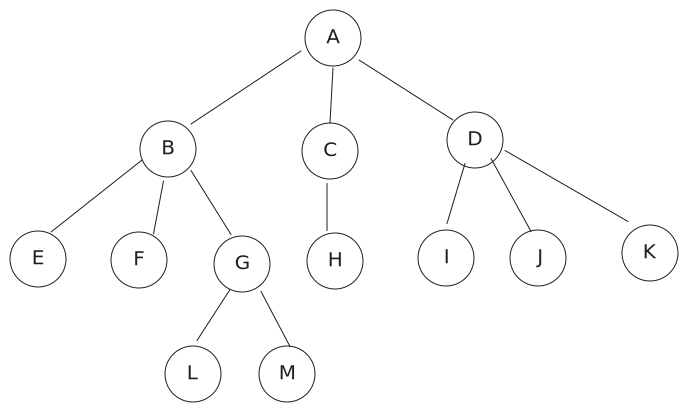
\includegraphics[width=0.8\textwidth]{./figure/pdf/cropped/tree.pdf}
  \caption{树的逻辑表示}
  \label{fig:tree}
\end{figure}
\subsection{树的基本术语}
下面介绍树的常用术语:

\begin{enumerate}
  \item \textbf{结点的度与树的度}:树中某个结点的子树的个数称为该结点的度(degree of node)。
  树中所有结点的度中的最大值称为树的度(degree of tree),通常将度为 $m$ 的树称为 $m$ 次树($m$-ary tree)。
  例如,图\ref{fig:tree} 是一棵 3 次树。

  \item \textbf{分支结点与叶子结点}:树中度不为零的结点称为非终端结点,又叫分支结点(branch)。
  度为零的结点称为叶子结点(leaf)。在分支结点中,每个结点的分支数就是该结点的度。如对于度为 1 的结点,其分支数为 1,
  被称为单分支结点;对于度为 2 的结点,其分支数为 2,被称为双分支结点,依此类推。例如,在图\ref{fig:tree}所示的树中,$B, C$ 和 $D$ 是分支结点,而 $E, F$ 和 $G$ 是叶子结点。

  \item \textbf{路径与路径长度}:对于树中的任意两个结点 $A$ 和 $B$,若树中存在一个结点序列 $(A_1, A_2, \dots, A_n)$ 
  使得序列中除 $A_1$ 和 $A_n$ 以外的任一结点都是其在序列中的前一个结点的后继结点,
  则称该结点序列为由 $A$ 到 $B$ 的一条路径(path)。路径长度(path length)是该路径所通过的结点数目减 1(即路径上分支数目)。
  显然,从树的根结点到树中其余结点均存在一条路径。例如,在图 \ref{fig:tree} 所示的树中,从 $A$ 到 $K$ 的路径为 $(A, D, I, K)$,其长度为 3,而 $(K, I, D, A)$ 为从 $K$ 到 $A$ 的逆路径。

  \item \textbf{孩子结点、双亲结点和兄弟结点}:在一棵树中,每个结点的后继结点被称为该结点的孩子结点(children)。相
  应地,该结点被称为孩子结点的双亲结点(parent)。具有同一双亲结点的孩子结点互为兄弟结点(sibling)。
  进一步推广这些关系,可以把每个结点对应子树中的所有结点(除自身外)称为该结点的子孙结点(descendant),
  把从根结点到达某个结点的路径上经过的所有结点(除自身外)称为该结点的祖先结点(ancestor)。例如,在图 \ref{fig:tree} 所示的树中,结点 $B, C, D$ 互为兄弟结点,结点 $D$ 的子孙结点有 $F, I, K, L$ 和 $M$,结点 $F$ 的祖先结点有 $A$ 和 $D$。

  \item \textbf{结点深度与树的高度}:结点深度(depth)是从树根开始定义的,根结点为第一层,它的孩子结点为第二层,
  依此类推,一个结点所在的层次为其双亲结点的层次加 1。树中结点的最大层次称为树的高度(height of tree)或树的深度(
  depth of tree)。

  \item \textbf{有序树和无序树}:若树中各结点的子树是按照一定的次序从左向右安排的,且相对次序是不能随意变换的,
  则称为有序树(ordered tree),否则称为无序树(unordered tree)。一般情况下,如果没有特别说明,默认树都是指有序树。

  \item \textbf{森林}:$m \ (m \geq 0)$ 个互不相交的树的集合称为森林(forest)。
  把含有多棵子树的树的根结点删去就成了森林(forest)。反之,给 $m \ (m \geq 1)$ 棵独立的树加上一个根结点,
  并把这 $m$ 棵树作为该结点的子树,则森林就变成了一棵树。
\end{enumerate}
\subsection{树的基本性质}
\subsection{树的基本性质}

\begin{enumerate}
  \item \textbf{树中的结点数等于所有结点的度数加 1}:
  \begin{itemize}
    \item \textbf{证明}:不难想象,除根结点以外,每个结点有且仅有一个指向它的前驱结点。也就是说每个结点和指向它的分支一一对应。
    假设树中一共有 $b$ 个分支,那么除了根结点,整个树就包含有 $b$ 个结点,所以整个树的结点数就是这 $b$ 个结点加上根结点,设为 $n$,则 $n = b + 1$。而分支数 $b$ 也就是所有结点的度数,证毕。
  \end{itemize}

  \item \textbf{度为 $m$ 的树中第 $i$ 层上至多有 $m^{i-1}$ 个结点($i \geq 1$)}:
  \begin{itemize}
    \item \textbf{证明}(数学归纳法):
    \begin{itemize}
      \item 首先考虑 $i = 1$ 的情况:第一层只有根结点,即一个结点,$i = 1$ 带入式子满足。
      \item 假设第 $i-1$ 层满足这个性质,第 $i-1$ 层最多有 $m^{i-2}$ 个结点。
      \item 又因为树的度为 $m$,所以对于第 $i-1$ 层的每个结点,最多有 $m$ 个孩子结点。所以第 $i$ 层的结点数最多是第 $i-1$ 层的 $m$ 倍,所以第 $i$ 层上最多有 $m^{i-1}$ 个结点。
    \end{itemize}
  \end{itemize}

  \item \textbf{高度为 $h$ 的 $m$ 叉树至多有 $\frac{m^h - 1}{m - 1}$ 个结点}。

  \item \textbf{具有 $n$ 个结点的 $m$ 叉树的最小高度为 $\log_m(n(m-1)+1)$}。
\end{enumerate}


\section{二叉树}
二叉树是一个有限的结点集合,这个集合或者为空,或者由一个根结点和两棵互不相交的、分别称为根结点的左子树和右子树的二叉树组成。

\subsection{二叉树的定义}

\subsection{二叉树的定义}

\begin{itemize}
  \item 二叉树是 $n$ ($n \geq 0$) 个结点的有限集合:
  \begin{enumerate}
    \item 空二叉树,即 $n = 0$。
    \item 由一个根结点和两个互不相交的被称为根的左子树和右子树组成。左子树和右子树又分别是一棵二叉树。
  \end{enumerate}
  \item 二叉树的特点:
  \begin{enumerate}
    \item 每个结点最多有两棵子树。
    \item 左右子树有顺序,不能随意颠倒。
  \end{enumerate}
\end{itemize}

\textbf{二叉树与度为 2 的树的区别}

\begin{itemize}
  \item 度为 2 的树中至少有一个结点的度为 2,而二叉树没有这个要求。
  \item 度为 2 的树不区分左右子树,而二叉树严格区分左右子树。
\end{itemize}


二叉树的五种基本形态如图\ref{fig:binary_tree}所示:

\begin{itemize}
  \item \textbf{空二叉树}:没有任何结点的二叉树。
  \item \textbf{只有一个根结点}:只有一个根结点,没有左子树和右子树。
  \item \textbf{只有左子树}:只有左子树,没有右子树。
  \item \textbf{只有右子树}:只有右子树,没有左子树。
  \item \textbf{左右子树都有}:既有左子树,又有右子树。
\end{itemize}



\begin{figure}[h]
  \centering
  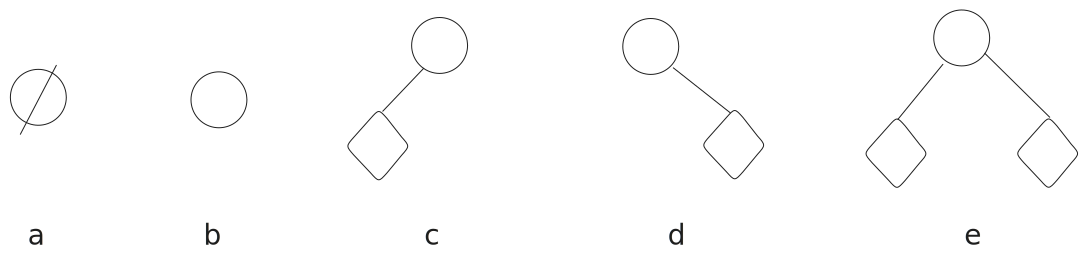
\includegraphics[width=0.8\textwidth]{./figure/pdf/cropped/fiveBTree.pdf}
  \caption{二叉树的五种基本形态}
  \label{fig:binary_tree}
\end{figure}




\subsection{特殊二叉树}

\subsubsection{满二叉树}

在一颗二叉树中,如果所有分支结点都存在左子树和右子树,并且所有叶子结点都在同一层上,这样的二叉树称为满二叉树。如图\ref{fig:full_binary_tree}所示。

\begin{figure}[h]
  \centering
  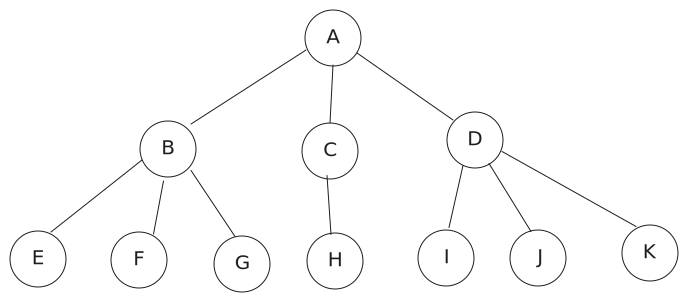
\includegraphics[width=0.8\textwidth]{./figure/pdf/cropped/fullBTree.pdf}
  \caption{满二叉树}
  \label{fig:full_binary_tree}
\end{figure}

非空满二叉树的特点如下:

\begin{itemize}
  \item 叶子结点只能出现在最下一层。
  \item 非叶子结点的度一定是 2。
  \item 在同样深度的二叉树中,满二叉树的结点个数最多,叶子数最多。
  \item 高度为 $h$ 的满二叉树,共有 $2^h - 1$ 个结点。
  \end{itemize}

\subsubsection{完全二叉树}

在一颗二叉树中,最多只有最下面的两层结点的度数可以小于 2,并且最下一层的结点都集中在该层最左边的若干位置上,这样的二叉树称为完全二叉树。如图\ref{fig:complete_binary_tree}所示。
如图\ref{fig:complete_binary_tree}所示。

\begin{figure}[h]
  \centering
  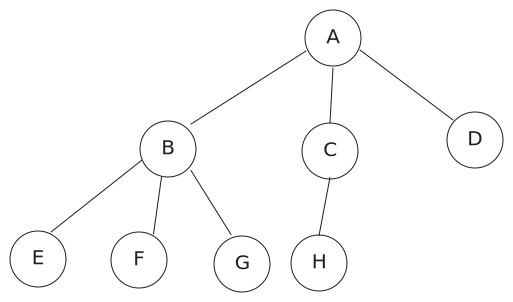
\includegraphics[width=0.6\textwidth]{./figure/pdf/cropped/comBTree.pdf}
  \caption{完全二叉树}
  \label{fig:complete_binary_tree}

\end{figure}


非空完全二叉树的特点如下:

\begin{itemize}
  \item 叶子结点只能出现在最下两层。
  \item 最下层的叶子结点都集中在该层最左边的若干位置上。
  \item 如果有度为 1 的结点,只可能有一个,且一定是最下层的最右边的结点。
  \item 按层序编号时,一旦出现编号为$i$的结点是叶子结点或只有左孩子,则编号为$i$的结点之后的结点必须都是叶子结点。
  \item 非叶子结点的度一定是 2。
  \item 在同样深度的二叉树中,完全二叉树的结点个数最多,叶子数最多。
  \item 高度为 $h$ 的完全二叉树,共有 $2^{h-1}$ 至 $2^h - 1$ 个结点。
  \item 当结点总数$n$为奇数时,$n_1 = 0$ ,为偶数时,$n_1 = 1$。
  \end{itemize}

\subsection{二叉树的性质}

二叉树相关性质如下:

\begin{enumerate}
  \item \textbf{非空二叉树上的叶子结点数等于度为 2 的结点数加 1}。
  \item \textbf{第 $i$ 层上的结点数最多为 $2^{i-1}$}。
  \item \textbf{深度为 $k$ 的二叉树至多有 $2^k - 1$ 个结点}。
  \item \textbf{对任何一棵非空二叉树 $T$,若 $n_0$ 表示叶子结点的个数,$n_1$ 表示度为 1 的结点个数,$n_2$ 表示度为 2 的结点个数,则 $n_0 = n_2 + 1$}。
  \item \textbf{具有 $n$ 个结点的完全二叉树的深度为 $\lfloor \log_2 n \rfloor + 1$}。
  \item \textbf{具有 $n$ 个结点的完全二叉树,从上到下、从左到右编号,对任意结点 $i$ 有}:
  \begin{itemize}
    \item \textbf{若 $i = 1$,则结点 $i$ 是二叉树的根结点,无双亲;}
    \item \textbf{若 $i > 1$,则其双亲是 $\lfloor i/2 \rfloor$;}
    \item \textbf{若 $2i \leq n$,则结点 $i$ 的左孩子是 $2i$;}
    \item \textbf{若 $2i + 1 \leq n$,则结点 $i$ 的右孩子是 $2i + 1$。}
  \end{itemize}
\end{enumerate}
\section{二叉树的存储结构}

\subsection{顺序存储结构}
二叉树的顺序存储结构就是用一组地址连续的存储单元来存放二叉树的数据元素,因此必须确定好树中各数据元素的存放次序,使得各数据元素在这个存放次序中的相互位置能反映出数据元素之间的逻辑关系。

对于完全二叉树和满二叉树,树中结点的层序编号可以唯一地反映出结点之间的逻辑关系,所以可以用一维数组按从上到下、从左到右的顺序存储树中的所有结点值,通过数组元素的下标关系反映完全二叉树或满二叉树中结点之间的逻辑关系。

例如,上图所示的完全二叉树对应的顺序存储结构如下图所示,编号为 $i$ 的结点值存放在数组下标为$i$的元素中(`\#` 表示空结点)。
由于 C/C++ 语言中的数组下标从 0 开始,这里为了一致性而没有使用下标为 0 的数组元素。

\begin{figure}[h]
  \centering
  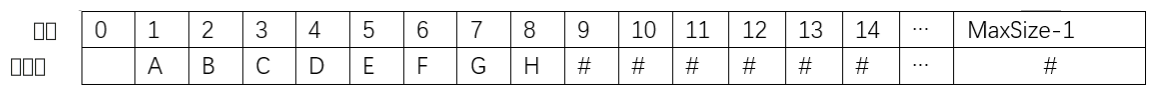
\includegraphics[width=0.8\textwidth]{./figure/pdf/cropped/seqBTree.pdf}
  \caption{完全二叉树的顺序存储结构}
  \label{fig:seq_binary_tree}
\end{figure}

显然,对于满二叉树和完全二叉树而言,这样的做法是十分方便的。但是如果是一般的二叉树,我们若还想让下标满足完全二叉树的特性,
就不得不增添许多的空结点,这就使得空间浪费严重。所以一般而言,对于一般二叉树采用下面介绍的链式存储方式。
\subsection{链式存储结构}

二叉树的链式存储结构是指用链表的方式存储二叉树。二叉树的链式存储结构是一种递归的定义方式,即二叉树是由结点构成的,
而结点又是由左右子树构成的。

二叉树链式存储结构的标准存储结构如图\ref{fig:binary_tree_node}所示,其中 $data$ 为结点的数据域,$lchild$ 和 $rchild$ 分别为结点的左孩子和右孩子指针域。

\begin{figure}[h]
  \centering
  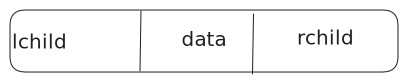
\includegraphics[width=0.5\textwidth]{./figure/pdf/cropped/BTreeStruct.pdf}
  \caption{二叉树的链式存储结构}
  \label{fig:binary_tree_node}
\end{figure}

二叉链中结点的定义如下:

\begin{lstlisting}[language=C++, caption={二叉树链式存储结构}]
  typedef struct BiTNode {
    TElemType data;
    struct BiTNode *lchild, *rchild;
  } BiTNode, *BiTree;
\end{lstlisting}

其中,$TElemType$ 为二叉树结点的数据类型,$BiTNode$ 为二叉树结点的结构体,$BiTree$ 为指向二叉树结点的指针。

由于本章后面的算法均用到二叉链存储结构,为此将其类型定义存储在头文件 $BiTree.h$ 中,方便后续的引用。

例如,图 \ref{fig:binary_tree_link}(左) 所示的二叉树的链式存储结构如图\ref{fig:binary_tree_link}(右)所示。

\begin{figure}[h]
  \centering
  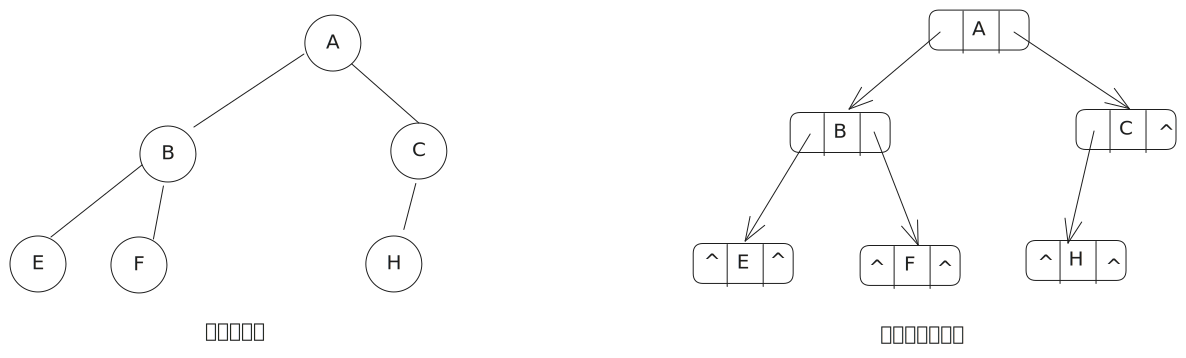
\includegraphics[width=0.8\textwidth]{./figure/pdf/cropped/BTreeGraph.pdf}
  \caption{二叉树的链式存储结构}
  \label{fig:binary_tree_link}
\end{figure}

\section{二叉树的遍历}


\subsection{遍历的定义}
\section{二叉树的遍历}

二叉树的遍历是指按照一定的次序访问二叉树中的所有结点,并且每个结点仅被访问一次的过程。它是二叉树最基本的运算,是二叉树中所有其他运算实现的基础。

一棵二叉树由 3 个部分(即根结点、左子树和右子树)构成,可以从任何部分开始遍历,所以有 $3!$(即 6)种遍历方法。若规定子树的遍历总是先左后右(先右后左与之对称),
则对于非空二叉树,可得到以下 3 种递归的遍历方法,即先序遍历、中序遍历和后序遍历。另外,还有一种常见的层次遍历方法。

\subsection{递归遍历}

二叉树的递归遍历是指在遍历过程中,每个结点的左子树和右子树都是通过递归调用同一个遍历函数来实现的。具体又可分为先序遍历、中序遍历和后序遍历。我们将以图
\ref{fig:binary_tree_link}所示的二叉树为例,介绍这三种递归遍历方法。

\begin{figure}
  \centering
  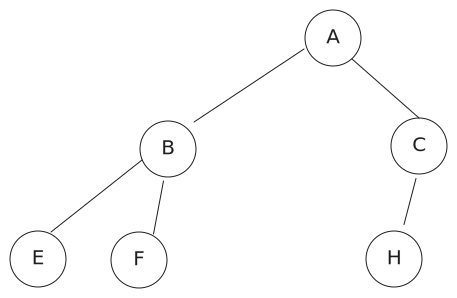
\includegraphics[width=0.8\textwidth]{./figure/pdf/cropped/oneBTree.pdf}
  \caption{二叉树的链式存储结构}
  \label{fig:binary_tree_link}
\end{figure}

\subsubsection{先序遍历}

先序遍历是指先访问根结点,然后依次先序遍历左子树和右子树。对于图\ref{fig:binary_tree_link}所示的二叉树,先序遍历的结果为 $ABEFCH$。

先序遍历的代码如\ref{code:precode}所示:

\begin{lstlisting}[language=C++, caption={先序遍历}, label={code:precode}]
  void PreOrderTraverse(BiTree T) {
    if (T == NULL) {
      return;
    }
    printf("%c", T->data);
    PreOrderTraverse(T->lchild);
    PreOrderTraverse(T->rchild);
  }
\end{lstlisting}

观察代码我们可以发现,先序遍历的过程就是先访问根结点,然后递归地先序遍历左子树和右子树。而对于递归而言,有两个关键点:

\begin{itemize}
  \item 递归的结束条件:对于二叉树的遍历,递归的结束条件就是当前结点为空。
  \item 递归的递推关系:对于先序遍历,递推关系就是先访问当前结点,然后递归地先序遍历左子树和右子树。
  \end{itemize}





\subsubsection{中序遍历}

中序遍历是指先中序遍历左子树,然后访问根结点,最后中序遍历右子树。对于图\ref{fig:binary_tree_link}所示的二叉树,中序遍历的结果为 $EBFAHC$。

中序遍历的代码如\ref{code:incode}所示:

\begin{lstlisting}[language=C++, caption={中序遍历}, label={code:incode}]
  void InOrderTraverse(BiTree T) {
    if (T == NULL) {
      return;
    }
    InOrderTraverse(T->lchild);
    printf("%c", T->data);
    InOrderTraverse(T->rchild);
  }

\end{lstlisting}

观察代码我们可以发现,中序遍历的过程就是先递归地中序遍历左子树,然后访问当前结点,最后递归地中序遍历右子树。
\subsubsection{后序遍历}


后序遍历是指先后序遍历左子树和右子树,然后访问根结点。对于图\ref{fig:binary_tree_link}所示的二叉树,后序遍历的结果为 $EFBHCA$。

后序遍历的代码如\ref{code:postcode}所示:

\begin{lstlisting}[language=C++, caption={后序遍历} , label={code:postcode}]
  void PostOrderTraverse(BiTree T) {
    if (T == NULL) {
      return;
    }
    PostOrderTraverse(T->lchild);
    PostOrderTraverse(T->rchild);
    printf("%c", T->data);
  }

\end{lstlisting}

观察代码我们可以发现,后序遍历的过程就是先递归地后序遍历左子树和右子树,然后访问当前结点。
\subsection{非递归遍历}

递归遍历的缺点是递归调用时需要保存函数调用信息,因此会占用较多的栈空间。为了解决这个问题,可以使用非递归遍历的方法。


\subsubsection{先序遍历}

由先序遍历过程可知,先访问根结点,再遍历左子树,最后遍历右子树。所以先访问根结点及其所有左下结点,但是因为在二叉链表中并没有指向双亲结点的指针,
所以我们需要将已访问过的结点存入栈中。此时栈顶结点要么没有左子树,要么左子树已遍历过,所以转向它的右子树,对右子树的处理与上述过程类似。

先序遍历的非递归算法如\ref{code:precode2}所示:

\begin{lstlisting}[language=C++, caption={先序遍历}, label={code:precode2}]
  void PreOrderTraverse(BiTree T) {
    InitStack(S);
    BiTree p = T;
    while (p != NULL || !StackEmpty(S)) {//栈不空或者p不空
      if (p != NULL) {//一直向左并将沿途结点压入栈
        printf("%c", p->data);//访问结点
        Push(S, p);
        p = p->lchild;
      } else {//结点弹出栈
        Pop(S, p);
        p = p->rchild;
      }
    }
  }
\end{lstlisting}

注:外循环中的条件是指针p不为空或者栈不为空,这是因为,p是指向当前所要访问元素,只要它不为空我们就要就行访问和入栈,当p一路向左直至为空的时候,
说明此时应该转头去访问双亲结点(如果有)的右子树了,
也就是这里我们要去判断栈是否为空,若不为空,我们便同样要进入循环,进行类似的操作。同学们对于这类较复杂的算法过程一定要手动进行模拟,不能光靠想。

先序遍历过程中指针和栈的变化如表\ref{tab:preorder_stack}所示。

\begin{table}[h!]
  \centering
  \caption{先序遍历过程中指针和栈的变化}
  \begin{tabular}{|c|c|c|c|}
  \hline
  \textbf{p指针的值} & \textbf{当前访问结点} & \textbf{当前栈的操作} & \textbf{当前栈内元素(栈底 $\to$ 栈顶)} \\ \hline
  A & A & A入栈 & A \\ \hline
  B & B & B入栈 & A B \\ \hline
  E & E & E入栈 & A B E \\ \hline
  NULL &  &  & A B E \\ \hline
  E &  & E出栈 & A B \\ \hline
  NULL &  &  & A B \\ \hline
  B &  & B出栈 & A \\ \hline
  F & F & F入栈 & A F \\ \hline
  NULL &  &  & A F \\ \hline
  F &  & F出栈 & A \\ \hline
  NULL &  &  & A \\ \hline
  A &  & A出栈 &  \\ \hline
  C & C & C入栈 & C \\ \hline
  H & H & H入栈 & C H \\ \hline
  ... & ... & ... & ... \\ \hline
  \end{tabular}
  \label{tab:preorder_stack}
  \end{table}
\subsubsection{中序遍历}
中序非递归算法是在前面先序遍历非递归算法的基础上修改的,中序遍历顺序是左子树 根结点 右子树 所以需要将根结点及其左下结点依次进栈,但还不能访问,
因为它的左子树没有遍历.当达到根结点的最左下结点时,它是中序序列的开始结点,也是栈顶节点,出栈并访问它,然后转向它的右子树,对右子树的处理与上述过程类似.

中序遍历的非递归算法如\ref{code:incode2}所示:

\begin{lstlisting}[language=C++, caption={中序遍历}, label={code:incode2}]
  void InOrderTraverse(BiTree T) {
    InitStack(S);
    BiTree p = T;
    while (p != NULL || !StackEmpty(S)) {
      if (p != NULL) {
        Push(S, p);
        p = p->lchild;
      } else {
        Pop(S, p);
        printf("%c", p->data);
        p = p->rchild;
      }
    }
  }
\end{lstlisting}

中序遍历过程中指针和栈的变化如表\ref{tab:inorder_stack}所示。

\begin{table}[h!]
  \centering
  \caption{中序遍历过程中指针和栈的变化}
  \begin{tabular}{|c|c|c|c|}
  \hline
  \textbf{p指针的值} & \textbf{当前访问结点} & \textbf{当前栈操作} & \textbf{当前栈内元素(栈底 $\to$ 栈顶)} \\ \hline
  A &  & A入栈 & A \\ \hline
  B &  & B入栈 & A B \\ \hline
  E &  & E入栈 & A B E \\ \hline
  NULL &  &  & A B E \\ \hline
  E & E & E出栈 & A B \\ \hline
  NULL &  &  & A B \\ \hline
  B & B & B出栈 & A \\ \hline
  F &  & F入栈 & A F \\ \hline
  NULL &  &  & A F \\ \hline
  F & F & F出栈 & A \\ \hline
  NULL &  &  & A \\ \hline
  A & A & A出栈 &  \\ \hline
  C &  & C入栈 & C \\ \hline
  H &  & H入栈 & C H \\ \hline
  NULL &  &  & C H \\ \hline
  H & H & H出栈 & C \\ \hline
  NULL &  &  & C \\ \hline
  C & C & C出栈 &  \\ \hline
  NULL &  &  & 程序结束 \\ \hline
  \end{tabular}
  \label{tab:inorder_stack}
  \end{table}



\subsubsection{后序遍历}
\subsubsection{后序遍历}

后序遍历的顺序是:先访问左子树,再访问右子树,最后访问根结点。为了实现这一顺序,我们需要先将根结点及其左下结点依次压入栈中。即使栈顶结点 $p$ 的左子树已经遍历完或为空,也不能立即访问结点 $p$,因为它的右子树还没有遍历。只有当结点 $p$ 的右子树也遍历完后,才能访问结点 $p$。因此,后序遍历的实现比前序和中序遍历更复杂,因为它有更多的条件限制。

\textbf{模拟遍历流程}

1. 首先将 $A, B, E$ 入栈,发现 $E$ 没有左孩子也没有右孩子,直接输出 $E$,然后将 $E$ 出栈。

2. 此时栈顶元素为 $B$,访问 $B$,发现 $B$ 有右孩子,将右孩子 $F$ 入栈。

3. $F$ 和 $E$ 类似,输出 $F$ 后将其出栈。

4. 栈顶元素仍为 $B$,但此时 $B$ 的右孩子已经被访问过了,所以直接输出 $B$。

5. 栈顶元素变为 $A$,$A$ 有右孩子且未被访问,将右孩子 $C$ 入栈。

6. 按照同样的逻辑,继续遍历,直到栈为空。

\textbf{需要解决的问题}

在后序遍历中,我们需要判断栈顶元素的右孩子是否已经被访问过。为了解决这个问题,可以在每次访问结点时,将当前结点标记存储起来。当退回到栈顶元素时,检查当前结点是否是栈顶元素的右孩子:

如果是,说明右子树已经被访问过,可以直接访问栈顶元素。

如果不是,说明右子树还未遍历,需要继续处理右子树。

通过这种方法,我们可以正确地实现后序遍历。

后序遍历的非递归算法如\ref{code:postcode2}所示:

\begin{lstlisting}[language=C++, caption={后序遍历}, label={code:postcode2}]
  void PostOrderTraverse(BiTree T) {
    InitStack(S);
    BiTree p = T;
    BiTree r = NULL;
    while (p != NULL || !StackEmpty(S)) {
      if (p != NULL) {
        Push(S, p);
        p = p->lchild;
      } else {
        GetTop(S, p);
        if (p->rchild != NULL && p->rchild != r) {
          p = p->rchild;
        } else {
          Pop(S, p);
          printf("%c", p->data);
          r = p;
          p = NULL;
        }
      }
    }
  }
\end{lstlisting}

后序遍历过程中指针和栈的变化如表\ref{tab:postorder_stack}所示。
\begin{table}[h!]
  \centering
  \caption{后序遍历过程中指针和栈的变化}
  \begin{tabular}{|c|c|c|c|c|}
  \hline
  \textbf{p指针的值} & \textbf{r指针的值} & \textbf{当前访问元素} & \textbf{当前栈操作} & \textbf{当前栈内元素(栈底 $\to$ 栈顶)} \\ \hline
  A & NULL &  & A入栈 & A \\ \hline
  B & NULL &  & B入栈 & AB \\ \hline
  E & NULL &  & E入栈 & ABE \\ \hline
  NULL & NULL &  &  & ABE \\ \hline
  E(没有右孩子) & NULL & E & E出栈 & AB \\ \hline
  NULL & E &  &  & AB \\ \hline
  B & E &  &  & AB \\ \hline
  F & E &  & F入栈 & ABF \\ \hline
  NULL & E &  &  & ABF \\ \hline
  F(没有右孩子) & F & F & F出栈 & AB \\ \hline
  B(右孩子与r同) & F & B & B出栈 & A \\ \hline
  A(右孩子不等于r,继续向右遍历) & B &  &  & A \\ \hline
  C & B &  & C入栈 & AC \\ \hline
  H & B &  & H入栈 & ACH \\ \hline
  NULL & B &  &  & ACH \\ \hline
  H(没有右孩子) & B & H & H出栈 & AC \\ \hline
  C(没有右孩子) & H & C & C出栈 & A \\ \hline
  A(右孩子与r同) & C & A & A出栈 & 程序结束 \\ \hline
  \end{tabular}
  \label{tab:postorder_stack}
  \end{table}
\subsection{层次遍历}

层次遍历是指按照从上到下、从左到右的顺序,依次访问二叉树中的每个结点。层次遍历需要借助队列来实现,其基本思想是:

\begin{itemize}
  \item 先将根结点入队。
  \item 当队列不为空时,执行以下操作:
  \begin{itemize}
    \item 将队头结点出队并访问。
    \item 将队头结点的左孩子入队。
  \end{itemize}
\end{itemize}

层次遍历的代码如\ref{code:levelcode}所示:

\begin{lstlisting}[language=C++, caption={层次遍历}, label={code:levelcode}]
  void LevelOrderTraverse(BiTree T) {
    InitQueue(Q);
    BiTree p;
    EnQueue(Q, T);
    while (!QueueEmpty(Q)) {
      DeQueue(Q, p);
      printf("%c", p->data);
      if (p->lchild != NULL) {
        EnQueue(Q, p->lchild);
      }
      if (p->rchild != NULL) {
        EnQueue(Q, p->rchild);
      }
    }
  }
\end{lstlisting}



\section{二叉树的基本运算及其实现}
二叉树的基本运算包括创建二叉树、清空二叉树、销毁二叉树、判断二叉树是否为空、求二叉树的深度、求二叉树的结点个数等。这些运算是二叉树的基本操作,也是其他运算的基础。
\subsection{二叉树的创建}

大家想想我们在手画一棵二叉树的步骤,是不是先画出根结点,然后画出分支,再画出其孩子结点。如此循环往复。其实,所有的算法代码都是我们实际问题的模拟。我们先画的是根结点,那么我们就采取先序遍历来创建一棵二叉树。

我们之前学习过先序遍历的递归代码,现在让我们看看如何将最基本的递归遍历代码改造为创建一棵二叉树的代码。

首先,先序遍历的代码如下:

\begin{lstlisting}[language=C++, caption={先序遍历}]
  void PreOrderTraverse(BiTree T) {
    if (T == NULL) {
      return;
    }
    printf("%c", T->data);
    PreOrderTraverse(T->lchild);
    PreOrderTraverse(T->rchild);
  }
\end{lstlisting}

首先,我们应该明确,创建一棵二叉树的过程就是根据先序遍历的顺序,依次输入结点的值,当输入的值为某个特定值(例如 \texttt{\#})时,表示该结点为空。代码如 \ref{code:create} 所示。

\begin{lstlisting}[language=C++, caption={创建二叉树}, label={code:create}]
  void CreateBiTree(BiTree &T) {
    TElemType ch;
    scanf("%c", &ch);
    if (ch == '#') {
      T = NULL;
    } else {
      T = (BiTree)malloc(sizeof(BiTNode));
      if (!T) {
        exit(OVERFLOW);
      }
      T->data = ch;
      CreateBiTree(T->lchild);
      CreateBiTree(T->rchild);
    }
  }
\end{lstlisting}

代码中,我们首先输入一个字符,如果该字符为 \texttt{\#},则表示该结点为空,否则我们为该结点分配内存空间,并将该字符赋值给该结点的数据域。接着,我们递归地创建左子树和右子树。

\subsection{二叉树的销毁}

二叉树的销毁是指将二叉树中的所有结点释放掉,使其成为一个空树。销毁二叉树的代码如\ref{code:destroy}所示。

\begin{lstlisting}[language=C++, caption={销毁二叉树}, label={code:destroy}]
  void DestroyBiTree(BiTree &T) {
    if (T == NULL) {
      return;
    }
    DestroyBiTree(T->lchild);
    DestroyBiTree(T->rchild);
    free(T);
    T = NULL;
  }
\end{lstlisting}

销毁二叉树的过程就是递归地销毁左子树和右子树,然后释放根结点的内存空间。

\subsection{二叉树的清空}

二叉树的清空是指将二叉树中的所有结点清空,使其成为一个空树。清空二叉树的代码如\ref{code:clear}所示。

\begin{lstlisting}[language=C++, caption={清空二叉树}, label={code:clear}]
  void ClearBiTree(BiTree &T) {
    if (T == NULL) {
      return;
    }
    ClearBiTree(T->lchild);
    ClearBiTree(T->rchild);
    T = NULL;
  }

\end{lstlisting}

清空二叉树的过程就是递归地清空左子树和右子树,然后将根结点置为空。

\subsection{二叉树的判空}

二叉树的判空是指判断二叉树是否为空。判空的代码如\ref{code:empty}所示。

\begin{lstlisting}[language=C++, caption={判空}, label={code:empty}]
  Status BiTreeEmpty(BiTree T) {
    if (T == NULL) {
      return TRUE;
    } else {
      return FALSE;
    }
  }

\end{lstlisting}

判空的过程就是判断根结点是否为空。

\subsection{二叉树的深度}

二叉树的深度是指二叉树中结点的最大层次。求二叉树的深度的代码如\ref{code:depth}所示。

\begin{lstlisting}[language=C++, caption={求深度}, label={code:depth}]
  int BiTreeDepth(BiTree T) {
    if (T == NULL) {
      return 0;
    }
    int ldepth = BiTreeDepth(T->lchild);
    int rdepth = BiTreeDepth(T->rchild);
    return ldepth > rdepth ? ldepth + 1 : rdepth + 1;
  }

\end{lstlisting}

求深度的过程就是递归地求左子树和右子树的深度,然后取两者中的较大值加 1。

\subsection{二叉树的结点个数}

二叉树的结点个数是指二叉树中结点的个数。求二叉树的结点个数的代码如\ref{code:count}所示。

\begin{lstlisting}[language=C++, caption={求结点个数}, label={code:count}]
  int BiTreeCount(BiTree T) {
    if (T == NULL) {
      return 0;
    }
    return BiTreeCount(T->lchild) + BiTreeCount(T->rchild) + 1;
  }

\end{lstlisting}

求结点个数的过程就是递归地求左子树和右子树的结点个数,然后将两者相加并加 1。

\subsection{求结点值为x的层次}

求结点值为 $x$ 的层次是指求出二叉树中值为 $x$ 的结点所在的层次。求结点值为 $x$ 的层次的代码如\ref{code:level}所示。

\begin{lstlisting}[language=C++, caption={求结点值为x的层次}, label={code:level}]
  int BiTreeLevel(BiTree T, TElemType x) {
    if (T == NULL) {
      return 0;
    }
    if (T->data == x) {
      return 1;
    }
    int llevel = BiTreeLevel(T->lchild, x);
    int rlevel = BiTreeLevel(T->rchild, x);
    if (llevel > 0) {
      return llevel + 1;
    } else if (rlevel > 0) {
      return rlevel + 1;
    } else {
      return 0;
    }
  }

\end{lstlisting}

求结点值为 $x$ 的层次的过程就是递归地求左子树和右子树中值为 $x$ 的结点所在的层次,然后取两者中的较大值加 1。


\section{二叉树的构造}

我们在这个小节中,将介绍二叉树的构造方法,包括根据先序遍历和中序遍历构造二叉树、根据中序遍历和后序遍历构造二叉树、根据层次遍历构造二叉树等。

我们假设二叉树的每个结点的值为单个字符,且不重复。同一颗二叉树具有唯一的先序遍历、中序遍历和后序遍历序列,但不同的二叉树可能具有相同的先序遍历、中序遍历和后序遍历序列。

如图\ref{fig:samePre}所示,5颗不同的二叉树具有相同的先序遍历序列 $ABC$

\begin{figure}[h]
  \centering
  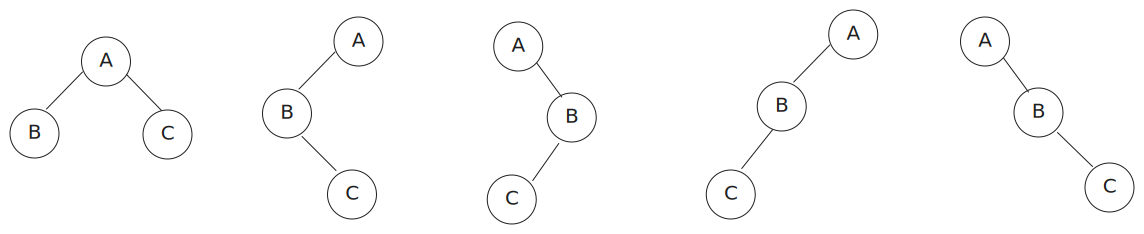
\includegraphics[width=0.8\textwidth]{./figure/pdf/cropped/preBTree.pdf}
  \caption{具有相同先序遍历序列的不同二叉树}
  \label{fig:samePre}
\end{figure}

如图\ref{fig:sameIn}所示,5颗不同的二叉树具有相同的中序遍历序列 $ACB$

\begin{figure}[h]
  \centering
  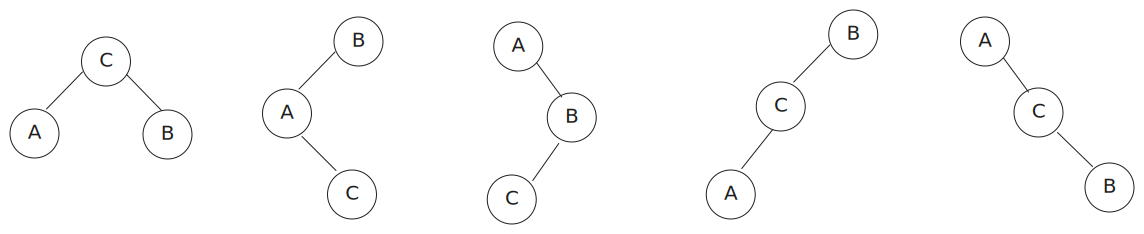
\includegraphics[width=0.8\textwidth]{./figure/pdf/cropped/inBTree.pdf}
  \caption{具有相同中序遍历序列的不同二叉树}
  \label{fig:sameIn}
\end{figure}

如图\ref{fig:samePost}所示,5颗不同的二叉树具有相同的后序遍历序列 $CBA$

\begin{figure}[h]
  \centering
  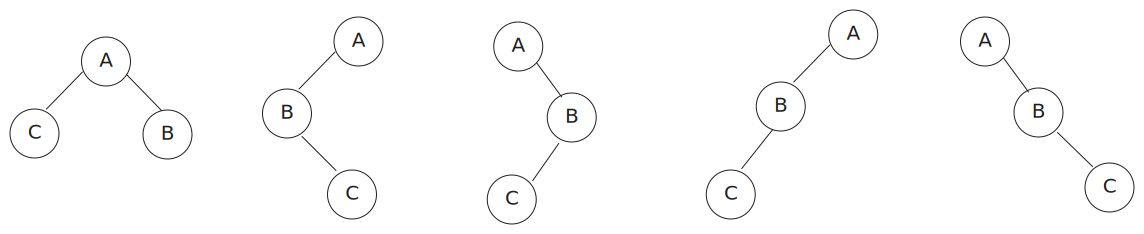
\includegraphics[width=0.8\textwidth]{./figure/pdf/cropped/postBTree.pdf}
  \caption{具有相同后序遍历序列的不同二叉树}
  \label{fig:samePost}
\end{figure}

\subsection{根据先序遍历和中序遍历构造二叉树}

根据先序遍历和中序遍历构造二叉树的基本思想是:

\begin{itemize}
  \item 先序遍历序列的第一个结点为根结点。
  \item 在中序遍历序列中找到根结点,根结点左边的结点为左子树的中序遍历序列,根结点右边的结点为右子树的中序遍历序列。
  \item 根据左子树的中序遍历序列和先序遍历序列,递归地构造左子树。
  \item 根据右子树的中序遍历序列和先序遍历序列,递归地构造右子树。
  \end{itemize}

根据先序遍历和中序遍历构造二叉树的过程如图\ref{fig:preIn}所示。

\begin{figure}[h]
  \centering
  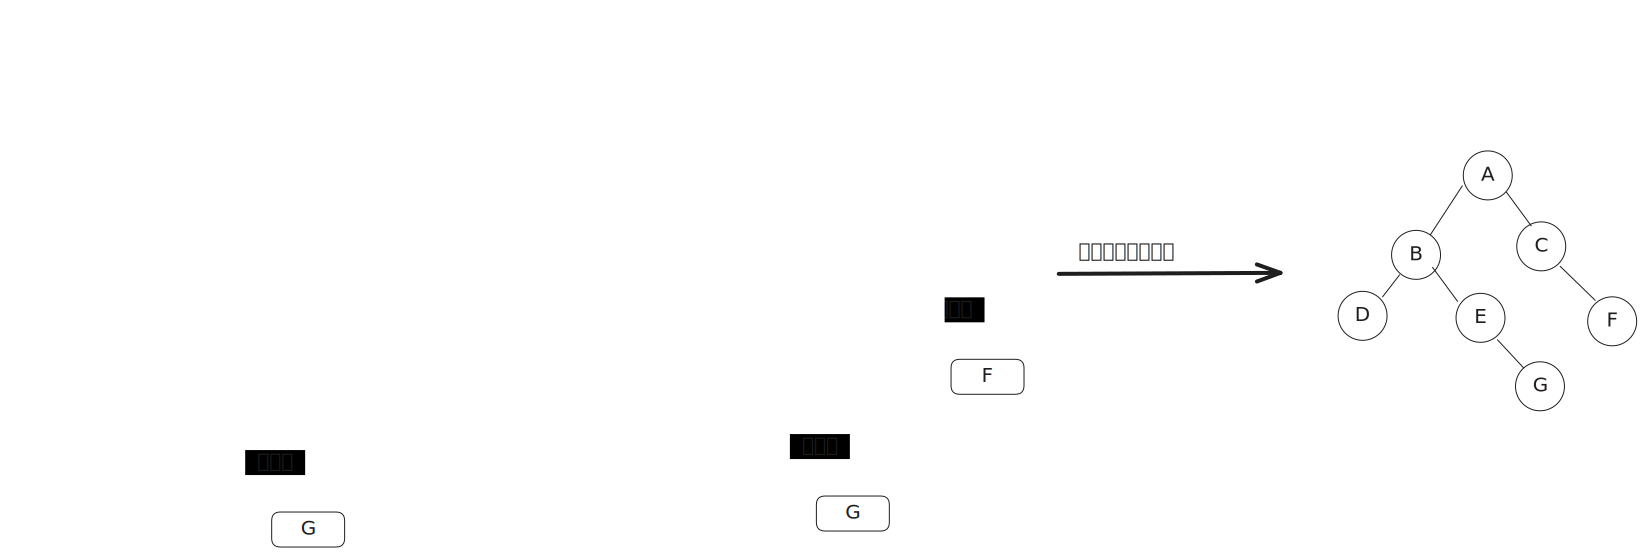
\includegraphics[width=0.8\textwidth]{./figure/pdf/cropped/pre+in.pdf}
  \caption{根据先序遍历和中序遍历构造二叉树}
  \label{fig:preIn}
\end{figure}

根据先序遍历和中序遍历构造二叉树的代码如\ref{code:preIn}所示。

\begin{lstlisting}[language=C++, caption={根据先序遍历和中序遍历构造二叉树}, label={code:preIn}]
  BiTree PreInCreateBiTree(TElemType *pre, TElemType *in, int n) {
    if (n == 0) {
      return NULL;
    }
    BiTree T = (BiTree)malloc(sizeof(BiTNode));
    if (!T) {
      exit(OVERFLOW);
    }
    T->data = *pre;
    int k = 0;
    while (in[k] != *pre) {
      k++;
    }
    T->lchild = PreInCreateBiTree(pre + 1, in, k);
    T->rchild = PreInCreateBiTree(pre + k + 1, in + k + 1, n - k - 1);
    return T;
  }
\end{lstlisting}

代码中,我们首先判断结点个数是否为 0,如果为 0,则返回空树。然后,我们为根结点分配内存空间,并将先序遍历序列的第一个结点赋值给根结点的数据域。接着,我们在中序遍历序列中找到根结点,根结点左边的结点为左子树的中序遍历序列,根结点右边的结点为右子树的中序遍历序列。然后,我们递归地构造左子树和右子树。

\section{线索二叉树}

对于具有 $n$ 个结点的二叉树,当采用二叉链存储结构时,每个结点有两个指针域,总共有 $2n$ 个指针域。又由于只有 $n-1$ 个结点被有效指针域所指向($n$ 个结点中只有根结点没有被有效指针域指向),则共有 $2n - (n-1) = n+1$ 个空链域。

遍历二叉树的结果是一个结点的线性序列,可以利用这些空链域存放指向结点的前驱结点和后继结点的地址。其规定是当某结点的左指针为空时,令该指针指向这个线性序列中该结点的前驱结点;当某结点的右指针为空时,令该指针指向这个线性序列中该结点的后继结点。这样的指向该线性序列中的“前驱结点”和“后继结点”的指针称为线索(thread)。

创建线索的过程称为线索化。线索化的二叉树称为线索二叉树(threaded binary-tree)。

由于遍历方式不同,产生的遍历线性序列也不同,会得到相应的线索二叉树。一般有先序线索二叉树、中序线索二叉树和后序线索二叉树。创建线索二叉树的目的是提高该遍历过程的效率。

那么,在线索二叉树中如何区分左指针指向的是左孩子结点还是前驱结点,右指针指向的是右孩子结点还是后继结点呢?为此,在结点的存储结构上增加两个标志位来区分这两种情况:

\begin{itemize}
  \item 左标志 $ltag$:
  \begin{itemize}
    \item $0$ 表示 $lchild$ 指向左孩子结点;
    \item $1$ 表示 $lchild$ 指向前驱结点。
  \end{itemize}
  \item 右标志 $rtag$:
  \begin{itemize}
    \item $0$ 表示 $rchild$ 指向右孩子结点;
    \item $1$ 表示 $rchild$ 指向后继结点。
  \end{itemize}
\end{itemize}

这样,每个结点的存储结构如下:

\[
\begin{array}{|c|c|c|c|c|}
\hline
\text{ltag} & \text{lchild} & \text{data} & \text{rchild} & \text{rtag} \\
\hline
\end{array}
\]

在某遍历方式的线索二叉树中,若开始结点 $p$ 没有左孩子,将 $p$ 结点的左指针改为线索,其左指针仍为空;若最后结点 $q$ 没有右孩子,将 $q$ 结点的右指针改为线索,其右指针仍为空。对于其他结点 $x$,若它没有左孩子,将左指针改为指向前驱结点的非空线索;若它没有右孩子,将右指针改为指向后继结点的非空线索。

为使创建线索二叉树的算法设计方便,在线索二叉树中再增加一个头结点。头结点的 $data$ 域为空;$lchild$ 指向无线索时的根结点,$ltag$ 为 $0$;$rchild$ 指向按某种方式遍历二叉树时的最后一个结点,$rtag$ 为 $1$。

图\ref{fig:threadedBTree}所示的线索二叉树,其中:
\begin{itemize}
  \item 图\ref{fig:threadedBTree}(a) 是二叉树(中序序列为 $D, B, G, A, E, C, F$);
  \item 图\ref{fig:threadedBTree}(c) 是中序线索二叉树(中序序列为 $D, G, B, A, E, C, F$);
  \item 图\ref{fig:threadedBTree}(b) 是先序线索二叉树(先序序列为 $A, B, D, G, C, E, F$);
  \item 图\ref{fig:threadedBTree}(d) 是后序线索二叉树(后序序列为 $G, D, B, E, F, C, A$)。
\end{itemize}
\begin{figure}[h]
  \centering
  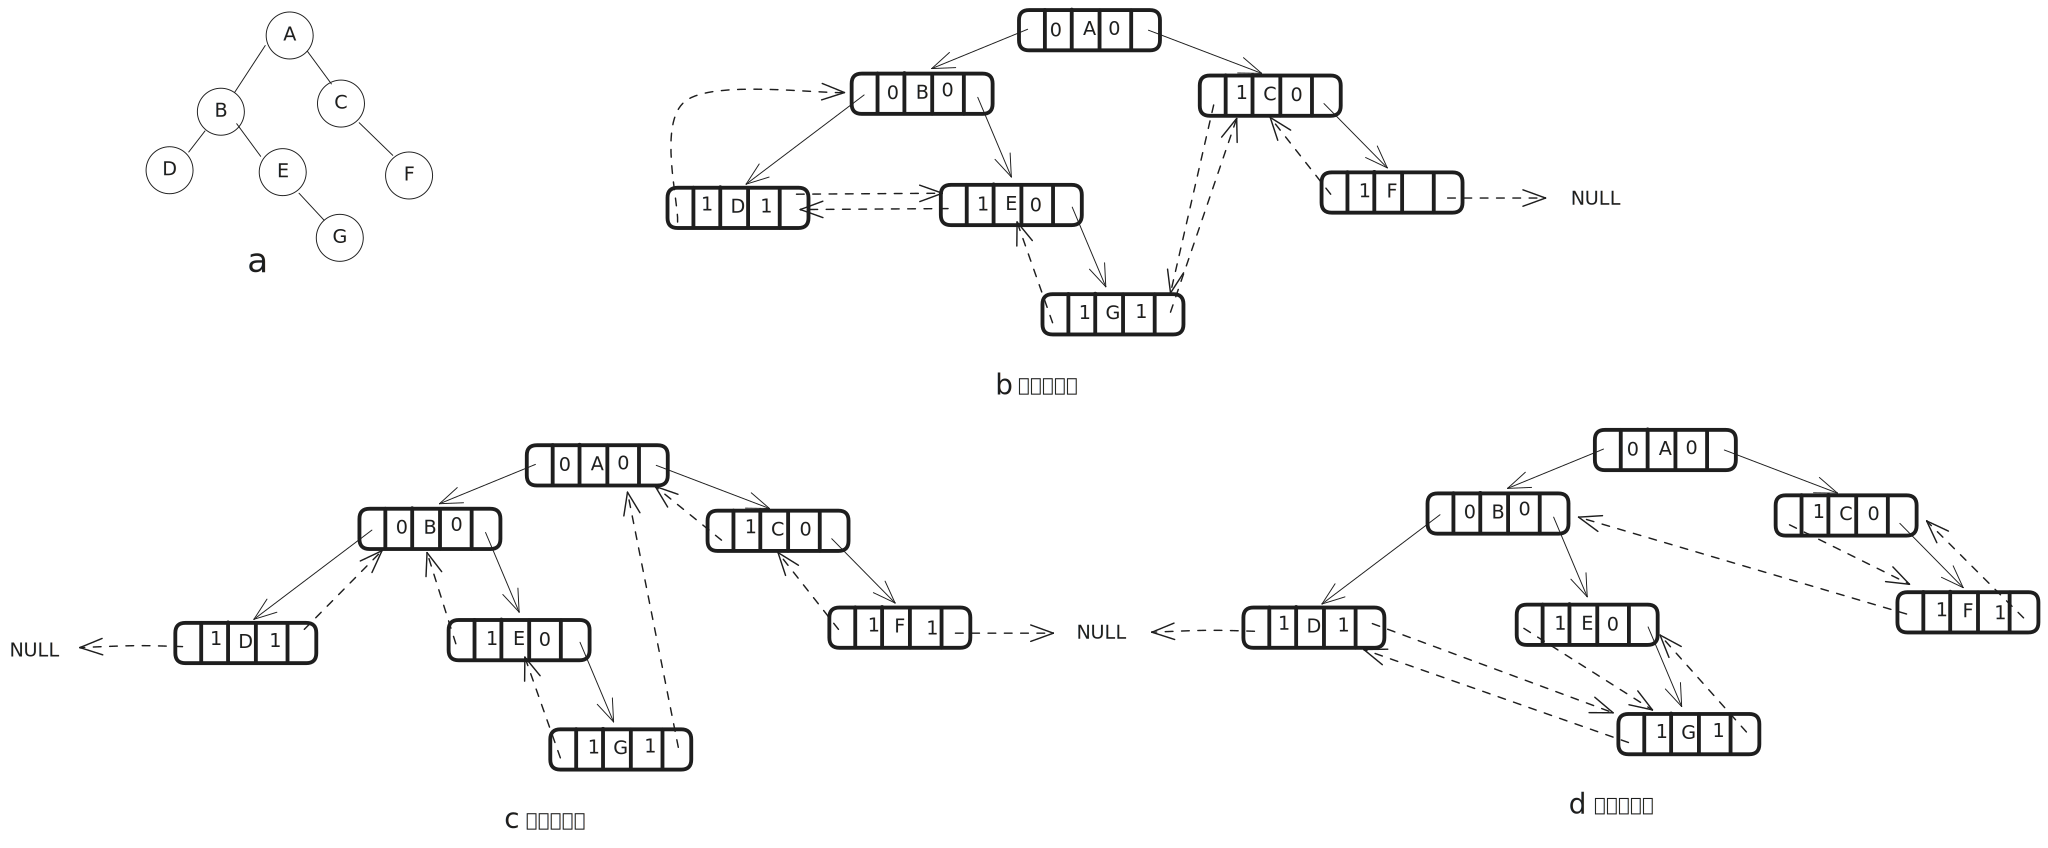
\includegraphics[width=1\textwidth]{./figure/pdf/cropped/threadBTree.pdf}
  \caption{线索二叉树}
  \label{fig:threadedBTree}
\end{figure}
图中的实线表示二叉树原来指针所指的结点,虚线表示线索二叉树所添加的线索。

\subsection{建立线索二叉树}

建立线索二叉树的过程是在遍历二叉树的过程中,将空指针域改为指向前驱结点或后继结点的线索。为了实现线索二叉树,将前面的二叉树的存储结构中的 $ltag$ 和 $rtag$ 
增加到结点中,同时增加一个头结点,头结点的 $lchild$ 指向根结点,$rchild$ 指向最后一个结点。其类型声明如下:

\begin{lstlisting}[language=C++, caption={线索二叉树结点类型定义}]
  typedef struct BiThrNode {
    TElemType data;
    struct BiThrNode *lchild, *rchild;
    int ltag, rtag;
  } BiThrNode, *BiThrTree;
\end{lstlisting}

线索二叉树的建立过程如下:

\begin{itemize}
  \item 若二叉树为空,则线索二叉树为空;
  \item 若二叉树不为空,则按照中序遍历的顺序,将二叉树中的每个结点的 $lchild$ 指针指向其前驱结点,$rchild$ 指针指向其后继结点。
  \end{itemize}

\subsection{中序线索化}

下面以中序线索二叉树为例讨论建立线索二叉树的算法。

\textbf{CreateThread(b)} 算法的功能是将以二叉链存储的二叉树 $T$ 进行中序线索化,并返回线索化后头结点的指针 $root$。\textbf{Thread(p)} 算法的功能是对
以结点 $p$ 为根的二叉树进行中序线索化。在整个算法中,$p$ 总是指向当前被线索化的结点,而 $pre$ 作为全局变量,指向刚访问过的结点。结点 $pre$ 是结点 $p$ 的
前驱结点,结点 $p$ 是结点 $pre$ 的后继结点。

\textbf{CreateThread(b)} 算法的思路如下:
1. 先创建头结点 $root$,其 $lchild$ 域为链指针,$rchild$ 域为线索。
2. 将 $lchild$ 指针指向根结点 $T$,如果 $T$ 为空,则将其 $lchild$ 指向自身;否则将 $root$ 的 $lchild$ 指向结点 $T$。
3. 初始化 $p$ 指向根结点,$pre$ 指向头结点 $root$。
4. 调用 \textbf{Thread(p)} 对整个二叉树进行线索化。
5. 最后加入指向头结点的线索,并将头结点的 $rchild$ 指针域线索化为指向最后一个结点(由于线索化直到 $p = NULL$ 为止,所以最后访问的结点是 $pre$)。

\textbf{Thread(p)} 算法类似于中序遍历的递归算法。在中序遍历中,$p$ 指向当前访问的结点,$pre$ 指向中序遍历的前一个结点(初始时,$pre$ 指向中
序线索二叉树的头结点 $root$)。若结点 $p$ 原来的左指针为空,则改为指向结点 $pre$ 的左线索;若结点 $pre$ 原来的右指针为空,则改为指向结点 $p$ 的右线索。

如代码\ref{code:threadIn}所示,中序线索二叉树的算法如下:

\begin{lstlisting}[language=C++, caption={中序线索化}, label={code:threadIn}]
  \begin{lstlisting}[language=C++, caption={中序线索化}]
  void CreateThread(BiThrTree &root, BiThrTree T) {//中序线索化
    root = (BiThrTree)malloc(sizeof(BiThrNode));//创建头结点
    if (!root) {
      exit(OVERFLOW);
    }
    root->ltag = 0;//头结点左标志为0
    root->rtag = 0;//头结点右标志为0
    root->rchild = root;
    if (!T) {
      root->lchild = root;
    } else {
      root->lchild = T;
      BiThrTree pre = root;
      Thread(T, pre);
      pre->rchild = root;
      pre->rtag = 1;//最后一个结点的右标志为1
      root->rchild = pre;
    }
  }
  
  void Thread(BiThrTree p, BiThrTree &pre) {
    if (p) {
      Thread(p->lchild, pre);
      if (!p->lchild) {
        p->lchild = pre;
        p->ltag = 1;
      }
      if (!pre->rchild) {
        pre->rchild = p;
        pre->rtag = 1;
      }
      pre = p;
      Thread(p->rchild, pre);
    }
  }
  \end{lstlisting}

\subsection{中序线索二叉树的遍历}

中序线索二叉树的遍历是指按照中序遍历的顺序访问中序线索二叉树中的每个结点。中序线索二叉树的中序遍历过程如下:

\begin{itemize}
  \item 从头结点开始,找到中序遍历的第一个结点,即最左下的结点;
  \item 依次访问结点的左孩子,直到遇到线索,输出该结点;
  \item 访问结点的右孩子,直到遇到线索,输出该结点;
  \item 重复上述过程,直到遇到头结点。
  \end{itemize}

中序线索二叉树的中序遍历代码如\ref{code:inThread}所示。

\begin{lstlisting}[language=C++, caption={中序线索二叉树的中序遍历}, label={code:inThread}]
  void InOrderTraverse_Thr(BiThrTree T) {
    BiThrTree p = T->lchild;
    while (p != T) {
      while (p->ltag == 0) {
        p = p->lchild;
      }
      printf("%c", p->data);
      while (p->rtag == 1 && p->rchild != T) {
        p = p->rchild;
        printf("%c", p->data);
      }
      p = p->rchild;
    }
  }

\end{lstlisting}

显然,该算法是非递归的,其中也没有使用到栈。尽管时间复杂度为 $O(n)$,但是该算法的空间复杂度为 $O(1)$,是一种非常高效的算法。
\section{树、森林和二叉树的转换}

\subsection{二叉树和树的转换}

将一颗树转换成二叉树的过程如下:
\begin{enumerate}
  \item 树中所有相邻兄弟之间加一条连线;
  \item 对树中的每个结点只保留它与长子之间的连线,删除与其他孩子之间的连线;
  \item 以树的根结点为轴心,将整棵树顺时针转动 $45^\circ$,使之结构层次分明。
\end{enumerate}

如图\ref{fig:tree2BiTree}所示,将树转换成二叉树的过程。

\begin{figure}[h!]
  \centering
  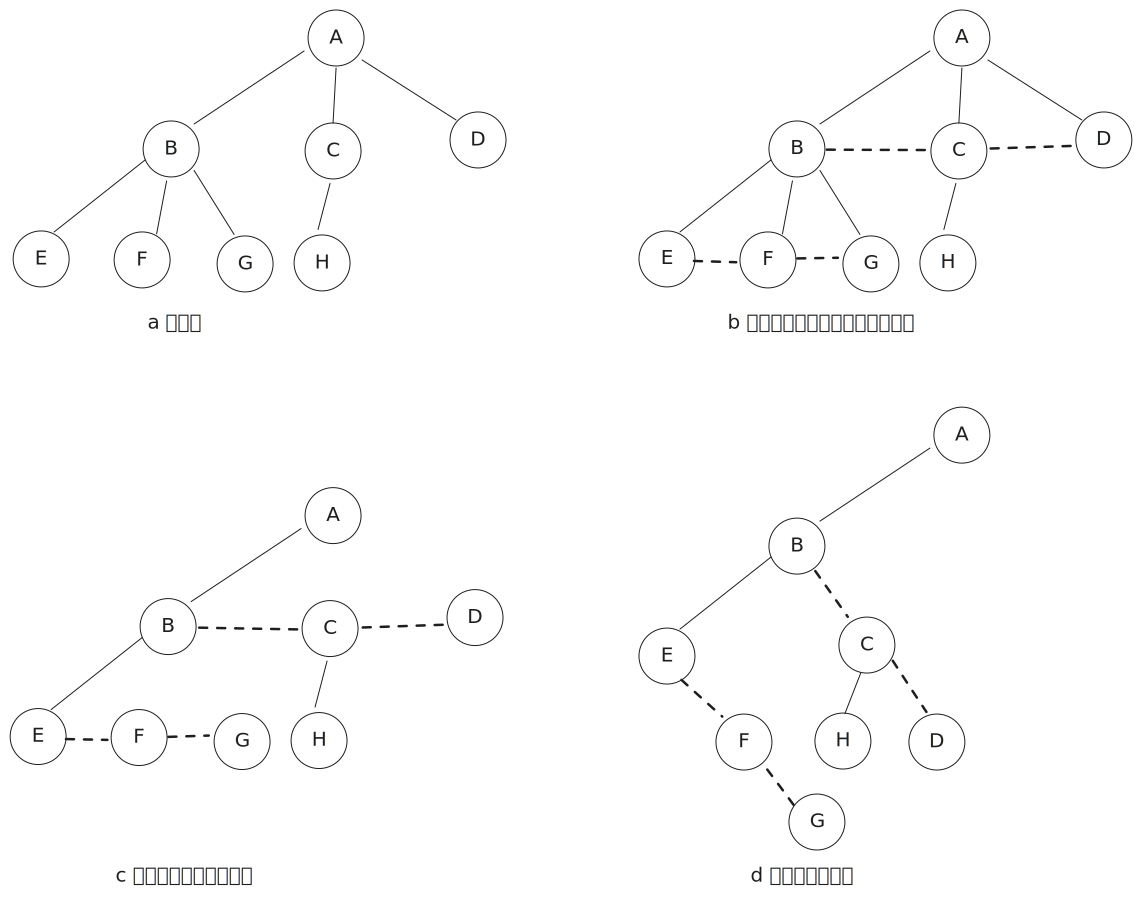
\includegraphics[width=1\textwidth]{./figure/pdf/cropped/tree2Btree.pdf}
  \caption{树转换成二叉树}
  \label{fig:tree2BiTree}
\end{figure}


若一棵二叉树是由一棵树转换而来的,则该二叉树还原为树的过程如下:

\begin{enumerate}
  \item 若某结点是其双亲的左孩子,则把该结点的右孩子、右孩子的右孩子等都与该结点的双亲结点用连线连起来;
  \item 删除原二叉树中所有双亲结点与右孩子结点之间的连线;
  \item 整理由前面两步得到的树,即以根结点为轴心,逆时针转动 $45^\circ$,使之结构层次分明。
\end{enumerate}

实际上,二叉树的还原就是将二叉树中的左分支保持不变,将二叉树中的右分支还原成兄弟关系。

如图\ref{fig:BiTree2Tree}所示,将二叉树还原成树的过程。

\begin{figure}[h!]
  \centering
  \includegraphics[width=1\textwidth]{./figure/pdf/cropped/Btree2Tree.pdf}
  \caption{二叉树还原成树}
  \label{fig:BiTree2Tree}
\end{figure}


\subsection{二叉树和森林的转换}

将一棵森林转换成二叉树的过程如下:
\begin{enumerate}
  \item 将森林中的每棵树转换成相应的二叉树;
  \item 第一棵二叉树不动,从第二棵二叉树开始,依次把后一棵二叉树的根结点作为前一棵二叉树根结点的右孩子结点。
  当所有二叉树连在一起后,此时得到的二叉树就是由森林转换得到的二叉树。
\end{enumerate}

实际上,当森林由两棵或两棵以上的树 $\{T_1, T_2, \dots, T_n\}$ 构成时,所有这些树的根结点构成兄弟关系。所以森林转换成一棵二叉树 $BT$ 后,
将第一棵树 $T_1$ 的根结点作为 $BT$ 的根结点,$T_2$ 的根结点作为 $T_1$ 的右孩子结点,$T_3$ 的根结点作为 $T_2$ 的右孩子结点,依此类推。

如图\ref{fig:forest2BiTree}所示,将森林转换成二叉树的过程。

\begin{figure}[h!]
  \centering
  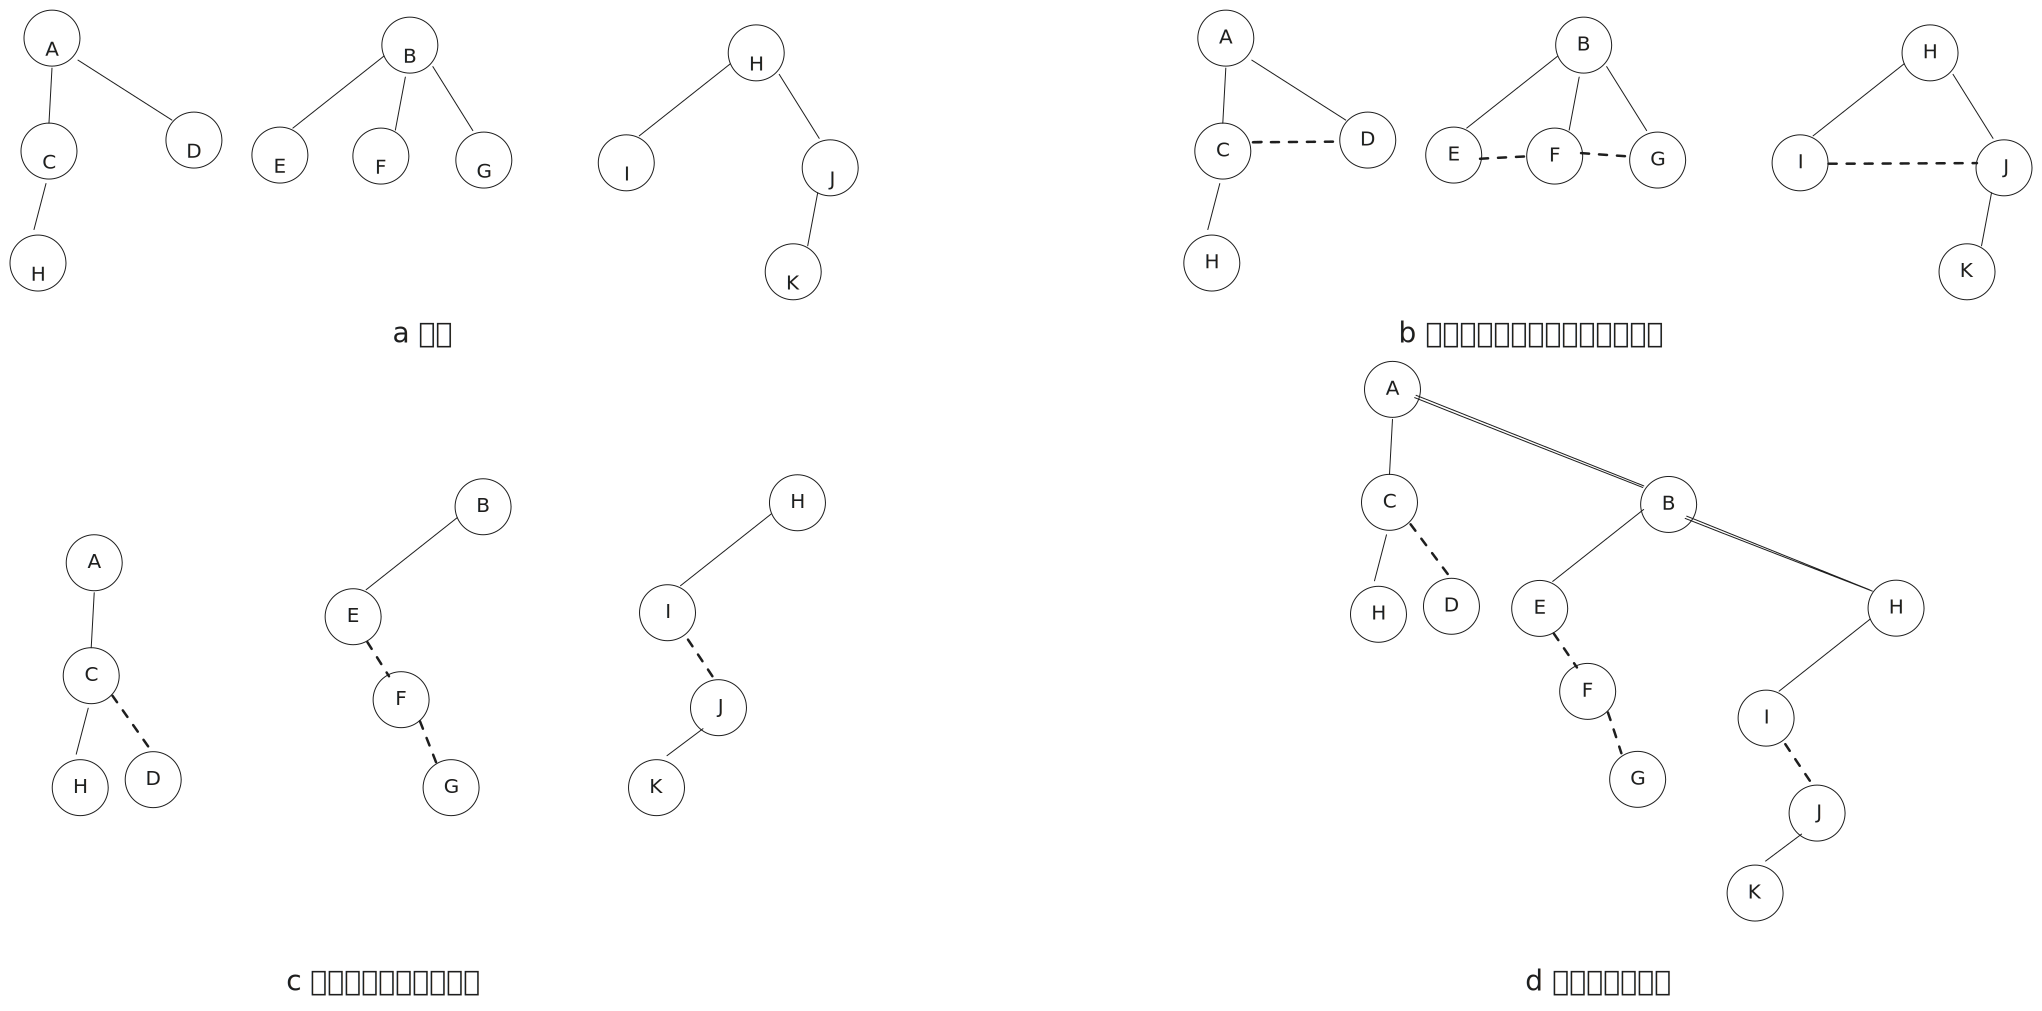
\includegraphics[width=1\textwidth]{./figure/pdf/cropped/forest2Btree.pdf}
  \caption{森林转换成二叉树}
  \label{fig:forest2BiTree}
\end{figure}

将二叉树还原为森林的过程如下:

\begin{enumerate}
  \item 抹掉二叉树根结点右链上的所有结点之间的“双亲—右孩子”关系,将其分成若干个以右链上的结点为根结点的二叉树,
  设这些二叉树为 $BT_1, BT_2, \dots, BT_n$;
  \item 分别将 $BT_1, BT_2, \dots, BT_n$ 二叉树各自还原成一棵树。
\end{enumerate}

如图\ref{fig:BiTree2Forest}所示,将二叉树还原成森林的过程。

\begin{figure}[h!]
  \centering
  \includegraphics[width=1\textwidth]{./figure/pdf/cropped/Btree2Forest.pdf}
  \caption{二叉树还原成森林}
  \label{fig:BiTree2Forest}

\end{figure}
\subsection{哈夫曼树和哈夫曼编码}

\subsection{并查集}

\chapter{图}

\section{图的基本概念}

\subsection{图的定义}

\subsection{图的分类}

\subsection{图的基本术语}

\section{图的存储结构}

\subsection{邻接矩阵}

\subsection{邻接表}

\subsection{十字链表}

\subsection{邻接多重表}

\section{图的遍历}

\subsection{深度优先搜索}

\subsection{广度优先搜索}

\section{最小生成树}

\subsection{Prim算法}

\subsection{Kruskal算法}

\section{最短路径}

\subsection{Dijkstra算法}

\subsection{Floyd算法}

\section{拓扑排序}

\section{关键路径}

\chapter{查找}

\section{查找的基本概念}

\subsection{查找的定义}

\subsection{查找的基本术语}

\section{顺序查找}

\section{折半查找}

\section{分块查找}

\section{哈希查找}

\section{红黑树}

\section{B树}

\section{B+树}

\chapter{排序}

\section{排序的基本概念}

\subsection{排序的定义}

\subsection{排序的基本术语}

\section{插入排序}

\subsection{直接插入排序}

\subsection{希尔排序}

\section{交换排序}

\subsection{冒泡排序}

\subsection{快速排序}

\section{选择排序}

\subsection{直接选择排序}

\subsection{堆排序}

\section{归并排序}

\section{基数排序}

\section{排序算法的比较}

\section{外部排序}

\end{document}
